% Options for packages loaded elsewhere
% Options for packages loaded elsewhere
\PassOptionsToPackage{unicode}{hyperref}
\PassOptionsToPackage{hyphens}{url}
\PassOptionsToPackage{dvipsnames,svgnames,x11names}{xcolor}
%
\documentclass[
  a4paper,
  DIV=11,
  numbers=noendperiod,
  oneside]{scrreprt}
\usepackage{xcolor}
\usepackage{amsmath,amssymb}
\setcounter{secnumdepth}{5}
\usepackage{iftex}
\ifPDFTeX
  \usepackage[T1]{fontenc}
  \usepackage[utf8]{inputenc}
  \usepackage{textcomp} % provide euro and other symbols
\else % if luatex or xetex
  \usepackage{unicode-math} % this also loads fontspec
  \defaultfontfeatures{Scale=MatchLowercase}
  \defaultfontfeatures[\rmfamily]{Ligatures=TeX,Scale=1}
\fi
\usepackage{lmodern}
\ifPDFTeX\else
  % xetex/luatex font selection
\fi
% Use upquote if available, for straight quotes in verbatim environments
\IfFileExists{upquote.sty}{\usepackage{upquote}}{}
\IfFileExists{microtype.sty}{% use microtype if available
  \usepackage[]{microtype}
  \UseMicrotypeSet[protrusion]{basicmath} % disable protrusion for tt fonts
}{}
\makeatletter
\@ifundefined{KOMAClassName}{% if non-KOMA class
  \IfFileExists{parskip.sty}{%
    \usepackage{parskip}
  }{% else
    \setlength{\parindent}{0pt}
    \setlength{\parskip}{6pt plus 2pt minus 1pt}}
}{% if KOMA class
  \KOMAoptions{parskip=half}}
\makeatother
% Make \paragraph and \subparagraph free-standing
\makeatletter
\ifx\paragraph\undefined\else
  \let\oldparagraph\paragraph
  \renewcommand{\paragraph}{
    \@ifstar
      \xxxParagraphStar
      \xxxParagraphNoStar
  }
  \newcommand{\xxxParagraphStar}[1]{\oldparagraph*{#1}\mbox{}}
  \newcommand{\xxxParagraphNoStar}[1]{\oldparagraph{#1}\mbox{}}
\fi
\ifx\subparagraph\undefined\else
  \let\oldsubparagraph\subparagraph
  \renewcommand{\subparagraph}{
    \@ifstar
      \xxxSubParagraphStar
      \xxxSubParagraphNoStar
  }
  \newcommand{\xxxSubParagraphStar}[1]{\oldsubparagraph*{#1}\mbox{}}
  \newcommand{\xxxSubParagraphNoStar}[1]{\oldsubparagraph{#1}\mbox{}}
\fi
\makeatother


\usepackage{longtable,booktabs,array}
\usepackage{calc} % for calculating minipage widths
% Correct order of tables after \paragraph or \subparagraph
\usepackage{etoolbox}
\makeatletter
\patchcmd\longtable{\par}{\if@noskipsec\mbox{}\fi\par}{}{}
\makeatother
% Allow footnotes in longtable head/foot
\IfFileExists{footnotehyper.sty}{\usepackage{footnotehyper}}{\usepackage{footnote}}
\makesavenoteenv{longtable}
\usepackage{graphicx}
\makeatletter
\newsavebox\pandoc@box
\newcommand*\pandocbounded[1]{% scales image to fit in text height/width
  \sbox\pandoc@box{#1}%
  \Gscale@div\@tempa{\textheight}{\dimexpr\ht\pandoc@box+\dp\pandoc@box\relax}%
  \Gscale@div\@tempb{\linewidth}{\wd\pandoc@box}%
  \ifdim\@tempb\p@<\@tempa\p@\let\@tempa\@tempb\fi% select the smaller of both
  \ifdim\@tempa\p@<\p@\scalebox{\@tempa}{\usebox\pandoc@box}%
  \else\usebox{\pandoc@box}%
  \fi%
}
% Set default figure placement to htbp
\def\fps@figure{htbp}
\makeatother





\setlength{\emergencystretch}{3em} % prevent overfull lines

\providecommand{\tightlist}{%
  \setlength{\itemsep}{0pt}\setlength{\parskip}{0pt}}



 


\usepackage{unicode-math}%
\setmathfont{XITS Math}%
\usepackage{fontspec}%
\setmainfont[Ligatures ={Common, TeX}, Scale=1, RawFeature={+cpsp}]{XITS} 
%Numbers={Lining,Proportional},Ligatures ={Common, TeX},RawFeature={+tnum,+cpsp,+frac},
\setsansfont[RawFeature={+cpsp},Scale=MatchLowercase]{Helvetica Neue}%
\setmonofont[Scale=0.78]{Andale Mono}%

\usepackage[a4paper,%
margin=2.5cm,%
bottom=3cm,%
top=3cm]{geometry}%
\usepackage{afterpage}% for "\afterpage"
\usepackage{xcolor}%
\definecolor{dundeeblue}{HTML}{4365E2}%
\usepackage{pagecolor}% With option pagecolor={somecolor or none}
%% For nice tables
\usepackage{booktabs}%
\usepackage{longtable}%
\usepackage{array}%
\usepackage{multirow}%
\usepackage{wrapfig}%
\usepackage{float}%
\usepackage{colortbl}%
\usepackage{pdflscape}%
\usepackage{tabu}%
%\usepackage{threeparttable}%
%\usepackage{threeparttablex}%
%\usepackage[normalem]{ulem}%
\usepackage{makecell}%
%% Wrap long output lines
\usepackage{listings}%
\lstset{breaklines=true}%
\usepackage{enumitem}%
\setlist[description]{style=nextline}%
%% For nice info boxes
\usepackage{fontawesome5}%
\usepackage{awesomebox}%
\usepackage{siunitx}%
\newcolumntype{d}{S[table-format=3.2]}%
\renewcommand{\bibname}{References}%
%\usepackage[colorlinks]{hyperref}%

\usepackage{titling}%
%\setlength{\droptitle}{8cm}
\pretitle{\newpagecolor{dundeeblue}\afterpage{\restorepagecolor} \vfill \begin{flushleft}
\fontsize{68pt}{62pt} \color{white}\sffamily\bfseries\selectfont }
\posttitle{\end{flushleft}}

\preauthor{\vspace{2.5cm} \begin{flushleft} \fontsize{18pt}{14pt} \color{white}\sffamily\selectfont}
\postauthor{$\quad\bullet\quad$ghornig@dundee.ac.uk\end{flushleft}}

\predate{\begin{flushleft} \fontsize{18pt}{14pt} \color{white}\sffamily\selectfont}
\postdate{\\ \vspace{1cm}
\includegraphics[width=10cm]{assets/images/rev_logo.pdf}\end{flushleft}}

%%% BEGIN SHORTCUTS
%\DeclareMathOperator{\E}{\mathbf{E}}%
%\DeclareMathOperator{\Var}{Var}%
%\DeclareMathOperator{\Cov}{Cov}%
%\DeclareMathOperator{\corr}{corr}%
%\DeclareMathOperator{\sd}{sd}%
%\newcommand{\se}{\mathsf{se}}%
%%% END SHORTCUTS

%% Change chapter to Topic
\makeatletter
\renewcommand{\@chapapp}{Topic}
\makeatother

\usepackage{tocbibind}

\DeclareOldFontCommand{\rm}{\normalfont\rmfamily}{\mathrm}
\DeclareOldFontCommand{\sf}{\normalfont\sffamily}{\mathsf}
\DeclareOldFontCommand{\tt}{\normalfont\ttfamily}{\mathtt}
\DeclareOldFontCommand{\bf}{\normalfont\bfseries}{\mathbf}
\DeclareOldFontCommand{\it}{\normalfont\itshape}{\mathit}
\DeclareOldFontCommand{\sl}{\normalfont\slshape}{\@nomath\sl}
\DeclareOldFontCommand{\sc}{\normalfont\scshape}{\@nomath\sc}
\DeclareRobustCommand*\cal{\@fontswitch\relax\mathcal}
\DeclareRobustCommand*\mit{\@fontswitch\relax\mathnormal}
\KOMAoption{captions}{tableheading}
\makeatletter
\@ifpackageloaded{tcolorbox}{}{\usepackage[skins,breakable]{tcolorbox}}
\@ifpackageloaded{fontawesome5}{}{\usepackage{fontawesome5}}
\definecolor{quarto-callout-color}{HTML}{909090}
\definecolor{quarto-callout-note-color}{HTML}{0758E5}
\definecolor{quarto-callout-important-color}{HTML}{CC1914}
\definecolor{quarto-callout-warning-color}{HTML}{EB9113}
\definecolor{quarto-callout-tip-color}{HTML}{00A047}
\definecolor{quarto-callout-caution-color}{HTML}{FC5300}
\definecolor{quarto-callout-color-frame}{HTML}{acacac}
\definecolor{quarto-callout-note-color-frame}{HTML}{4582ec}
\definecolor{quarto-callout-important-color-frame}{HTML}{d9534f}
\definecolor{quarto-callout-warning-color-frame}{HTML}{f0ad4e}
\definecolor{quarto-callout-tip-color-frame}{HTML}{02b875}
\definecolor{quarto-callout-caution-color-frame}{HTML}{fd7e14}
\makeatother
\makeatletter
\@ifpackageloaded{bookmark}{}{\usepackage{bookmark}}
\makeatother
\makeatletter
\@ifpackageloaded{caption}{}{\usepackage{caption}}
\AtBeginDocument{%
\ifdefined\contentsname
  \renewcommand*\contentsname{Table of contents}
\else
  \newcommand\contentsname{Table of contents}
\fi
\ifdefined\listfigurename
  \renewcommand*\listfigurename{List of Figures}
\else
  \newcommand\listfigurename{List of Figures}
\fi
\ifdefined\listtablename
  \renewcommand*\listtablename{List of Tables}
\else
  \newcommand\listtablename{List of Tables}
\fi
\ifdefined\figurename
  \renewcommand*\figurename{Figure}
\else
  \newcommand\figurename{Figure}
\fi
\ifdefined\tablename
  \renewcommand*\tablename{Table}
\else
  \newcommand\tablename{Table}
\fi
}
\@ifpackageloaded{float}{}{\usepackage{float}}
\floatstyle{ruled}
\@ifundefined{c@chapter}{\newfloat{codelisting}{h}{lop}}{\newfloat{codelisting}{h}{lop}[chapter]}
\floatname{codelisting}{Listing}
\newcommand*\listoflistings{\listof{codelisting}{List of Listings}}
\usepackage{amsthm}
\theoremstyle{definition}
\newtheorem{example}{Example}[chapter]
\theoremstyle{remark}
\AtBeginDocument{\renewcommand*{\proofname}{Proof}}
\newtheorem*{remark}{Remark}
\newtheorem*{solution}{Solution}
\newtheorem{refremark}{Remark}[chapter]
\newtheorem{refsolution}{Solution}[chapter]
\makeatother
\makeatletter
\makeatother
\makeatletter
\@ifpackageloaded{caption}{}{\usepackage{caption}}
\@ifpackageloaded{subcaption}{}{\usepackage{subcaption}}
\makeatother
\makeatletter
\@ifpackageloaded{tcolorbox}{}{\usepackage[many]{tcolorbox}}
\makeatother
%%%% ---foldboxy preamble ----- %%%%%

\definecolor{fbx-default-color1}{HTML}{c7c7d0}
\definecolor{fbx-default-color2}{HTML}{a3a3aa}

\definecolor{fbox-color1}{HTML}{c7c7d0}
\definecolor{fbox-color2}{HTML}{a3a3aa}

% arguments: #1 typelabelnummer: #2 titel: #3
\newenvironment{fbx}[3]{\begin{tcolorbox}[enhanced, breakable,%
attach boxed title to top*={xshift=1.4pt},
boxed title style={boxrule=0.0mm, fuzzy shadow={1pt}{-1pt}{0mm}{0.1mm}{gray}, arc=.3em, rounded corners=east, sharp corners=west}, colframe=#1-color2, colbacktitle=#1-color1, colback = white, coltitle=black,  titlerule=0mm, toprule=0pt, bottomrule=.7pt, leftrule=.3em, rightrule=0pt, outer arc=.3em,  arc=0pt,	 sharp corners = east, left=.5em, bottomtitle=1mm, toptitle=1mm,title=\textbf{#2}\hspace{0.5em}{#3}]}
{\end{tcolorbox}}

% boxed environment with right border
\newenvironment{fbxSimple}[3]{\begin{tcolorbox}[enhanced, breakable,%
attach boxed title to top*={xshift=1.4pt},
boxed title style={boxrule=0.0mm, fuzzy shadow={1pt}{-1pt}{0mm}{0.1mm}{gray}, arc=.3em, rounded corners=east, sharp corners=west}, colframe=#1-color2, colbacktitle=#1-color1, colback = white, coltitle=black,  titlerule=0mm, toprule=0pt, bottomrule=.7pt, leftrule=.3em, rightrule=.7pt, outer arc=.3em,  	left=.5em, right=.5em, bottomtitle=1mm, toptitle=1mm,title=\textbf{#2}\hspace{0.5em}{#3}]}
{\end{tcolorbox}}

%%%% --- end foldboxy preamble ----- %%%%%
%%==== colors from yaml ===%
\definecolor{Lemma-color1}{HTML}{948bde}
\definecolor{Lemma-color2}{HTML}{584eab}
\definecolor{Theorem-color1}{HTML}{948bde}
\definecolor{Theorem-color2}{HTML}{584eab}
\definecolor{Feature-color1}{HTML}{c0c0c0}
\definecolor{Feature-color2}{HTML}{808080}
\definecolor{DONE-color1}{HTML}{cce7b1}
\definecolor{DONE-color2}{HTML}{86b754}
\definecolor{Definition-color1}{HTML}{d999d3}
\definecolor{Definition-color2}{HTML}{a01793}
\definecolor{Proof-color1}{HTML}{c0c0c0}
\definecolor{Proof-color2}{HTML}{808080}
\definecolor{Solution-color1}{HTML}{c0c0c0}
\definecolor{Solution-color2}{HTML}{808080}
\definecolor{Corollary-color1}{HTML}{948bde}
\definecolor{Corollary-color2}{HTML}{584eab}
\definecolor{Conjecture-color1}{HTML}{948bde}
\definecolor{Conjecture-color2}{HTML}{584eab}
\definecolor{TODO-color1}{HTML}{e7b1b4}
\definecolor{TODO-color2}{HTML}{8c3236}
%=============%
\newcounter{quartocalloutnteno}
\newcommand{\quartocalloutnte}[1]{\refstepcounter{quartocalloutnteno}\label{#1}}
\usepackage{bookmark}
\IfFileExists{xurl.sty}{\usepackage{xurl}}{} % add URL line breaks if available
\urlstyle{same}
\hypersetup{
  pdftitle={Core Mathematics III},
  pdfauthor={Prof Gunnar Hornig},
  colorlinks=true,
  linkcolor={blue},
  filecolor={Maroon},
  citecolor={Blue},
  urlcolor={Blue},
  pdfcreator={LaTeX via pandoc}}


\title{Core Mathematics III}
\author{Prof Gunnar Hornig}
\date{2025-09-22}
\begin{document}
\maketitle

\renewcommand*\contentsname{Table of contents}
{
\hypersetup{linkcolor=}
\setcounter{tocdepth}{2}
\tableofcontents
}

\bookmarksetup{startatroot}

\chapter*{Introduction}\label{introduction}
\addcontentsline{toc}{chapter}{Introduction}

\markboth{Introduction}{Introduction}

Welcome to MA21001 at the University of Dundee.

These notes are available at
\href{https://dundeemath.github.io/MA21001/}{dundeemath.github.io/MA21001/}
as HTML and also as a PDF.

\section*{Licence}\label{licence}
\addcontentsline{toc}{section}{Licence}

\markright{Licence}

\pandocbounded{
\includegraphics[keepaspectratio]{index_files/mediabag/88x31.png}}

This work is licensed under a
\href{http://creativecommons.org/licenses/by-nc/4.0/}{Creative Commons
Attribution-NonCommercial 4.0 International License}.

\part{Algebra}

\chapter{Before we start \ldots{}}\label{before-we-start}

\section{Linear Algebra}\label{linear-algebra}

\emph{Algebra: The department of mathematics which investigates the
relations and properties of numbers by means of general symbols; and, in
a more abstract sense, a calculus of symbols combining according to
certain defined laws (Oxford English Dictionary)}

Linear algebra is the branch of mathematics concerned with the study of
vectors, vector spaces (also called linear spaces), linear
transformations, and systems of linear equations. Vector spaces are a
central theme in modern mathematics; thus, linear algebra is widely used
in both abstract algebra and functional analysis. Linear algebra also
has a concrete representation in analytic geometry and is generalised in
operator theory. It has extensive applications in the natural sciences
and the social sciences since a linear model can often approximate
nonlinear models.

The name Algebra (from Arabic: al-jabr) is derived from the treatise
written by the Persian mathematician Muhammad ibn Musa al-Kwarizmi
titled \emph{Al-Kitab al-Jabr wa-l-Muqabala}, meaning ``The Compendious
Book on Calculation by Completion and Balancing", which provided
symbolic operations for the systematic solution of linear and quadratic
equations \footnote{From Wikipedia, the free encyclopaedia}.

\section{The Language of Mathematics}\label{the-language-of-mathematics}

To formulate mathematics, we first have to define the notions we are
using before we make any statement. This allows us to prove general
statements, which is the essence of mathematics. Mathematical notions
are defined in Axioms and Definitions, while statements are called
Theorems or Corollaries:

\subsection{Axioms}\label{axioms}

a fundamental definition or statement which can't be derived from any
simpler statement. Axioms are the starting points of a mathematical
theory. Often, axioms are so "self-evident" that they are not explicitly
mentioned.

Example: "Peano Axioms" for the natural numbers.

\begin{enumerate}
\def\labelenumi{\arabic{enumi}.}
\item
  0 is a natural number.
\item
  For every natural number n, the successor, S(n), is a natural number.
\item
  For every natural number n, \(S(n) \neq 0\). That is, there is no
  natural number whose successor is 0.
\item
  For all natural numbers m and n, if S(m) = S(n), then m = n.~That is,
  S is an injection.
\end{enumerate}

The original Peano axioms (published in 1889 by the Italian
mathematician Giuseppe Peano) also included a set of axioms for the
notion of equality and one further ``axiom of induction".

\begin{enumerate}
\def\labelenumi{\arabic{enumi}.}
\item
  For every natural number x, x = x. That is, equality is reflexive.
\item
  For all natural numbers x and y, if x = y, then y = x. That is,
  equality is symmetric.
\item
  For all natural numbers x, y and z, if x = y and y = z, then x = z.
  That is, equality is transitive.
\item
  For all a and b, if a is a natural number and a = b, then b is also a
  natural number. That is, the natural numbers are closed under
  equality.
\item
  If K is a set such that 0 is in K, and for every natural number n, if
  n is in K, then S(n) is in K, then K contains every natural number.
  (axiom of induction)
\end{enumerate}

\subsection{Definition}\label{definition}

A new mathematical notion is given (defined) in terms of existing
notions.

Example: \emph{A rational number is any number that can be expressed as
the quotient a/b of two integers, with the denominator b not equal to
zero.} Note that this definition requires to know what integers are and
the notion of division (quotient).

\subsection{Theorem}\label{theorem}

A statement which relates specific (perviously defined) mathematical
properties. It usually requires proof using definitions and mathematical
logic to show the statement is true.

\subsection{Corollary, Lemma}\label{corollary-lemma}

An immediate consequence of a theorem (Corollary) or a minor theorem
(Lemma). Sometimes, it comes with a proof; sometimes, it is omitted
because it is considered trivial.

\emph{Example 1.1}. As an example let's define something new :

\textbf{Definition 1.1}. An umpf is a natural number, which is a
multiple of 3. A gumpf is a natural number which is a multiple of 6.
(These are made-up notions, just for demonstration)

\textbf{Lemma 1.1}. \emph{Every gumpf is an umpf.}

\begin{proof}
If x is a gumpf, then \(x= 6 n\), where n is a natural number. Hence
\(x=3 \cdot 2 \cdot n = 3 \cdot (2\cdot n)\). Therefore, x is an umpf.~◻
\end{proof}

The end of a proof is often indicated by a square or the abbreviation
q.e.d. (Latin: quod erat demonstrandum) ``that which was to be shown''.

\section{Mathematical notation}\label{mathematical-notation}

\subsection*{Symbols}\label{symbols}
\addcontentsline{toc}{subsection}{Symbols}

\[\begin{aligned}
\mathbb{N}: \quad &  \text{natural numbers, e.g.} 1,2,...\\
\mathbb{Z}: \quad &  \text{integers: } .., -2,-1,0,1,2,...\\
\mathbb{Q}: \quad &  \text{rational numbers: } 0, 1/3, -5/11,...\\
\mathbb{R}: \quad &  \text{real numbers: } 0, \pi, \sqrt{2}, 2/3, -2, ...\\
\mathbb{C}: \quad &  \text{complex numbers: } 0, i, \pi +i, \sqrt{2}-4i , -2/3,  ...\\
\Rightarrow \quad &  \text{logical implication, } A \Rightarrow B: \ \text{if A then B} \\
\Leftrightarrow \quad &  \text{logical equivalence, }  A \Leftrightarrow B: \ \text{if A then B and if B then A} \\
\vee \quad & \text{logical {\it or}, }  A \vee B: \ \text{either A or B or both} \\
\land \quad & \text{logical {\it and},  }  A \land B: \ \text{A and B} \\
\in \quad &  \text{\it is an element of,} \ x \in \mathbb{R} : \ \text{x is an element of } \mathbb{R} \\
\forall \quad &  \text{{\it for all}, e.g.: }  x^{n} \in \mathbb{R} \  \forall \ n: \  \  \ x^{n}\text{ is real for all n} \\
\exists \quad &  \text{{\it there  exist(s)}, e.g.: }  \forall x\in \mathbb{Q} \ \exists \ p,q \in \mathbb{Z} \text{ with } x=p/q
\end{aligned}\]

See also the list of Greek letters in the Appendix
Section~\ref{sec-greekletters}.

\section{Mathematical proofs}\label{mathematical-proofs}

A sequence of logical arguments which shows that a statement is true in
all cases, without a single exception. Types of proofs are:

\begin{itemize}
\item
  direct proof.\\
  Example: The product of two even numbers is even. Proof: Let a,b two
  even numbers, that is \(a=2 n\) and \(b= 2 m\), where
  \(m,n \in \mathbb{Z}\). \(\Rightarrow\) \(ab= 2n 2m = 2 (2nm)\) is an
  even number.
\item
  proof by induction.\\
  This type of proof is often used to prove an infinite series of
  statements \(A_n\), \(n=1,2,3 \ldots\). If we can prove that a)
  \(A_1\) is true and b) if \(A_n\) is true then \(A_{n+1}\) is true,
  then \(A_n\) is true for all \(n \in \mathbb{N}\).

  Example: \(\sum_{n=1}^N n = \frac{1}{2} N (N+1)\)

  \begin{proof}
  \leavevmode

  \begin{enumerate}
  \def\labelenumi{\alph{enumi})}
  \tightlist
  \item
    The statement is true for \(n=1\): \(1=\frac{2}{2}\). b) If the
    formula is true for N=k then it is also true for N=k+1:
    \(\sum_{n=1}^N n = \frac{1}{2} N (N+1)\) \(\Rightarrow\)
    \(\sum_{n=1}^{N+1} n = \frac{1}{2} N (N+1) + (N+1) = (N+2)(N+1)/2\).~◻
  \end{enumerate}

  \end{proof}
\item
  proof by contradiction. The type of proof uses \(\neg (\neg A) = A\);
  that is, it is shown that the opposite statement \(\neg A\) is false
  (or \(\neg (\neg A)\) is true) and hence A is true.\\
  A famous example is the proof that \(\sqrt{2}\) is not a rational
  number: A: ``\(\sqrt{2}\) is not a rational number''. Let us assume
  \(\neg A\) is true, that is, \(\sqrt{2}\) is a rational number. Then
  \(\sqrt{2} = p/q\) with \(p,q \in \mathbb{Z}\) with no common
  divisior. \(\Rightarrow  2q^2=p^2\) \(\Rightarrow\) \(p^2\) is even
  and therefore \(p\) is even. Then \(p=2n \Rightarrow p^2=2^2 n^2\) and
  hence \(q^2= p^2/2=2 n^2\) is even. Therefore, \(q\) must be even in
  contradiction to the assumption that \(p,q\) had no common divisor.
\end{itemize}

\chapter{Vector spaces}\label{vector-spaces}

\section{Motivation}\label{motivation}

You have used vectors in previous modules to do elementary geometry.
These vectors were introduced as lines connecting two points with a
direction: \[{\vec a} = \overrightarrow{PQ},\] where \(P\) is the
starting point of the vector and \(Q\) is the endpoint. The space of all
these vectors is called the Euclidean space. It is usually introduced as
a two- or three-dimensional space, but it is possible to generalise this
to more dimensions. The Euclidean space was introduced as a simple model
for the physical space around us. One can furthermore introduce
orthogonal coordinates for the points in this space, e.g.
\[P =  (P_x,P_y,P_z) = (3,2,1).\] and this then allows us to define the
components of a vector:
\[{\vec a} = \overrightarrow{PQ} =  \begin{pmatrix}    Q_x- P_x \\ Q_y- P_y \\ Q_z -P_z  \end{pmatrix} \]
The identification between points and vectors in an Euclidean space
becomes particularly simple if we can choose \(P\) to be the origin of
the coordinate system, \(P=(0,0,0)\),
\[{\vec a} = \overrightarrow{OQ} =   \begin{pmatrix}    Q_x \\ Q_y \\ Q_z  \end{pmatrix} .\]
Note that while the coordinates of points are usually denoted by a row
of numbers (tuplet), the components of vectors are written as a column.
An alternative way to write a vector is to write it as a sum of
multiples of unit vectors,
\[{\vec v} =   v_x {\bf e}_x + v_y {\bf e}_y + v_z {\bf e}_z  =  \begin{pmatrix}    v_x \\ v_y \\ v_z  \end{pmatrix}.\]
An addition as well as a scalar multiplication was defined for these
vectors. Later, the scalar product between two vectors and the
cross-product (vector product) were also defined.

The operations on vectors of this Euclidean space \(E\), the addition
and scalar multiplication, had certain properties, for instance

\begin{itemize}
\tightlist
\item
  \(\vec{u} + \vec{v}  \in  E\), closure condition for addition
\item
  \(\vec{u}+\vec{v}  =  \vec{v}+\vec{u}\), the addition is commutative
\item
  \(\lambda (\vec{u}+ \vec{v})  =  \lambda \vec{u} + \lambda \vec{v}\),
  distributive law
\item
  \(\ldots\)
\end{itemize}

In the following, we will generalise this space and define an abstract
notion of a vector space, which has a much wider range of applications.
To understand the crucial properties of such a definition, consider two
examples.

\begin{example}[]\protect\hypertarget{exm-}{}\label{exm-}

The captain of a sailing boat can calculate the velocity of his ship
(speed and direction over ground) as the sum of two velocities: the
velocity of his boat relative to the water (speed through water) and the
velocity of the water (drift due to tides or ocean currents). The sum of
the two velocities is found in the same way as above, as the addition of
two vectors; however, the coordinate system used is usually a polar one
(the angle as determined by a compass and speed in knots) rather than a
Cartesian one (x, y-components). The velocities obtained this way are
part of a \emph{velocity space}. The elements of this space, the
velocities, follow the same rules of addition and scalar multiplication
as the vectors in our Euclidean space. Remark: In this example, the
velocity space is a tangent space to a manifold (the surface of the
ocean), a concept explained in more detail in Differential Geometry.

\end{example}

\begin{example}[]\protect\hypertarget{exm-}{}\label{exm-}

The set of all polynomials with degree \(\leq n\) is denoted by
\(\mathcal{P}_{n}\). We can add polynomials in \(\mathcal{P}_{n}\) to
obtain a polynomial in \(\mathcal{P}_{n}\) again. Polynomials
\(p(x)= a_{0} + a_{1}x + ...+a_{n} x^{n}\) and
\(q(x)= b_{0} + b_{1}x + ...+b_{n} x^{n}\)\(\in \mathcal{P}_{n}\) add up
to
\[p(x)+q(x)  =  (a_{0}+ b_{0}) + (a_{1} + b_{1}) x + ...+(a_{n}+ b_{n}) x^{n}   \in \mathcal{P}_{n} .\]
Similarly, we can multiply polynomials by a scalar
\[\lambda p(x)  =   \lambda a_{0} +  \lambda a_{1}x + ...+ \lambda a_{n} x^{n}  \in \mathcal{P}_{n}\]
Note that we can identify a polynomial of degree \(\leq n\) with the
vector of coefficients
\[p(x) \sim  \scriptstyle \begin{pmatrix}    a_{0} \\ a_{1} \\ \vdots \\ a_{n}   \end{pmatrix} \textstyle.\]

\end{example}

The two examples above illustrate that numerous diverse examples exist
where we find a structure similar to the Euclidean space. The elements
in these spaces often don't look like ``vectors"; they can be
polynomials, velocities, matrices, etc.\textasciitilde, but addition and
scalar multiplication work in the same way, so they follow the same
rules as vectors. This is the motivation to define an abstract notion of
a vector space and define it based on how its elements behave under
addition and scalar multiplication, rather than what they represent.

\section{Definition of a Vector
Space}\label{definition-of-a-vector-space}

\phantomsection\label{vksoverr}
\begin{fbxSimple}{Definition}{Definition 2.1: }{Vector Space over R}
\phantomsection\label{vksoverr}
A vector space over \(\mathbb{R}\) is a set \(V\), the elements of which
are called vectors \(\vec{v} \in V\) along with two operations, an
addition \(\vec{v} + \vec{w}\) and a scalar multiplication
\(a \vec{v}\), \(a \in \mathbb{R}\), subject to the following axioms for
all \(\vec{u},\vec{v}, \vec{w}\in V\) and \(a,b\in \mathbb{R}\) :
\begin{equation}\phantomsection\label{eq-cond0}{\vec{u} + \vec{v} \in  V}\end{equation}
\begin{equation}\phantomsection\label{eq-cond1}{a \vec{u}  \in  V}\end{equation}
\begin{equation}\phantomsection\label{eq-cond2}{\vec{u}+\vec{v} = \vec{v}+\vec{u}}\end{equation}
\begin{equation}\phantomsection\label{eq-cond3}{(\vec{u}+\vec{v})+\vec{w}  = \vec{u}+(\vec{v}+\vec{w})}\end{equation}
\begin{equation}\phantomsection\label{eq-cond4}{\text{there exists a vector } {\vec 0}  \in V \text{such that } \vec{u}+\vec{0} = \vec{0}+\vec{u}=\vec{u}}\end{equation}
\begin{equation}\phantomsection\label{eq-cond5}{ \text{given } \vec{v} \text{ there exists a vector } -\vec{v}  \in V  \text{ such that }\vec{v}+ (-\vec{v})  = \vec{0}}\end{equation}
\begin{equation}\phantomsection\label{eq-cond6}{1 \vec{u}  = \vec{u}}\end{equation}
\begin{equation}\phantomsection\label{eq-cond7}{a (\vec{u}+ \vec{v})  = a\vec{u} +a \vec{v}}\end{equation}
\begin{equation}\phantomsection\label{eq-cond8}{(a+b) \vec{u} = a\vec{u} +b \vec{u}}\end{equation}
\begin{equation}\phantomsection\label{eq-cond9}{a (b \vec{u}) =(a b) \vec{u}}\end{equation}

\end{fbxSimple}

Axiom \ref{eq-cond0} and \ref{eq-cond1} ensure that both operations do
not lead to elements not in \(V\), \ref{eq-cond2} to \ref{eq-cond5}
ensure that the addition is commutative and associative and that there
is a neutral element \(\vec{0}\) and an inverse element with respect to
the addition. Axiom \ref{eq-cond6} states that the neutral element of
the multiplication in \(\mathbb{R}\) is also the neutral element for the
scalar multiplication, while the remaining conditions are distributive
laws.

\begin{tcolorbox}[enhanced jigsaw, colback=white, leftrule=.75mm, title=\textcolor{quarto-callout-note-color}{\faInfo}\hspace{0.5em}{Remark on Notation}, toprule=.15mm, toptitle=1mm, titlerule=0mm, bottomrule=.15mm, opacitybacktitle=0.6, bottomtitle=1mm, coltitle=black, arc=.35mm, opacityback=0, breakable, colframe=quarto-callout-note-color-frame, rightrule=.15mm, left=2mm, colbacktitle=quarto-callout-note-color!10!white]

Alternative notations for vectors encountered in the literature are bold
face symbols \({\bf v}\) or \(\bar v\) (not to be confused with complex
conjugation) or \(\underline v\). The zero vector \(\vec{0}\) is often
written just as \(0\). Note that there are two kinds of additions in
this definition, both denoted by the same symbol \(+\). The addition of
two real numbers (\(a+b\)) and the addition of two vectors
\(\vec{v}+\vec{w}\). Also, for the multiplication, we have
\(ab \in \mathbb{R}\) as well as \(a \vec{v} \in V\). No symbol is used
for multiplication, since the dot as well as the cross will be later
used to define two different types of multiplication between two
vectors.

If we want to avoid writing a vector as a column, as this always takes
up a lot of space, we can use the transpose (denoted by a superscript
T): \[ (1,2)^T = \begin{pmatrix}  1 \\ 2 \end{pmatrix} \].

\end{tcolorbox}

\begin{example}[]\protect\hypertarget{exm-vktspace1}{}\label{exm-vktspace1}

The set
\(\mathbb{R}^2 = \{(x_{1},x_{2})^T \vert x_{1} \in \mathbb{R}, x_{2} \in \mathbb{R}\}\)
is a vector space, the elements of which are written as columns
\(\vec{x}=\scriptstyle \begin{pmatrix}   x_{1}\\x_{2}  \end{pmatrix} \textstyle\),
if addition and multiplication are defined as
\[ \begin{pmatrix}   x_1 \\ x_2  \end{pmatrix} 
  +
   \begin{pmatrix}   y_1 \\ y_2  \end{pmatrix} 
  =
   \begin{pmatrix}   x_1+y_1 \\ x_2+y_2  \end{pmatrix} ;
  \qquad
  a 
   \begin{pmatrix}   x_1 \\ x_2  \end{pmatrix} 
  =
   \begin{pmatrix}   a x_1 \\  a x_2  \end{pmatrix}  \ .\] We have to
check that all the axioms \ref{eq-cond0} to \ref{eq-cond9} are
satisfied.

\begin{itemize}
\tightlist
\item
  axioms \ref{eq-cond0} and \ref{eq-cond1} are satisfied because the
  elements are again element in \(V\).
\item
  axioms \ref{eq-cond2} to \ref{eq-cond3} are satisfied because the
  addition of real numbers in each entry of the vector is associative
  and commutative,
\item
  \ref{eq-cond4} and \ref{eq-cond5} are correct if we use the following
  zero vector and negative element:
  \[\vec{0}=\scriptstyle \begin{pmatrix}   0\\0  \end{pmatrix} \textstyle \qquad   -\vec{x} = \scriptstyle \begin{pmatrix}   -x_{1}\\-x_{2}  \end{pmatrix} \textstyle \ .\]
\item
  axiom \ref{eq-cond6} is obvious from the definition of the scalar
  multiplication,
\item
  axiom \ref{eq-cond7}
  \[(r+s) \begin{pmatrix}   v_1 \\ v_2  \end{pmatrix} 
    =\begin{pmatrix}   (r+s)v_1 \\ (r+s)v_2  \end{pmatrix} 
    = \begin{pmatrix}   rv_1+sv_1 \\ rv_2+sv_2  \end{pmatrix} 
    =r \begin{pmatrix}   v_1 \\ v_2  \end{pmatrix} +s \begin{pmatrix}   v_1 \\ v_2  \end{pmatrix}; \]
\item
  axiom \ref{eq-cond8}
  \[r \left( \begin{pmatrix}   v_1 \\ v_2  \end{pmatrix} + \begin{pmatrix}   w_1 \\ w_2  \end{pmatrix} \right)
    =\begin{pmatrix}   r(v_1+w_1) \\ r(v_2+w_2)  \end{pmatrix} 
    =\begin{pmatrix}   rv_1+rw_1 \\ rv_2+rw_2  \end{pmatrix} 
    =r \begin{pmatrix}   v_1 \\ v_2  \end{pmatrix} +r \begin{pmatrix}   w_1 \\ w_2  \end{pmatrix}; \]
\item
  axiom \ref{eq-cond9}
  \[(rs) \begin{pmatrix}   v_1 \\ v_2  \end{pmatrix} 
    = \begin{pmatrix}   (rs)v_1 \\ (rs)v_2  \end{pmatrix} 
    =\begin{pmatrix}   r(sv_1) \\ r(sv_2)  \end{pmatrix} 
    =r \left(s \begin{pmatrix}   v_1 \\ v_2  \end{pmatrix} \right).\]
\end{itemize}

\end{example}

\begin{example}[]\protect\hypertarget{exm-vktspace2}{}\label{exm-vktspace2}

The set
\[V= \left\{ \left.  \begin{pmatrix}   v_{1}\\ v_{2}  \end{pmatrix}  \in \mathbb{R}^2 \right|  v_1^2+v_2^2 \le 1\right\}\]
with the addition and scalar multiplication as in the previous example
is \textbf{not} a vector space. The first two axioms (closure
conditions) are not satisfied. For example
\[{\bf u}=  \begin{pmatrix}   1/2\\ 1/2  \end{pmatrix}  \in V, \ \text{since} \    \left(\frac{1}{2}\right)^2+\left(\frac{1}{2}\right)^2 = \frac{1}{2} \le 1, \  \text{but} \quad  2{\bf u}= 2  \begin{pmatrix}   1/2\\ 1/2  \end{pmatrix}  = \begin{pmatrix}   1\\ 1  \end{pmatrix}   \notin V.\]

\end{example}

\begin{example}[]\protect\hypertarget{exm-vktspace3}{}\label{exm-vktspace3}

The set
\[V= \left\{ \left.  \begin{pmatrix}   v_{1}\\ v_{2}  \end{pmatrix}  \right| v_1 \in   \mathbb{R}, v_2 \in  \mathbb{R}\right\}\]
with the same scalar multiplication as before
\[a   \begin{pmatrix}   x_1 \\ x_2  \end{pmatrix}  =   \begin{pmatrix}   a x_1 \\  a x_2  \end{pmatrix}  \ ,\]
but the addition \[ \begin{pmatrix}   x_1 \\ x_2  \end{pmatrix} 
  +
  \begin{pmatrix}   y_1 \\ y_2  \end{pmatrix} \
  =\begin{pmatrix}   x_1+y_1+1 \\ x_2+y_2+1  \end{pmatrix}\] is
\textbf{not} a vector space. Axioms 8 and 9 are not satisfied.

\end{example}

\begin{example}[]\protect\hypertarget{exm-vktspace4}{}\label{exm-vktspace4}

What we have shown for a vector space consisting of two vectors with two
real components can be easily extended to n components. The vector space
\[I\!\!R^{n} = \left\{ \left. \scriptscriptstyle \begin{pmatrix}   v_{1}\\ v_{2} \\ \vdots \\ v_{n}  \end{pmatrix} \textstyle \right| v_{i} \in \mathbb{R}, i=1,2, .. ,n \right\}\]
together with the operation of addition
\[\scriptscriptstyle \begin{pmatrix}   v_{1}\\ v_{2} \\ \vdots \\ v_{n}  \end{pmatrix} \textstyle +  \scriptscriptstyle \begin{pmatrix}   w_{1}\\ w_{2} \\ \vdots \\ w_{n}  \end{pmatrix} \textstyle =  \scriptscriptstyle \begin{pmatrix}   v_{1}+w_{1}\\ v_{2} +w_{2}\\ \vdots \\ v_{n}+w_{n}  \end{pmatrix} \textstyle\]
and the scalar multiplication
\[ \alpha \scriptscriptstyle \begin{pmatrix}   v_{1}\\ v_{2} \\ \vdots \\ v_{n}  \end{pmatrix} \textstyle =  \scriptscriptstyle \begin{pmatrix}    \alpha v_{1}\\  \alpha v_{2} \\ \vdots \\  \alpha v_{n}  \end{pmatrix} \textstyle \quad \alpha \in \mathbb{R}\]
is called the vector space \(\mathbb{R}^{n}\).

Although we haven't defined yet what a basis is, we mention here for
future reference that the vectors,
\[\vec{e}_{1} =  \scriptscriptstyle \begin{pmatrix}   1\\ 0 \\ \vdots \\ 0   \end{pmatrix} \textstyle, \quad  \vec{e}_{2} =  \scriptscriptstyle \begin{pmatrix}   0\\ 1 \\ 0 \\ \vdots  \end{pmatrix} \textstyle, ...    ,\vec{e}_{n} =  \scriptscriptstyle \begin{pmatrix}   0\\ 0 \\ \vdots \\ 1   \end{pmatrix} \textstyle\]
form a basis of \(\mathbb{R}^{n}\), the so called the standard basis.
That is, every vector in \(\mathbb{R}^{n}\) can be expressed as a linear
combination of the basis vectors,
\[\vec{r} = r_{1} \vec{e}_{1} + r_{2} \vec{e}_{2} + ... + r_{n} \vec{e}_{n} ,\]
Or, in other words, the vector space is spanned by the basis vectors.

\end{example}

\begin{example}[]\protect\hypertarget{exm-vktspace5}{}\label{exm-vktspace5}

The set of all \(m\times n\) matrices where the entries are real numbers
forms a vector space. We denote this space by \(M^{(m \times n)}\).
Addition and scalar multiplication are the usual addition and scalar
multiplication of matrices. A basis of the space consists of the
matrices \({\rm E}^{(i,j)}\) which have a 1 at entry (i,j) and zeros
everywhere else. The space is of dimension \(m n\).

\end{example}

\begin{example}[]\protect\hypertarget{exm-vktspace6}{}\label{exm-vktspace6}

Let \(\mathcal{P}_{n}\) denote the set of all polynomials with degree
\(\leq n\). \(\mathcal{P}_{n}\) is a vector space if we declare an
addition and scalar multiplication of polynomials
\(p(x)= a_{0} + a_{1}x + ...+a_{n} x^{n}\) and
\(q(x)= b_{0} + b_{1}x + ...+b_{n} x^{n}\)\(\in \mathcal{P}_{n}\) by
\[\begin{aligned}
p(x)+q(x) &= (a_{0}+ b_{0}) + (a_{1} + b_{1}) x + ...+(a_{n}+ b_{n}) x^{n}   \in \mathcal{P}_{n} ,  \\
\lambda p(x) &=  \lambda a_{0} +  \lambda a_{1}x + ...+ \lambda a_{n} x^{n}  \in \mathcal{P}_{n} . 
\end{aligned}\] Note that we can identify a polynomial of degree
\(\leq n\) with the vector of coefficients
\[p(x) \sim  (a_{0}, a_{1},.., a_{n})^{T} .\] Hence, a basis for the
space consists of the \emph{monomials} \(x^{r}, r=0,1, ..,n\) and is
\(n+1\) dimensional.

\end{example}

\begin{example}[]\protect\hypertarget{exm-vktspace7}{}\label{exm-vktspace7}

The solutions of a homogeneous linear differential equation of order
\(n\), e.g.
\[\frac{\mathrm{d}^{2}y}{\mathrm{d}x^{2}}-3\frac{\mathrm{d}y}{\mathrm{d}x}
+2y=0.\qquad\] form a vector space. Addition and scalar multiplication
in this vector space are the usual addition and scalar multiplication of
functions. The space is spanned by \(n\) linearly independent solutions.
This is an example of a so-called \emph{function space}.

\end{example}

\begin{example}[]\protect\hypertarget{exm-vktspace8}{}\label{exm-vktspace8}

The set \(\mathcal{F}\) of all infinitely differentiable functions,
\(\mathbb{R} \rightarrow \mathbb{R}\), i.e., those~that have derivatives
of all orders. Note that (among others) the following functions belong
to \(\mathcal{F}\): \[e^{nx},\,\cos \left( 2\pi nx\right)
,\,\,x^{n}\quad \,(\text{for all }n=0,1,2,...).\] \(\mathcal{F}\) is an
example of an infinite-dimensional space because it contains an
unlimited number of linearly independent elements.

\end{example}

The definition of a vector space over \(\mathbb{R}\) can be extended to
a vector space over a more general set of numbers, a field K. To
understand what a `field' is, we need to take a short detour into number
systems.

\phantomsection\label{vksoverk}
\begin{fbxSimple}{Definition}{Definition 2.2: }{Vector Space over K}
\phantomsection\label{vksoverk}
A vector space over a field \(K\) is a set \(V\), the elements of which
are called vectors \(\vec{v} \in V\) along with two operations, an
addition \(\vec{v} + \vec{w}\) and a scalar multiplication
\(a \vec{v}\), \(a \in K\), subject to the same 10 axioms
Equation~\ref{eq-cond0} to Equation~\ref{eq-cond9} as before only that
now \(a,b\in K\).

\end{fbxSimple}

\begin{example}[]\protect\hypertarget{exm-vktspace9}{}\label{exm-vktspace9}

The set \hyperref[vksoverk]{2.2}
\(\mathbb{C}^{n} =\{ (c_{1},...,c_{n})^{T}| c_{1},..,c_{n}\in \mathbb{C}\}\)
is a vector space over \(\mathbb{C}\). Addition and scalar
multiplication are the usual addition and scalar multiplication of
complex numbers. A basis for this space is given by the n vectors
\(e_{1}=(1,0,...,0)\),..., \(e_{n}=(0,...,0,1)\). The space has \(n\)
dimensions. Note that we can identify \(\mathbb{C}\) with
\(\mathbb{R}^{2}\) due to \(z= a + b i\) with \(a,b \in \mathbb{R}\).
Hence \(\mathbb{C}^{n}  \sim \mathbb{R}^{2n}\) is also a vector space
over \(\mathbb{R}\), but in this case it is 2n-dimensional with two
basis vectors for the real and imaginary part of each complex dimension.

\end{example}

\section{Linear independence}\label{linear-independence}

In the same way as a coordinate system is introduced on a plane to
allocate a unique pair of coordinates to any point in the plane, we
would like to have a coordinate system for a vector space, which
uniquely assigns to any vector of this space a coordinate tuple (set).
To generate such a coordinate system, we need a set of `basis' vectors
which are, in a sense, independent. Consider the following example in
the x-y plane.

Given the two unit vectors in \(\mathbb{R}^2\),
\[\vec{e}_1 = \scriptstyle \begin{pmatrix}   1 \\ 0  \end{pmatrix} \textstyle, \ \vec{e}_2= \scriptstyle \begin{pmatrix}   0 \\ 1  \end{pmatrix} \textstyle\]
Any point in the plane, that is, any vector in \(\mathbb{R}^2\), can be
represented by a linear combination
\[\vec{v } = v_1  \vec{e}_1  + v_2  \vec{e}_2,  v_1,v_2 \in \mathbb{R}\]
where \((v_1,v_2)\) play the role of coordinates. These coordinates are
unique; that is, there are no two different vectors with the same
coordinate pair, nor are two different coordinate pairs assigned to the
same vector.

The same is true if we replace our basis vectors by (check!)
\[\vec{e}_1 = \scriptstyle \begin{pmatrix}   1 \\ 0  \end{pmatrix} \textstyle, \ \vec{e}_2= \scriptstyle \begin{pmatrix}   1 \\ 1  \end{pmatrix} \textstyle .\]

However, if we use a triplet of vectors:
\[\vec{e}_1 = \scriptstyle \begin{pmatrix}   1 \\ 0  \end{pmatrix} \textstyle, \ \vec{e}_2= \scriptstyle \begin{pmatrix}   0 \\ 1  \end{pmatrix} \textstyle,  \ \vec{e}_3= \scriptstyle \begin{pmatrix}   1 \\ 1  \end{pmatrix} \textstyle ,\]
\[\vec{v } = v_1  \vec{e}_1  + v_2  \vec{e}_2 + v_3  \vec{e}_3 ,  v_1,v_2,v_3 \in \mathbb{R}\]

Then there are vectors with non-unique coordinates:
\[\vec{v}   = 2  \vec{e}_1 + 3  \vec{e}_2 -1 \vec{e}_3  =   1  \vec{e}_1 + 2  \vec{e}_2 + 0 \vec{e}_3\]

More generally, if such a non-unique case occurs, one can write
\[\begin{aligned}
 {\bf v} & =   v_1  \vec{e}_1 +  v_2 \vec{e}_2 + v_3 \vec{e}_3 \\
  {\bf v} & =   v_1'  \vec{e}_1 + v_2'  \vec{e}_2 + v_3' \vec{e}_3 \\
  \Rightarrow \vec{0} & =   (v_1-v_1')  \vec{e}_1 + (v_2-v_2')  \vec{e}_2 + (v_3-v_3') \vec{e}_3, \\
   \Rightarrow   \vec{0} & =   a_1  \vec{e}_1 + a_2  \vec{e}_2 + a_3 \vec{e}_3, \quad (a_1,a_2,a_3) \neq (0,0,0) 
  \end{aligned}\] where at least one of the three brackets is non-zero
since we assumed that \((v_1,v_2,v_3) \neq (v_1',v_2',v_3')\). This is
called a non-trivial linear combination.

\phantomsection\label{linear-combination}
\begin{fbxSimple}{Definition}{Definition 2.3: }{Linear Combination}
\phantomsection\label{linear-combination}
An expression of the form \(a_{1}{\vec v}
_{1}+a_{2}{\vec v}_{2}+\cdots +a_{n}{\vec v}_{n}\) is known as a
\emph{linear combination of the \(n\) vectors \({\vec v}
_{1},{\vec v}_{2},\cdots ,{\vec v}_{n}\). The numbers
\(a_{1}, a_{2},..., a_{n}\) are known as the coefficients of the linear
combination.}

\end{fbxSimple}

\phantomsection\label{linear-independence-1}
\begin{fbxSimple}{Definition}{Definition 2.4: }{Linear Independence}
\phantomsection\label{linear-independence-1}
A set of vectors \(\vec{v_{1}}, \vec{v_{2}},..., \vec{v_{n}}\) is called
\emph{linearly independent} if none of its elements is a linear
combination of the others. That is the equation
\[a_{1}\vec{v_{1}} + a_{2} \vec{v_{2}}+  ... + a_{n}\vec{v_{n}} = 0\]
has no solution (\(a_{1},a_{2},..,a_{n})\) other than the trivial
solution \((0,0,...,0)\). Otherwise, the set is called \emph{linearly
dependent}.

\end{fbxSimple}

I.e., a set of vectors is linearly dependent if we can find a
non-trivial linear combination that yields the zero vector. Note that a
simple relation between just two of the vectors, e.g.
\(\mathbf{v}_{1}=3\mathbf{v}_{2},\) is enough to make the complete set
\(\mathit{
\{}\mathbf{v}_{1},\mathbf{v}_{2},...,\mathbf{v}_{n}\mathit{\}}\)
linearly dependent.

\begin{example}[]\protect\hypertarget{exm-li1}{}\label{exm-li1}

Are the vectors \((1,-1,0)^{T},(2,1,1)^{T}\) and \((-1,2,1)^{T}\)
linearly independent?

We solve \[a_{1} \begin{pmatrix}   
1 \\ 
-1 \\ 
0  \end{pmatrix} +a_{2}  \begin{pmatrix}   
2 \\ 
1 \\ 
1  \end{pmatrix} +a_{3}  \begin{pmatrix}   
-1 \\ 
2 \\ 
1  \end{pmatrix} = \begin{pmatrix}   
0 \\ 
0 \\ 
0  \end{pmatrix}.\] for \((a_{1}, a_{2}, a_{3})\). We find that
\(a_{1}=a_{2}=a_{3}=0\); so the 3 given vectors are linearly
independent. If we replace the first entry in the first vector by 3, the
set becomes linearly dependent. A solution is \(a_1=1\), \(a_2=-1\),
\(a_3=1\).

\end{example}

\begin{example}[]\protect\hypertarget{exm-}{}\label{exm-}

Are the vectors \((1,0,0)^{T}\), \((1,1,0)^{T}\) and \((1,0,1)^{T}\)
linearly independent?

We solve
\[a_{1} \scriptstyle \begin{pmatrix}   1 \\ 0 \\ 0  \end{pmatrix} \textstyle + a_{2} \scriptstyle \begin{pmatrix}   1 \\ 1 \\ 0  \end{pmatrix} \textstyle + a_{3} \scriptstyle \begin{pmatrix}   1 \\ 0 \\ 1  \end{pmatrix} \textstyle = \scriptstyle \begin{pmatrix}   0\\0\\0  \end{pmatrix} \textstyle,\]
for \((a_{1},a_{2},a_{3})\). The third component of this equation
implies \(a_{3}=0\). From the second and first component follow
\(a_{2}=0\) and \(a_{1} =0\). Hence, the vectors are linearly
independent.

On the other hand, the vectors
\[\scriptstyle \begin{pmatrix}   1 \\ 0 \\ 0  \end{pmatrix} \textstyle, \quad \scriptstyle \begin{pmatrix}   1 \\ 1 \\ 0  \end{pmatrix} \textstyle,  \quad \scriptstyle \begin{pmatrix}   0 \\ 1 \\ 0  \end{pmatrix} \textstyle,\]
are linearly dependent, since the third component reads \(a_{3} 0 = 0\)
which is satisfied for any \(a_{3}=\lambda\). The second component
requires \(a_{2} = - a_{3}\) and the first \(a_{1} = a_{3}\). So there
are non-trivial solutions \((\lambda , -\lambda , \lambda )\),
e.g.~\((1,-1,1)\).

\end{example}

\begin{example}[]\protect\hypertarget{exm-}{}\label{exm-}

A set of two vectors is linearly independent if they are not parallel:
\(a_{1} \vec{v}_{1} \neq a_{2} \vec{v_{2}}\) for \(a_{1}, a_{2}\)
non-zero. A set of three vectors in \(\mathbb{R}^{2}\) is always
linearly dependent. A set of three vectors in \(\mathbb{R}^{3}\) is
linearly independent if they do not all lie in the same plane.

\end{example}

\begin{example}[]\protect\hypertarget{exm-}{}\label{exm-}

Show that the vectors \((1,0,2,1)^{T},(0,1,-1,2)^{T},(2,1,3,4)^{T}\) are
linearly dependent in \(\mathbb{R}^{4}.\)

\end{example}

\section{Span and Basis}\label{span-and-basis}

\phantomsection\label{span}
\begin{fbxSimple}{Definition}{Definition 2.5: }{Span}
\phantomsection\label{span}
The set of vectors \(\{{\vec v}_{1},{\vec v}_{2},...,{\vec v}_{n}\}\) in
\(V\) \textbf{span} \(V\) if every vector \(\vec{v}\in V\) is a linear
combination of \(\{{\vec v}_{1},{\vec v}_{2},...,{\vec v}_{n}\}\). The
set of all vectors of the form
\({\vec v=}a_{1}{\vec v}_{1}+a_{2}{\vec v}_{2}+\cdots +a_{n}{\vec v}_{n}\)
is called the span of \(\{{\vec v}_{1},{\vec v}_{2},...,{\vec v}_{n}\}\)
, and denoted by span(\({\vec v}_{1},{\vec v}_{2},...,{\vec v}_{n}\)).

\end{fbxSimple}

\begin{example}[]\protect\hypertarget{exm-}{}\label{exm-}

\[\begin{aligned}
{\rm span}\left(\scriptscriptstyle \begin{pmatrix}   1\\0  \end{pmatrix} \textstyle,\scriptscriptstyle \begin{pmatrix}   2\\0  \end{pmatrix} \textstyle\right) & = \left\{ \left. {\bf v}  =a_1 \scriptscriptstyle \begin{pmatrix}   1\\0  \end{pmatrix} \textstyle + a_2 \scriptscriptstyle \begin{pmatrix}   2\\0  \end{pmatrix} \textstyle\right| a_1,a_2 \in \mathbb{R} \right\} \\
&=  \left\{ \left.{\bf v} =  \scriptscriptstyle \begin{pmatrix}   a_1+2a_2 \\ 0  \end{pmatrix} \textstyle \right| a_1,a_2 \in \mathbb{R} \right\}  =  \mathbb{R}^{1},
\end{aligned}\] spans the whole of \(\mathbb{R}\). This space contains
only the vectors with 0 in the second component.

\end{example}

\begin{example}[]\protect\hypertarget{exm-}{}\label{exm-}

The span of two linearly independent vectors in \(\mathbb{R}^{3}\) is a
plane. The span of three linearly independent vectors in
\(\mathbb{R}^{3}\) is the whole of \(\mathbb{R}^{3}\).

\end{example}

\begin{example}[]\protect\hypertarget{exm-}{}\label{exm-}

The set \(\{(1,0)^{T},(0,1)^{T}\}\) spans \(\mathbb{R}^{2}\).
\[\begin{aligned}
{\rm span}\left(\scriptscriptstyle \begin{pmatrix}   1\\0  \end{pmatrix} \textstyle,\scriptscriptstyle \begin{pmatrix}   0\\1  \end{pmatrix} \textstyle\right) & = \left\{ \left. \vec{v} = a_1 \scriptscriptstyle \begin{pmatrix}   1\\0  \end{pmatrix} \textstyle + a_2 \scriptscriptstyle \begin{pmatrix}   0\\1  \end{pmatrix} \textstyle\right| a_1,a_2 \in \mathbb{R} \right\} \\
& = \left\{ \left. \vec{v} = \scriptscriptstyle \begin{pmatrix}   a_1\\a_2  \end{pmatrix} \textstyle \right| a_1,a_2 \in \mathbb{R} \right\} =    \mathbb{R}^{2}. 
\end{aligned}\] Thus, any vector \((a_{1},a_{2})^{T}\in\mathbb{R}^{2}\)
can be expressed as a linear combination of \((1,0)^{T}\) and
\((0,1)^{T}\).

\end{example}

If we add another vector, e.g.
\[{\rm span}\left(\scriptscriptstyle \begin{pmatrix}   1\\0  \end{pmatrix} \textstyle,\scriptscriptstyle \begin{pmatrix}   0\\1  \end{pmatrix} \textstyle, \scriptscriptstyle \begin{pmatrix}   1\\1  \end{pmatrix} \textstyle \right) =\mathbb{R}^{2},\]
then the space may or may not become any bigger. In this case, the space
remains the same since the third vector is a linear combination of the
first two vectors, that is, the set is linearly dependent. The smallest
linearly independent set which spans a given vector space is called a
basis.

\phantomsection\label{basis}
\begin{fbxSimple}{Definition}{Definition 2.6: }{Basis}
\phantomsection\label{basis}
A basis of a vector space is a linearly independent set of vectors which
span the vector space.

\end{fbxSimple}

\begin{example}[]\protect\hypertarget{exm-}{}\label{exm-}

The set of vectors
\(\left\{(1,0,0)^{T}, (0,1,0)^{T}, (0,0,1)^{T}\right\}\) forms a basis
of \(\mathbb{R}^{3}\) (more generally \(K^{3}\) for a field \(K\)), the
set of vectors \(\left\{(1,0,0,0)^{T}, (0,1,0,0)^{T},\right\}\)\\
\(\left (0,0,1,0)^{T},(0,0,0,1)^{T}\right\}\) forms a basis of
\(\mathbb{R}^{4}\) (more generally \(K^{4}\)) and so on. This is called
the \textbf{standard basis} of \(\mathbb{R}^{n}\) (\(K^{n}\) in more
general sense) for \(n\in\mathbb{N}\).

\end{example}

\begin{example}[]\protect\hypertarget{exm-}{}\label{exm-}

The vectors
\[\vec{f}_{1} =  \scriptscriptstyle \begin{pmatrix}   0\\ 1 \\ 1   \end{pmatrix} \textstyle, \quad \vec{f}_{2} =  \scriptscriptstyle \begin{pmatrix}   0\\ 1 \\ 0   \end{pmatrix} \textstyle, \quad \vec{f}_{3} =  \scriptscriptstyle \begin{pmatrix}   0\\ 0 \\ 1  \end{pmatrix} \textstyle,\]
do not form a basis for \(\mathbb{R}^{3}\) since they do not span the
whole \(\mathbb{R}^{3}\). The vector \(\vec{e}_{1}\), for instance, has
no representation in this set.

\end{example}

\begin{example}[]\protect\hypertarget{exm-}{}\label{exm-}

The vectors
\[\vec{f}_{1} =  \scriptscriptstyle \begin{pmatrix}   1\\ 0 \\ 0   \end{pmatrix} \textstyle, \quad \vec{f}_{2} =  \scriptscriptstyle \begin{pmatrix}   0\\ 1 \\ 0   \end{pmatrix} \textstyle, \quad \vec{f}_{3} =  \scriptscriptstyle \begin{pmatrix}   0\\ 0 \\ 1  \end{pmatrix} \textstyle, \quad  \vec{f}_{4} =  \scriptscriptstyle \begin{pmatrix}   1\\ 1 \\ 1   \end{pmatrix} \textstyle ,\]
are also not a basis. Although they span the whole \(\mathbb{R}^{3}\),
they are not linearly independent.

\end{example}

\begin{example}[]\protect\hypertarget{exm-}{}\label{exm-}

Consider the set of all \(n\times n\) matrices with real entries
\(\mathbb{R}^{(n\times n)}\). Let \(E_{ij}\) be the \(n\times n\) matrix
with a `1' in position \((i,j)\) and `0' elsewhere. Then the collection
of all such matrices (for all \(i,j=1,2,\ldots,n\)) is a basis for
\(\mathbb{R}^{(n\times n)}\).

Consider the case \(n=2\), then the basis matrices are
\[\left(\begin{array}{cc}
 a & b\\
 c & d
 \end{array}\right)=aE_{11}+bE_{12}+cE_{21}+dE_{22},\quad\textrm{(spanning)}.\]
Also, we can show that the four \(E\) matrices are linearly independent.
\[\alpha _{1}E_{11}+\alpha _{2}E_{12}+\alpha _{3}E_{21}+\alpha _{4}E_{22}=\mathbf{0}\]
means that \[\left(\begin{array}{cc}
 \alpha _{1} & \alpha _{2}\\
 \alpha _{3} & \alpha _{4}
 \end{array}\right) = \left(\begin{array}{cc}
 0 & 0\\
 0 & 0
 \end{array}\right),\quad\textrm{i.e.   }\alpha _{1}=\alpha _{2}=\alpha _{3}=\alpha _{4}=0.\]
Since the four matrices span the space and are linearly independent,
they form a basis for \(\mathbb{R}^{(n\times n)}\).

\end{example}

\phantomsection\label{uniqueness-w.r.t.-a-basis}
\begin{fbxSimple}{Theorem}{Theorem 2.7: }{Uniqueness w.r.t. a basis}
\phantomsection\label{uniqueness-w.r.t.-a-basis}
Let \(\left\{ {\vec v}_{1},{\vec v}_{2},\dots ,{\vec v}
_{n}\right\}\) be a basis for a vector space \(V.\) Each vector from
\(V\) can be uniquely expressed as a linear combination of these
vectors.

\end{fbxSimple}

\phantomsection\label{Proofux2a-2.1}
\begin{fbx}{Proof}{Proof}{}
\phantomsection\label{Proof*-2.1}
If there were two different representations of a vector \({\vec v}\)
with respect to this basis: Eg.
\({\vec v} =a_{1}{\vec v}_{1} + \dots + a_{n }{\vec v}_{n}\) and
\({\vec v} =b_{1}  {\vec v}_{1} + \dots + b_{n }{\vec v}_{n}\), then the
difference
\({\bf 0} =(a_{1} - b_{1}){\vec v}_{1} + \dots + (a_{n }-b_{n}){\vec v}_{n}\)
would be a non-trivial linear combination representing the zero vector,
which is impossible since the vectors
\({\vec v}_{1},\dots ,{\vec v}_{n}\) were linearly independent.~◻

\end{fbx}

\begin{example}[]\protect\hypertarget{exm-}{}\label{exm-}

In \(\mathbb{R}^{3},\) \[\begin{pmatrix}   2 \\ 
-3 \\ 
4  \end{pmatrix} =2 \begin{pmatrix}   
1 \\ 
0 \\ 
0  \end{pmatrix} -3 \begin{pmatrix}   
0 \\ 
1 \\ 
0  \end{pmatrix} +4 \begin{pmatrix}   
0 \\ 
0 \\ 
1  \end{pmatrix} =2{\vec e}_{1}-3{\vec e}_{2}+4{\vec e}_{3}.\]

So, any linear combination of the vectors \({\vec e}_{1},
{\vec e}_{2},{\vec e}_{3}\) is a vector in \(\mathbb{R}^{3}\) and any
vector in \(\mathbb{R}^{3}\) can be written as a linear combination of
\({\vec e}_{1},{\vec e}
_{2},{\vec e}_{3}\) and the expression is unique.

\end{example}

\begin{example}[]\protect\hypertarget{exm-}{}\label{exm-}

A different basis, other than the standard basis, for the
\(\mathbb{R}^{3}\) is, for instance
\[\vec{f}_{1} =  \scriptscriptstyle \begin{pmatrix}   1\\ 1 \\ 0   \end{pmatrix} \textstyle, \quad \vec{f}_{2} =  \scriptscriptstyle \begin{pmatrix}   0\\ 1 \\ 0   \end{pmatrix} \textstyle, \quad \vec{f}_{3} =  \scriptscriptstyle \begin{pmatrix}   0\\ 0 \\ 1  \end{pmatrix} \textstyle,\]
We can check that we still can express any vector with respect to
(w.r.t.) this basis. We express the arbitrary vector \(\vec{r}\) first
w.r.t.~the standard basis and show that we can translate this into a
representation w.r.t.~the new basis: \[\begin{aligned}
 \vec{r} & = r_{1} \vec{e}_{1} + r_{2} \vec{e}_{2} +r_{3} \vec{e}_{3}  \\
  & = r_{1} (\vec{e}_{1} + \vec{e}_{2})  + (r_{2}-r_{1}) \vec{e}_{2} +r_{3} \vec{e}_{3}  \\
  & = r_{1} \vec{f}_{1} + (r_{2}-r_{1}) \vec{f}_{2} +r_{3} \vec{f}_{3}  .
\end{aligned}\] And this expression is unique. In addition, the
definition of a basis requires that the new basis vectors are linearly
independent, which they are; otherwise, they could not span the whole
three-dimensional space.

\end{example}

We note that there are different bases, but they all have the same
number of elements.

\phantomsection\label{number-of-elements-of-a-basis}
\begin{fbxSimple}{Theorem}{Theorem 2.8: }{Number of elements of a basis}
\phantomsection\label{number-of-elements-of-a-basis}
Every basis of a vector space contains the same number of vectors, this
number being the largest set of linearly independent vectors in the set.

\end{fbxSimple}

\phantomsection\label{Proofux2a-2.2}
\begin{fbx}{Proof}{Proof}{}
\phantomsection\label{Proof*-2.2}
Suppose that a vector space \(V\) has two bases, one of which is
\(\left\{ {\vec w}_{1},...,{\vec w}_{p}\right\}\) that contains \(p\)
vectors and the other \(\left\{ {\vec z}_{1},...,{\vec z}_{q}\right\}\)
that contains \(q\) vectors. We can assume that \(p>q.\) We shall show
that the vectors \(\left\{ {\vec w}_{1},...,{\vec w}_{p}\right\}\) are
linearly dependent, contradicting the fact that they form a basis.

To begin, since
\(V={\rm span}\left( {\vec z}_{1},...,{\vec z}_{q}\right)\) and each of
the \({\vec w}\)'s lies in \(V,\) they must be linear combinations of
the \({\vec z}\)'s. i.e., \[\begin{aligned}
{\vec w}_{1} &=c_{11}{\vec z}_{1}+c_{21}{\vec z}_{2}+\cdots +c_{q1}
{\vec z}_{q} \\
&\vdots \\
{\vec w}_{p} &=c_{1p}{\vec z}_{1}+c_{2p}{\vec z}_{2}+\cdots +c_{qp}
{\vec z}_{q}.
\end{aligned}\] Now consider a linear combination of the \({\vec w}\)'s:
\[\begin{aligned}
\sum_{j=1}^{p}a_{j}{\vec w}_{j}  = & a_{1}{\vec w}_{1}+\cdots +a_{p}
{\vec w}_{p} \\
= & a_{1}\left( c_{11}{\vec z}_{1}+c_{21}{\vec z}_{2}+\cdots +c_{q1}
{\vec z}_{q}\right) \\
&+ a_{2} \left( c_{12}{\vec z}_{1}+c_{22}{\vec z}_{2}+\cdots +c_{q2}
{\vec z}_{q}\right) \\
& \vdots \\
& + a_{p}\left( c_{1p}{\vec z}_{1}+c_{2p}{\vec z}_{2}+\cdots +c_{qp}
{\vec z}_{q}\right) \\
= & 
\left( c_{11}a_{1}+\cdots +c_{1p}a_{p}\right) {\vec z}_{1}+\cdots
+\left( c_{q1}a_{1}+\cdots +c_{qp}a_{p}\right) {\vec z}_{q}.
\end{aligned}\] Can we choose the \(a\)'s so that the right-hand side is
zero? Since the \({\vec z}\)'s are l.i., this will require that each of
the coefficients be zero: \[\begin{aligned}
c_{11}a_{1}+\cdots +c_{1p}a_{p} &=0 \\
&\vdots \\
c_{q1}a_{1}+\cdots +c_{qp}a_{p} &=0
\end{aligned}\] but this is a system of \(q\) equations in \(p\)
unknowns with \(p>q.\) Such a system always has non-zero solutions.
Hence, there will be a choice if the coefficients
\(a_{1},\ldots ,a_{p}\) (not all of which are zero) so that \(a_{1}
{\vec w}_{1}+\cdots +a_{p}{\vec w}_{p}=0.\) But this means that the
\({\vec w}\)'s are l.d.. We have a contradiction, since we assumed the
\({\vec w}\)'s form a basis. A similar argument can be applied if we
assume that \(q>p.\) Thus, a contradiction can be avoided only when
\(p=q.\)~◻

\end{fbx}

\phantomsection\label{dimension}
\begin{fbxSimple}{Definition}{Definition 2.9: }{Dimension}
\phantomsection\label{dimension}
The number of elements of a basis is called the dimension of the space.

\end{fbxSimple}

\begin{example}[]\protect\hypertarget{exm-}{}\label{exm-}

\(\mathbb{R}^{n}\) has dimension \(n\).

\end{example}

\begin{example}[]\protect\hypertarget{exm-}{}\label{exm-}

The space of polynomials of degree \(\leq n\) has basis
\(\{1, x, x^{2},\ldots,x^{n}\}\), so its dimension is \(n+1\) (not
\(n\)).

\end{example}

\begin{tcolorbox}[enhanced jigsaw, colback=white, leftrule=.75mm, title=\textcolor{quarto-callout-note-color}{\faInfo}\hspace{0.5em}{Remark on dimension}, toprule=.15mm, toptitle=1mm, titlerule=0mm, bottomrule=.15mm, opacitybacktitle=0.6, bottomtitle=1mm, coltitle=black, arc=.35mm, opacityback=0, breakable, colframe=quarto-callout-note-color-frame, rightrule=.15mm, left=2mm, colbacktitle=quarto-callout-note-color!10!white]

Note that the dimension of \(V\) depends on the field \(K\). Thus the
complex numbers \(\mathbb{C}\) can be considered as a space of dimension
\(1\) over \(\mathbb{C}\), or as a space of dimension \(2\) over
\(\mathbb{R}\), where \(\{1, i\}\) is a basis for \(\mathbb{C}\) over
\(\mathbb{R}\).

\end{tcolorbox}

\phantomsection\label{smaller-spanning-set}
\begin{fbxSimple}{Theorem}{Theorem 2.10: }{Smaller spanning set}
\phantomsection\label{smaller-spanning-set}
Any linearly dependent vectors of a spanning set can be omitted without
making the span smaller.
\[{\rm span}({\vec v}_{1},{\vec v}_{2},...,{\vec v}_{n}) = {\rm span}( \text{largest  l.i. subset of }  {\vec v}_{1},{\vec v}_{2},...,{\vec v}_{n})\]

\end{fbxSimple}

\phantomsection\label{Proofux2a-2.3}
\begin{fbx}{Proof}{Proof}{}
\phantomsection\label{Proof*-2.3}
Without loss of generality (w.l.o.g.) we can assume that
\(\{{\vec v}_{1},{\vec v}_{2},...,{\vec v}_{r} \}\) is the largest
linearly independent subset (\(r\le n\)). Then any remaining vectors
\({\vec v}_{r+1}, ... , {\vec v}_{n}\) can be expressed as a linear
combination of \(\{{\vec v}_{1},{\vec v}_{2},...,{\vec v}_{r} \}\) hence
\({\rm span}({\vec v}_{1},{\vec v}_{2},...,{\vec v}_{r}) = {\rm span}({\vec v}_{1},{\vec v}_{2},...,{\vec v}_{n})\)~◻

\end{fbx}

\phantomsection\label{Corollary-2.11}
\begin{fbxSimple}{Corollary}{Corollary 2.11}{}
\phantomsection\label{Corollary-2.11}
Every set of m+1 vectors in \(\mathbb{R}^{m}\) is linearly dependent.

\end{fbxSimple}

\phantomsection\label{Proofux2a-2.4}
\begin{fbx}{Proof}{Proof}{}
\phantomsection\label{Proof*-2.4}
We know that the standard basis of \(\mathbb{R}^{m}\) consists of m
elements, hence the dimension is m. Suppose there were \(m+1\) linearly
independent vectors in \(\mathbb{R}^{m}\), then they could be used to
form a basis. But then the dimension of \(\mathbb{R}^{m}\) would be
\(m+1\), in contradiction to the previous result that the dimension is a
unique number.~◻

\end{fbx}

\section{Subspaces}\label{subspaces}

Suppose that \(W\) is a nonempty subset of the vector space \(V\), which
also satisfies all the vector space axioms itself, then \(W\) is called
a subspace of \(V\). It is important to realise that for \(W\) to be
subspace of \(V\), then \(W\) must satisfy the following conditions:

\phantomsection\label{subspace}
\begin{fbxSimple}{Definition}{Definition 2.12: }{Subspace}
\phantomsection\label{subspace}
A subset \(W \subseteq V\) of vectors in a vector space \(V\) is called
a subspace of \(V\) if the following conditions hold:

(i) \({\vec 0}\in W,\)

(ii) if \({\vec u} \in W\) and \({\vec v} \in W\) then \({\vec u}+{\vec
v\in }W\) ;

(iii) if \({\vec u\in }W\) then \(a{\vec u\in }W\) for all \(a\in K\).

\end{fbxSimple}

All other axioms are automatically satisfied because each element in
\(W\) is already in \(V\).

\begin{example}[]\protect\hypertarget{exm-}{}\label{exm-}

For any vector space \(V\), \(V\) is always a subspace of itself.

\end{example}

\begin{example}[]\protect\hypertarget{exm-}{}\label{exm-}

We also always have a subspace \(\{\vec{0}\}\) consisting of the zero
vector alone. This is called the trivial subspace, and its dimension is
\(0\), because it has no linearly independent sets of vectors at all.

\end{example}

\begin{example}[]\protect\hypertarget{exm-}{}\label{exm-}

The subspaces of \(\mathbb{R}^{2}\) are \(\{\vec{0}\}\), lines through
the origin, and \(\mathbb{R}^{2}\) itself.

\end{example}

\begin{example}[]\protect\hypertarget{exm-}{}\label{exm-}

The subspaces of \(\mathbb{R}^{3}\) are \(\{\vec{0}\}\), lines through
the origin, planes through the origin, and \(\mathbb{R}^{3}\) itself.

\end{example}

\begin{example}[]\protect\hypertarget{exm-}{}\label{exm-}

Let \(W=\{(x,y,z)^{T}:y=2x, z=0,x,y,z\in\mathbb{R}\}\). This is the set
of points lying on the line \(y=2x\) in the plane \(z=0\). \(W\) is a
subspace of \(\mathbb{R}^{3}\).

\end{example}

\begin{example}[]\protect\hypertarget{exm-}{}\label{exm-}

The set \(W=\{(x,y,z,w)^{T}:x+y+z=1\}\) is not a subspace of
\(\mathbb{R}^{4}\). The simplest way to see this is that
\({\vec 0\not\in }W\). Another way is to choose suitable vectors
\(\vec{u},\vec{v}\in W\) then show that \(\vec{u}+\vec{v}\not\in W\). A
third way is to choose a suitable \({\vec u} \in
W\) then show that \(a{\vec u\not\in }W\) for any \(a\neq 1\). Any one
of the reasons suffices.

\end{example}

\begin{example}[]\protect\hypertarget{exm-}{}\label{exm-}

Consider the subset \(S\) of \(P_{2}\) defined so as to contain all
polynomial \({\rm p}\left( x\right) =a+bx+cx^{2}\) for which
\(a+b-2c=0\). Show that \(S\) is a subspace of \(P_{2}\) and obtain a
basis for \(S\).

\end{example}

\phantomsection\label{intersection-of-subspaces}
\begin{fbxSimple}{Theorem}{Theorem 2.13: }{Intersection of subspaces}
\phantomsection\label{intersection-of-subspaces}
If \(W_{1}\) and \(W_{2}\) are subspaces of \(V\) then so is
\(W_{1}\cap W_{2}\).

\end{fbxSimple}

\phantomsection\label{Proofux2a-2.5}
\begin{fbx}{Proof}{Proof}{}
\phantomsection\label{Proof*-2.5}
Let \(\vec{u},\vec{v}\in W_{1}\cap W_{2}\) and \(a\in K\). Then
\(\vec{u}+\vec{v}\in W_{1}\) (because \(W_{1}\) is a subspace) and
\(\vec{u}+\vec{v}\in W_{2}\) (because \(W_{2}\) is a subspace). Hence
\(\vec{u}+\vec{v}\in W_{1}\cap W_{2}\). Similarly, we get
\(a\vec{v}\in W_{1}\cap W_{2}\) so \(W_{1}\cap W_{2}\) is a subspace of
\(V\).~◻

\end{fbx}

\begin{example}[]\protect\hypertarget{exm-}{}\label{exm-}

Let \(V= \mathbb{R}^{2\times 2}\) and define \(W_{1}\) to be the
subspace of matrices of the form \[\left[ 
\begin{array}{cc}
a & 0 \\ 
b & c
\end{array}
\right]\] (\(a,b,c\) real) while \(W_{2}\) is the subspace of matrices
of the form \(\left[
\begin{array}{cc}
a & a \\
b & b
\end{array}
\right]\). Then \(W_{1}\cap W_{2}\) consists of all matrices of the form
\(\left[
\begin{array}{cc}
0 & 0 \\
b & b
\end{array}
\right]\) , which is a subspace of \(V\).

\end{example}

\begin{tcolorbox}[enhanced jigsaw, colback=white, leftrule=.75mm, title=\textcolor{quarto-callout-note-color}{\faInfo}\hspace{0.5em}{Remark}, toprule=.15mm, toptitle=1mm, titlerule=0mm, bottomrule=.15mm, opacitybacktitle=0.6, bottomtitle=1mm, coltitle=black, arc=.35mm, opacityback=0, breakable, colframe=quarto-callout-note-color-frame, rightrule=.15mm, left=2mm, colbacktitle=quarto-callout-note-color!10!white]

While \(W_{1}\cap W_{2}\) is a subpace, \(W_{1}\cup W_{2}\) is in
general not a subspace. For exampe if \(W_1\) and \(W_2\) are the x- and
y-axis of \(\mathbb{R}^2\), the union is not a subspace.

\end{tcolorbox}

\begin{example}[]\protect\hypertarget{exm-}{}\label{exm-}

Let \(V=\mathbb{R}^{2}\), let \(W=\{(a,0)^{T}:a\in\mathbb{R}\}\) and
\(W_{2}=\{(0,b)^{T}:b\in\mathbb{R}\}\). Then \(W_{1}\), \(W_{2}\) are
subspaces of \(V\), but \(W_{1}\cup W_{2}\) is not a subspace, because
\((1,0)^{T}\in W_{1}\cup W_{2}\) and \((0,1)^{T}\in W_{1}\cup W_{2}\),
but \((1,0)^{T}+(0,1)^{T}=(1,1)^{T}\notin W_{1}\cup W_{2}\).

\end{example}

\begin{example}[]\protect\hypertarget{exm-}{}\label{exm-}

The set \(W=\{(x,y,z)^{T}:x^{2}+y^{2}=z\}\) is not a subspace of
\(\mathbb{R}^{3}\).

The vectors \({\vec u=}\left( 0,1,1\right) ^{T}\) and \({\vec v}=\left(
1,2,5\right) ^{T}\) are both in \(W\) but \({\vec u}+{\vec v}\) is not.

\end{example}

The three conditions in the definition of a subspace state that every
linear combination of vectors of the subspace has to be an element of
the subspace. This proves the following theorem:

\phantomsection\label{span-is-a-subspace}
\begin{fbxSimple}{Lemma}{Lemma 2.14: }{Span is a subspace}
\phantomsection\label{span-is-a-subspace}
\({\rm span}({\vec v}_{1},{\vec v}_{2},...,{\vec v}_{n})\) is a subspace
of \(V\) for \({\vec v}_{1},{\vec v}_{2},...,{\vec v}_{n} \in V\).

\end{fbxSimple}

\phantomsection\label{Proofux2a-2.6}
\begin{fbx}{Proof}{Proof}{}
\phantomsection\label{Proof*-2.6}
\(W={\rm span}({\vec v}_{1},{\vec v}_{2},...,{\vec v}_{n})\) is by
definition a subset of \(V\). The \(\vec{0}\) is in \(W\), which is
property (i) in the definition of a subspace, and (ii) and (iii) are
also satisfied due to the span including all linear combinations.~◻

\end{fbx}

\begin{example}[]\protect\hypertarget{exm-}{}\label{exm-}

The set \(W=\{(x,y,z,w)^{T}:x+y+z=w\}\) is a subspace of
\(\mathbb{R}^{4}\). We can show this in two ways: (a) by using the
definition of a subspace (\hyperref[subspace]{2.12}) or (b) by finding a
spanning set and using the above theorem. Method (a) requires checking
the three conditions for a subspace:

\begin{enumerate}
\def\labelenumi{\arabic{enumi}.}
\item
  \({\bf 0} = (0,0,0,0)^{T} \in W\) for \(x=y=z=0\).
\item
  With \({\bf u} =  (x,y,z,x+y+z)^{T} \in W\) and
  \({\bf v} = (x',y',z',x'+y'+z')^{T} \in W\) also
  \({\bf u} + {\bf v}=  (x+x',y+y',z+z',(x+x')+(y+y')+(z+z'))^{T} \in W\)
\item
  With \({\bf u} =  (x,y,z,x+y+z)^{T} \in W\) and
  \(\lambda {\bf u} =  (\lambda x,\lambda y,\lambda z, \lambda (x+y+z))^{T} \in W\)
\end{enumerate}

For method (b), we have to find vectors which span \(W\). Note that the
set \(W\) has three free parameters, which can be used to represent an
arbitrary element of \(W\):
\[\scriptscriptstyle \begin{pmatrix}   x\\y\\z\\x+y+z  \end{pmatrix} \textstyle = x \scriptscriptstyle \begin{pmatrix}   1\\0\\0\\1  \end{pmatrix} \textstyle +y \scriptscriptstyle \begin{pmatrix}   0\\1\\0\\1  \end{pmatrix} \textstyle + z \scriptscriptstyle \begin{pmatrix}   0\\0\\1\\1  \end{pmatrix} \textstyle\]
Hence \(W = {\rm span}((1,0,0,1)^{T}, (0,1,0,1)^{T}, (0,0,1,1)^{T})\).
This second approach has the advantage that the spanning set can also be
used to find a basis for the subspace. Indeed, the three vectors are
also linearly independent (prove!), and we obtain the basis
\({\vec v}_{1}=(1,0,0,1)^{T},{\vec v}_{2}=(0,1,0,1)^{T},{\vec v}
_{3}=(0,0,1,1)^{T}\).

\end{example}

\chapter{Linear equations}\label{linear-equations}

\section{Matrices}\label{matrices}

\phantomsection\label{matrix}
\begin{fbxSimple}{Definition}{Definition 3.1: }{Matrix}
\phantomsection\label{matrix}
An \(m\times n\) (read ``m by n'') matrix is an array of numbers or
expressions with \(m\) rows and \(n\) columns. The set of all
\(m\times n\) matrices is denoted by \(M_{m\times n}\).

\end{fbxSimple}

\begin{example}[]\protect\hypertarget{exm-}{}\label{exm-}

A \(2\times3\) matrix: \[{\rm A} =\left(
\begin{array}{rrr}
 1 &  2 & 5  \\
  3 & 4  &   -7
  \end{array}
\right) \in M_{2\times3} ,  \quad A_{1,2} =2 .\]

\end{example}

\begin{tcolorbox}[enhanced jigsaw, colback=white, leftrule=.75mm, title=\textcolor{quarto-callout-note-color}{\faInfo}\hspace{0.5em}{Notation}, toprule=.15mm, toptitle=1mm, titlerule=0mm, bottomrule=.15mm, opacitybacktitle=0.6, bottomtitle=1mm, coltitle=black, arc=.35mm, opacityback=0, breakable, colframe=quarto-callout-note-color-frame, rightrule=.15mm, left=2mm, colbacktitle=quarto-callout-note-color!10!white]

Matrices are usually named by upper case roman letters,
e.g.~\({\rm A}\). Individual entries are referred to by \(A_{i,j}\),
i.e.~the entry in row \(i\) and column \(j\) of the array. Entries are
also sometimes denoted by the corresponding lower-case letter,
e.g.~\(a_{i,j}\). A matrix can be symbolically represented by its
general entry: \({\rm A}=\left[ a_{i,j}\right]\).

\end{tcolorbox}

Analogous to the rules of addition and scalar multiplication of vectors,
we have the following rules for matrices:

\phantomsection\label{matrix-sum-and-scalar-multiplication}
\begin{fbxSimple}{Definition}{Definition 3.2: }{Matrix sum and scalar multiplication}
\phantomsection\label{matrix-sum-and-scalar-multiplication}
Addition of two matrices of the same type
(\({\rm A} ,{\rm B} \in M_{m \times n}\)) is defined by
\[{\rm A} + {\rm B}=[a_{i,j}] + [b_{i,j}]= [ a_{i,j}+b_{i,j}], \] and
the scalar multiplication by
\[c {\rm A} = c [a_{i,j}] = [ c a_{i,j}] .\]

\end{fbxSimple}

Example: \[\left(
\begin{array}{rrr}
 1 &  2 & 5  \\
  3 & 4  &   -7
  \end{array}
\right) + \left(
\begin{array}{rrr}
 2 &  1 & 0  \\
  -1 & 2  &   3
  \end{array}
\right) = \left(
\begin{array}{rrr}
 3 &  3 & 5  \\
  2 & 6  &   -4
  \end{array}
\right)\] \[3 \left(
\begin{array}{rrr}
 1 &  2 & 5  \\
  3 & 4  &   -7
  \end{array}  \right)  =  \left(
\begin{array}{rrr}
 3 &  6 & 15  \\
  9 & 12  &   -21
  \end{array}
\right)\] The neutral element of the addition is the \emph{zero matrix},
\({\rm O}\), where all entries are zero. The inverse element of the
addition is the negative matrix \(-{\rm A} = [-a_{i,j}]\). The two
operations lead to the following properties:

\phantomsection\label{basic-matrix-operations}
\begin{fbxSimple}{Corollary}{Corollary 3.3: }{Basic Matrix Operations}
\phantomsection\label{basic-matrix-operations}
\[\begin{aligned}
 {\rm A} + {\rm B} & =  {\rm B} + {\rm A} \quad \text{(addition is ccommutative)} \\
  ({\rm A} + {\rm B}) + {\rm C} &= {\rm A} + ({\rm B}  + {\rm C}) \quad \text{(addition is associative)} \\
  {\rm A} + {\rm O} & =  {\rm A} \quad \text{(Existence of a neutral element for add.)} \\
  {\rm A} + {\rm -A} & =  {\rm O} \quad \text{(Existence of an inverse element for add.)} \\
  a ({\rm A} + {\rm B})  &= a {\rm A} + a {\rm B} \quad \text{(Distributive law 1)} \\
  (a+b)  {\rm A}  &= a {\rm A} + b {\rm A}   \quad \text{(Distributive law 2)} \\
  a(b {\rm A} )&= (ab) {\rm A}  \quad \text{(scalar mult. is associative)} 
\end{aligned}\]

\end{fbxSimple}

In addition to the rules above, we have a matrix multiplication:

\phantomsection\label{matrix-product}
\begin{fbxSimple}{Definition}{Definition 3.4: }{Matrix product}
\phantomsection\label{matrix-product}
The matrix product of the \(m \! \times \! r\) matrix~\(G\) and the
\(r \! \times \! n\) matrix~\(H\) is the \(m \! \times \! n\)
matrix~\(P\), where
\[p_{i,j}  = g_{i,1}h_{1,j}+g_{i,2}h_{2,j}+\dots+g_{i,r}h_{r,j}\] that
is, the \(i,j\)-th entry of the product is the dot product of the
\(i\)-th row and the \(j\)-th column. \[GH=
    \begin{pmatrix}
              &\vdots                     \\
      g_{i,1} &g_{i,2} &\ldots  &g_{i,r}  \\
              &\vdots
    \end{pmatrix}
    \begin{pmatrix}
              &h_{1,j}           \\
      \ldots  &h_{2,j} &\ldots   \\
              &\vdots            \\
              &h_{r,j}
    \end{pmatrix}
  =
    \begin{pmatrix}
              &\vdots            \\
      \ldots  &p_{i,j}  &\ldots  \\
              &\vdots
    \end{pmatrix}\]

\end{fbxSimple}

\begin{example}[]\protect\hypertarget{exm-}{}\label{exm-}

\[\begin{pmatrix}
     2  &0  \\
     4  &6  \\
     8  &2
  \end{pmatrix}
  \begin{pmatrix}
    1  &3  \\
    5  &7
  \end{pmatrix}
  =
  \begin{pmatrix}
   2\cdot 1+0\cdot 5  &2\cdot 3+0\cdot 7  \\
   4\cdot 1+6\cdot 5  &4\cdot 3+6\cdot 7  \\
   8\cdot 1+2\cdot 5  &8\cdot 3+2\cdot 7
  \end{pmatrix}
  =
  \begin{pmatrix}
    2  &6  \\
   34  &54 \\
   18  &38
  \end{pmatrix}\]

\end{example}

\phantomsection\label{matrix-product-rules}
\begin{fbxSimple}{Corollary}{Corollary 3.5: }{Matrix product rules}
\phantomsection\label{matrix-product-rules}
The matrix multiplication is distributive with respect to the addition
and scalar multiplication, and associative but not commutative.

\[
\begin{aligned}
 ({\rm A} + {\rm B} ) {\rm C} & =  {\rm A}  {\rm C} + {\rm B}  {\rm C}  , \\
{\rm C}  ({\rm A} + {\rm B} )  & =  {\rm C} {\rm A}  + {\rm C}  {\rm B} , \\
(a {\rm A})(b {\rm B}) &= (ab) {\rm A}  {\rm B} , \\
({\rm A} {\rm B} ){\rm C}  & = {\rm A} ({\rm B} {\rm C}) 
\end{aligned}
\]

\end{fbxSimple}

\begin{tcolorbox}[enhanced jigsaw, colback=white, leftrule=.75mm, title=\textcolor{quarto-callout-warning-color}{\faExclamationTriangle}\hspace{0.5em}{Warning}, toprule=.15mm, toptitle=1mm, titlerule=0mm, bottomrule=.15mm, opacitybacktitle=0.6, bottomtitle=1mm, coltitle=black, arc=.35mm, opacityback=0, breakable, colframe=quarto-callout-warning-color-frame, rightrule=.15mm, left=2mm, colbacktitle=quarto-callout-warning-color!10!white]

Matrix multiplication is not commutative in general:
\({\rm A}  {\rm B} \neq  {\rm B}  {\rm A}\). This is clear already for
dimensional reasons. If \({\rm A} \in M_{m\times r}\) and
\({\rm B} \in M_{r\times n}\) then \({\rm AB}\in M_{m\times n}\), but
the product \({\rm BA}\) is not even defined, unless \(m=n\). However,
even if we have quadratic matrices \((m=r=n)\), the product is not
necessarily commutative as the following example shows:
\[\begin{pmatrix}
 0 & 0\\
 1 &0
  \end{pmatrix} 
\begin{pmatrix}
 2 & 0\\
 0 &0
  \end{pmatrix} 
 = \begin{pmatrix}
 0 & 0\\
 2 &0
  \end{pmatrix}  \quad \text{but} \quad 
  \begin{pmatrix}
 2 & 0\\
 0 &0
  \end{pmatrix} 
  \begin{pmatrix}
 0 & 0\\
 1 &0
  \end{pmatrix} 
 = \begin{pmatrix}
 0 & 0\\
 0 &0
  \end{pmatrix}.\]

\end{tcolorbox}

\begin{example}[]\protect\hypertarget{exm-}{}\label{exm-}

Let \[A= \begin{pmatrix}
 2  & 1  & {-1}  \\
 0  & 2  & 1  \\
 1  & 0  & 2  \\
\end{pmatrix} ,\quad B= \begin{pmatrix}
 1  & 0 & 1  \\
 2  & 1 & 2 \\
\end{pmatrix} ,\quad C= \begin{pmatrix}
 1  \\
 2  \\
 1  \\
\end{pmatrix} .\] \emph{AB}, \emph{CA}, \emph{CB} are not defined, but
the other product are \[BA= \begin{pmatrix}
 3  & 1 & 1 \\
 6  & 4 & 3 \\
\end{pmatrix} ,\quad BC= \begin{pmatrix}
 2  \\
 6  \\
\end{pmatrix} ,\quad 
AC= \begin{pmatrix}
 3  \\
 5  \\
 3  \\
\end{pmatrix} ,\quad 
A^2= \begin{pmatrix}
 3  & 4  & {-3}  \\
 1  & 4  & 4  \\
 4  & 1  & 3  \\
\end{pmatrix}\].

\end{example}

The matrix \(C\) in the above example shows that vectors
\(\in \mathbb{R}^{n}\) can be considered as \(n\times1\) matrices.
Similarly, a \(1\times n\) matrix is often called a ``row-vector''. We
can use the operation of transposition to convert a vector to a ``row
vector'' and vice versa. This operation is defined for arbitrary
matrices.

\phantomsection\label{transpose-of-a-matrix}
\begin{fbxSimple}{Definition}{Definition 3.6: }{Transpose of a Matrix}
\phantomsection\label{transpose-of-a-matrix}
If \(A=[a_{i\,j} ]\) is an \(m\times n\) matrix, then the transpose of
\(A\), denoted by \(A^T\), is defined as
\[A^T=[a_{j,i}]  \in M_{n\times m}  .\]

\end{fbxSimple}

This means that, for example, the first row of \(A^T\) is the first
column of \(A\) and so on. Note that unless we have a square matrix
(\(m=n\)), the transpose of a matrix is of a different type than the
original matrix. In particular, the transpose of a column matrix (i.e.~a
\(n\times 1\) matrix ) is a row matrix, and vice versa.

\begin{example}[]\protect\hypertarget{exm-}{}\label{exm-}

\emph{Example} Check that \({\rm A}{\rm A}^{-1}= {\rm I}\) and
\({\rm A}^{-1}{\rm A} = {\rm I}\). \[\left( \begin{array}{rrr}
 2  & 0  & 1  \\
 1  & 0  & 3  
\end{array}  \right)^T=\left( \begin{array}{rrr}
 2  & 1  \\
 0 & 0  \\
 1 & 3 \\
\end{array}  \right)    \qquad  (2, 0 , 1)^{T} = \scriptstyle \begin{pmatrix}   2\\ 0 \\ 1  \end{pmatrix} \textstyle\]

\end{example}

\phantomsection\label{properties-of-the-transpose}
\begin{fbxSimple}{Corollary}{Corollary 3.7: }{Properties of the Transpose}
\phantomsection\label{properties-of-the-transpose}
\[\begin{aligned}
&(i)  \quad ({\rm A}^T)^T  =  {\rm A}   \\ 
&(ii) \quad ({\rm A}+{\rm B})^T  =  {\rm A}^T+{\rm B}^T \\
&(iii)\quad ({\rm A}{\rm B})^T  =  {\rm B}^T{\rm A}^T 
\end{aligned}\]

\end{fbxSimple}

\phantomsection\label{Proofux2a-3.1}
\begin{fbx}{Proof}{Proof}{}
\phantomsection\label{Proof*-3.1}

\begin{enumerate}
\def\labelenumi{(\roman{enumi})}
\tightlist
\item
  follows directly from the definition.
\item
  \[\left( ({\rm A} + {\rm B})^{T}\right)_{ij} =  ({\rm A} + {\rm B})_{ji} = {\rm A}_{ji} + {\rm B}_{ji}  = ({\rm A}^{T})_{ij} + ({\rm B}^{T})_{ij}\]
\item
  This requires, of course, that the product is defined, that is
  \({\rm A}\in M_{m \times r}\) and \({\rm B}\in M_{r \times n}\).
  \[\begin{aligned}
   ({\rm A} {\rm B})_{ij} & = \sum_{s=1}^{r} A_{is}B_{sj} \\
  \left( ({\rm A} {\rm B})^{T}\right)_{ij} & = \sum_{s=1}^{r} A_{js}B_{si} \\
  & = \sum_{s=1}^{r} ({\rm A}^{T})_{sj}({\rm B}^{T})_{is}  \\
  & =\sum_{s=1}^{r} ({\rm B}^{T})_{is} ({\rm A}^{T})_{sj} = {\rm B}^{T} {\rm A}^{T}
  \end{aligned}.\]~◻
\end{enumerate}

\end{fbx}

\section{Symmetric and Skew-symmetric Matrices}\label{subsec:symmetric}

\phantomsection\label{symmetric-and-skew-symmetric-matrices}
\begin{fbxSimple}{Definition}{Definition 3.8: }{Symmetric and skew-symmetric matrices}
\phantomsection\label{symmetric-and-skew-symmetric-matrices}
Let \({\rm A}\) be a square matrix. If \({\rm A}={\rm A}^T\) then
\({\rm A}\) is said to be symmetric. If \({\rm A}= - {\rm A}^T\) then
\({\rm A}\) is said to be skew-symmetric.

\end{fbxSimple}

Some matrices are neither symmetric nor skew-symmetric. However, every
square matrix can be written uniquely as the sum of a symmetric and
skew-symmetric matrix because of the identity
\[{\rm A} = \frac{{\rm A}^{T}+{\rm A}}{2} + \frac{{\rm A}- {\rm A}^{T}}{2} ,\]
noting that \((A^{T}+A)/2\) is symmetric, and
\(({\rm A}- {\rm A}^{T} )/2\) is skew-symmetric.

\begin{example}[]\protect\hypertarget{exm-}{}\label{exm-}

\[\left( \begin{array}{rrr}
 2  & 0  & {-4}  \\
 {-2}  & 2  & 0  \\
 2  & 4  & 6  
\end{array}  \right) =\left(\begin{array}{rrr}
 2  & {-1}  & {-1}  \\
 {-1}  & 2  & 2  \\
 {-1}  & 2  & 6  
\end{array}  \right)+\left( \begin{array}{rrr}
 0  & 1  & {-3}  \\
 {-1}  & 0  & {-2}  \\
 3  & 2  & 0  
\end{array}  \right).\]

\end{example}

\section{Inverse Matrix}\label{inverse-matrix}

There exists a neutral element \({\rm I} \in M_{n\times n}\) called the
identity matrix for the multiplication, which consists of 1's down the
main diagonal and 0's everywhere else: \[{\rm I} =  \begin{pmatrix}
          1 &0  &\ldots   &0  \\
          0 &1  &   &\vdots   \\
           \vdots  &   & \ddots  &0 \\
          0   &  \ldots &  0&1
        \end{pmatrix}\]

The existence of a neutral element with respect to matrix multiplication
means: \[\begin{aligned}
{\rm A} {\rm I} & = {\rm A}  \quad \text{and} \quad  {\rm I}  {\rm A} = {\rm A}  \quad \text{for all} \ {\rm A} \in M_ {m\times r}.
\end{aligned}\] Note that if \({\rm A} \in M_{m\times r}\) then in the
first equation \({\rm I}\in M_{r\times r}\) while in the second equation
\({\rm I}\in M_{m\times m}\).

\phantomsection\label{inverse-of-a-matrix}
\begin{fbxSimple}{Definition}{Definition 3.9: }{Inverse of a matrix}
\phantomsection\label{inverse-of-a-matrix}
Given two square matrices \({\rm A}\) and \({\rm B}\) which satisfy
\[{\rm A} {\rm B} = {\rm B}  {\rm A} = {\rm I}\] then
\({\rm B} = {\rm A}^{-1}\) is called the inverse of \({\rm A}\). If
\({\rm A}\) has an inverse, it is said to be non-singular. Any matrix
which does not have an inverse is said to be singular.

\end{fbxSimple}

\begin{tcolorbox}[enhanced jigsaw, colback=white, leftrule=.75mm, title=\textcolor{quarto-callout-note-color}{\faInfo}\hspace{0.5em}{Remark}, toprule=.15mm, toptitle=1mm, titlerule=0mm, bottomrule=.15mm, opacitybacktitle=0.6, bottomtitle=1mm, coltitle=black, arc=.35mm, opacityback=0, breakable, colframe=quarto-callout-note-color-frame, rightrule=.15mm, left=2mm, colbacktitle=quarto-callout-note-color!10!white]

\begin{itemize}
\tightlist
\item
  Note that we have have to require both \({\rm A} {\rm B} ={\rm I}\)
  and \({\rm B} {\rm A} ={\rm I}\) since the matrix product is not
  commutative.
\item
  Non-square matrices can never have an inverse (see remark
  \ref{nte-nonsquare}).
\end{itemize}

\end{tcolorbox}

\begin{tcolorbox}[enhanced jigsaw, colback=white, leftrule=.75mm, title=\textcolor{quarto-callout-warning-color}{\faExclamationTriangle}\hspace{0.5em}{Warning}, toprule=.15mm, toptitle=1mm, titlerule=0mm, bottomrule=.15mm, opacitybacktitle=0.6, bottomtitle=1mm, coltitle=black, arc=.35mm, opacityback=0, breakable, colframe=quarto-callout-warning-color-frame, rightrule=.15mm, left=2mm, colbacktitle=quarto-callout-warning-color!10!white]

A division of matrices is \textbf{not} defined.

\end{tcolorbox}

That we don't have a division of matrices is due to the fact that many
matrices don't have an inverse contrary to the multiplication of real
numbers where only 0 doesn't have an inverse. And even if they do have
an inverse it matters whether we multiply from the left or the right, as
the multiplication is not commutative. For instance the matrix equation
(\({\rm A,B,C}\) are \(n \times n\) matrices)
\[ {\rm A}{\rm B} = {\rm C}\] can be solved for \({\rm B}\) using the
inverse of \({\rm A}\), provided it exists. We multiply from the left by
\({\rm A}^{-1}\): \[ {\rm A}^{-1}{\rm A}{\rm B} = {\rm A}^{-1}{\rm C}\]
\[ \Rightarrow {\rm I}{\rm B} = {\rm B} = {\rm A}^{-1}{\rm C}\] However,
we can't write \({\rm C}/{\rm A}\) as that would not indicate whether we
have to multiply with the inverse from the left or right.

\begin{example}[]\protect\hypertarget{exm-}{}\label{exm-}

\[A=\left[ \begin{array}{ccc}
 2 & 0 & 1 \\
 1 & {-2} & 1 \\
 3 & 1 & 1 
\end{array}  \right], \quad 
A^{-1}=\left[ \begin{array}{ccc}
 {-3} & 1 & 2 \\
 2 & {-1} & {-1} \\
 7 & {-2} & {-4} \\
\end{array}  \right]\]

\end{example}

\phantomsection\label{inverse-of-tranpose-and-product}
\begin{fbxSimple}{Corollary}{Corollary 3.10: }{Inverse of Tranpose and Product}
\phantomsection\label{inverse-of-tranpose-and-product}
If \({\rm A}\) and \({\rm B}\) are non-singular \(n\times n\) matrices
then \[({\rm A}^{-1})^T  =  ({\rm A}^T)^{-1}\] and
\[({\rm A}{\rm B})^{-1}={\rm B}^{-1}{\rm A}^{-1}\]

\end{fbxSimple}

\phantomsection\label{Proofux2a-3.2}
\begin{fbx}{Proof}{Proof}{}
\phantomsection\label{Proof*-3.2}
\[ {\rm I}  =   {\rm I}^T =  ({\rm A}^{-1}{\rm A})^T  =  {\rm A}^T\left({\rm A}^{-1}\right)^{T} \]
and
\[ {\rm I}  =   {\rm I}^T =  ({\rm A} {\rm A}^{-1})^T  = \left( {\rm A}^{-1}\right)^{T} {\rm A}^T \]
imply that
\(\left({\rm A}^{-1}\right)^T  = \left({\rm A}^T\right)^{-1}\).

The second identity is proved by
\[(AB)(B^{-1}A^{-1})=A(BB^{-1})A^{-1}=AI_n A^{-1}=AA^{-1}=I_n .\] and
the corresponding reverse sequence:
\[(B^{-1}A^{-1}(AB))=B^{-1}A^{-1}AB=I_n .\]~◻

\end{fbx}

\section{Gaussian Elimination}\label{gaussian-elimination}

In the previous sections, we considered individual equations of the type
\[a_{1} x_{1} + a_{2} x_{2}  + ... + a_{n} x_{n} = d.\] In the
following, we will consider systems of such equations and use a method
called Gaussian elimination to determine solutions.

We start with a simple example. Consider the system \[\begin{aligned}
2x + 3y  & = 1,  \\
x+y & = 2 .  
\end{aligned}\] Usually we would solve the system by solving e.g.~the
second equation for \(x\) and substituting the result in the first
equation: \begin{align*}
 2(2-y) + 3y & = 1   \\ 
 \Leftrightarrow   (3-2\cdot 1)y & = 1- 2\cdot 2 \\
 \Rightarrow y & =-3 
\end{align*} The result \(y=-3\) is then substituted back in either of
the two equations, and we find \(x=5\). When it comes to systems with
large numbers of variables and equations, this approach becomes
increasingly hard to follow, and we need a more systematic approach.
Note that second line above can be understood as the result of
subtracting twice the second equation from the first equation in the
original system. That is, we converted the system \begin{align*}
2x + 3y  &=  1 ,\\
2x+ 2y &= 4 \ .
\end{align*} into the equivalent system \begin{align*}
2x + 3y  &=  1 ,\\
      - y &= 3 \ , 
\end{align*} by subtracting equations. "Equivalent" here means that both
systems have the same solutions. This system is now trivial to solve.
Operations which lead to equivalent systems are, e.g., multiplying an
equation by a (non-zero) number and, as we have seen above, adding
multiples of other equations.

\begin{example}[]\protect\hypertarget{exm-ge1}{}\label{exm-ge1}

Let us try this method with a more complicated system. We indicate on
the right-hand side of the system the operation (multiplication and
subtraction) which leads to the new system. \[\begin{aligned}
 x+\phantom{2}y-\phantom{2}z+2t &= 12,\\
 2x-\phantom{2}y+\phantom{2}z-\phantom{2}t &=-5,    \qquad Eq. 2- 2 Eq. 1\\
 x-2y+3z+4t &= 10, \qquad Eq. 3-  Eq. 1\\ 
 3x+3y+\phantom{2}z+\phantom{2}t &= 12. \qquad Eq. 4- 3 Eq. 1
\end{aligned}\] \[\begin{aligned}
 x+\phantom{2}y-\phantom{2}z+2t &= 12,\\
\Leftrightarrow \qquad  0 - 3 y +3 z- 5 t &=-29,    \qquad  \\
 0-3y+4z+2t &= -2, \qquad Eq. 3-  Eq. 2\\ 
 0+\phantom{2}0 +4 z -5 t &= -24. 
\end{aligned}\] \[\begin{aligned}
 x+\phantom{2}y-\phantom{2}z+2t &= 12,\\
\Leftrightarrow \qquad  0 - 3 y +3 z- 5 t &=-29,    \qquad  \\
 0 + \phantom{2}0 + \phantom{1} z+7t &= 27,\\ 
 0+\phantom{2}0 +4 z -5 t &= -24.  \qquad  Eq.4- 4 Eq. 3
\end{aligned}\] \[\begin{aligned}
 x+\phantom{2}y-\phantom{2}z+2t &= 12,\\
\Leftrightarrow \qquad   0 - 3 y +3 z- 5 t &=-29,    \qquad  \phantom{Eq.4- 4 Eq. 3} \\
 0 + \phantom{2}0 + \phantom{1} z+7t &= 27,\\ 
 0+\phantom{2}0 + \phantom{2}0  -33 t &= -132.  
\end{aligned}\] Now the system can be solved recursively: The last
equation implies \(t=4\), which can be used in the third equation to
find \(z=-1\). This, in turn, leads to \(y=2\) in the second equation,
and eventually, we get \(x=1\) from the first equation.

\end{example}

Note that it was now possible to easily solve the system because the
non-zero entries on the left-hand side form an upper triangle, so that
we can successively solve for all the variables (back-substitution).

To make the notation more compact, we can suppress the variables and
write the system as a matrix, called \emph{augmented matrix}. Instead of
refering to equations we refer now to rows, and \(2 R_2 - R_1\) for
instance means take twice row 2 and subtract row 1. For the example from
above, we have e.g.~

\[\begin{array}{rrrr|rl}
 1 &   1& -1 & 2& 12 & \\
 2 &  -1 & 1& -1 &-5 & (R_{2}-2R_{1})\\
1  &   -2& 3 & 4  & 10 & (R_{3}-R_{1})\\
3 & 3 &1 & 1 & 12  &   (R_{4}-3R_{1})
\end{array}  \quad \Rightarrow \quad 
 \begin{array}{rrrr|rl}
 1 &   1& -1 & 2& 12  &\\
 0&  -3 & 3& -5 &-29 & \\
0  &   -3& 4 & 2  & -2 & (R_{3}-R_{2}) \\
0 & 0 &4 & -5 & -24 &    
\end{array}\] \[\Rightarrow \begin{array}{rrrr|rl}
 1 &   1& -1 & 2& 12 & \\
 0&  -3 & 3& -5 &-29 &\\
0  &   0& 1 & 7  & 27 &\\
0 & 0 &4 & -5 & -24   & (R_{4}-4R_{3}) 
\end{array}
\quad \Rightarrow \begin{array}{rrrr|r}
 1 &   1& -1 & 2& 12  \\
 0&  -3 & 3& -5 &-29 \\
0  &   0& 1 & 7  & 27 \\
0 & 0 &0 & -33 & -132    
\end{array}\]

This method is called Gauss elimination, named after Carl Friedrich
Gauss (see Appendix \hyperref[Gauss]{{[}Gauss{]}}). To bring the system
into upper triangular form, we can use three rules which do not change
the solutions of the system of equations:

\begin{enumerate}
\def\labelenumi{\arabic{enumi}.}
\item
  multiply an equation by an arbitrary non-zero number,
\item
  adding (or subtracting) multiples of equations to other equations (not
  itself!),
\item
  change the sequence of equations.
\end{enumerate}

There are two cases where the system can fail to give a unique solution.
The first case is that the system is \emph{underdetermined} (or has
infinitely many solutions), that is, we either have fewer equations than
variables or the equations are not linearly independent. In this case,
we are left with one (or more) free variables, and the best we can do is
express all the other variables in terms of this free variable.

\begin{example}[]\protect\hypertarget{exm-ge2}{}\label{exm-ge2}

\[\begin{aligned}
& &\begin{array}{rrrr|r}
 1 &   1& -1 & 2& 12  \\
 2 &  -1 & 1& -1 &-5 \\
1  &   -2& 3 & 4  & 10 \\
2 & 2 & -3 & -3 & -3    
\end{array}  \quad \Rightarrow \quad 
 \begin{array}{rrrr|r}
 1 &   1& -1 & 2& 12  \\
0&   -3 & 3& -5 &-29 \\
 0&  -3& 4 & 2  & -2 \\
  0&  0 &-1 & -7 & -27    
\end{array} \\
&\Rightarrow& \begin{array}{rrrr|r}
 1 &   1& -1 & 2& 12  \\
0&   -3 & 3& -5 &-29 \\
0& 0 & 1 & 7  & 27 \\
0& 0 & -1 & -7 & -27    
\end{array} \Rightarrow \begin{array}{rrrr|r}
1 &   1& -1 & 2& 12  \\
0&   -3 & 3& -5 &-29 \\
0& 0 & 1 & 7  & 27 \\
0 & 0 & 0 &  0 & 0    
\end{array} 
\end{aligned}\] Here, the last equation does not determine the variable
\(t\). We can, however, express all the other variables in terms of
\(t\). The third step yields \(z=27-7 t\), the second step:
\(y=110/3-26/3t\) and eventually we find \(x= 7/3-t/3\). Note that we
can write this as the parametric form of a line
\[\vec{r} =  \begin{pmatrix}   7/3 \\ 110/3 \\ 27 \\ 0  \end{pmatrix}  + t  \begin{pmatrix}   -1/3 \\ -26/3 \\ -7 \\ 1  \end{pmatrix}. \]
Indeed, we would have the same situation if we had ignored the last
equation in the first place. The equation is superfluous; unfortunately,
it is often not trivial to recognise which equation can be omitted if a
system is underdetermined.

\end{example}

The other case where the method can fail to produce a unique solution is
when the system is \emph{overdetermined} or \emph{inconsistent}.

\begin{example}[]\protect\hypertarget{exm-ge3}{}\label{exm-ge3}

\[\begin{array}{rrr|r}
  1 & 0& 1 &1 \\
   0& 1 & 1  & 2 \\
    1 & 2 & 3 & -3    
\end{array}
\Rightarrow
\begin{array}{rrr|r}
  1 & 0& 1 &1 \\
   0& 1 & 1  & 2 \\
    0 & 2 & 2 & -4    
\end{array}
\Rightarrow
\begin{array}{rrr|r}
  1 & 0& 1 &1 \\
   0& 1 & 1  & 2 \\
    0 & 0 & 0 & -8    
\end{array}\] In this case, the last equation states: \(0\cdot z=-8\),
which is impossible to satisfy for any \(z\). This case often occurs if
there are more equations than variables.

\end{example}

All three cases ---the case of a unique solution, the overdetermined
case, and the underdetermined case --- can be understood in geometric
terms. We recall that the solution to each equation is a hyperplane in
\(\mathbb{R}^{n}\). Hence, the solution to the whole system is the
intersection of all these hyperplanes. Two basic situations can be
distinguished.

\begin{enumerate}
\def\labelenumi{\arabic{enumi}.}
\item
  The set of normal vectors of the planes is linearly independent. The
  dimension of the space of solutions is \(m=n-k\), where \(n\) is the
  number of unknowns and \(k\) is the number of equations, that is, all
  variables can be expressed in terms of \(m\) free variables or
  parameters. For the case \(k=n\), there are no free parameters, and we
  obtain a unique solution.
\item
  The set of normal vectors of the hyperplanes is linearly dependent.
  This is always the case if \(k>n\).

  \begin{enumerate}
  \def\labelenumii{\arabic{enumii}.}
  \item
    One (or more) equations are linear combinations of the others. These
    equations can be removed from the system, until we are left with a
    set of linearly independent equations. If the normal vectors are
    linearly independent, case 1 applies; otherwise, we have case 2b).
  \item
    The equations are linearly independent and the system has no
    solution.
  \end{enumerate}
\end{enumerate}

In Example~\ref{exm-ge1} we had the situation of case 1 with \(k=n\) and
hence a unique solution.\\
In Example~\ref{exm-ge2}, we had the situation that one equation is a
linear combination of the others:
\((Eq.~4) = (Eq.~1)+(Eq.~2) - (Eq.~3)\). This is case 2a) in the above
scheme. If we remove this equation, we have situation 1 with \(n=4\),
\(k=3\) and therefore \(m=1\), which corresponds to a line as a
solution.

In Example~\ref{exm-ge3}, we had case 2b). The normal vectors of the
three planes are
\[\vec{n}_{1} = \scriptscriptstyle \begin{pmatrix}   1 \\ 0 \\ 1  \end{pmatrix} \textstyle, \quad \vec{n}_{2} = \scriptscriptstyle \begin{pmatrix}   0 \\ 1 \\ 1  \end{pmatrix} \textstyle, \quad \vec{n}_{1} = \scriptscriptstyle \begin{pmatrix}   1 \\ 2 \\ 3  \end{pmatrix} \textstyle .\]
They are not linearly independent
\(\vec{n}_{3} = \vec{n}_{1} +2 \vec{n}_{2}\). But the equations are
linearly independent, i.e.~\(Eq. 3 \neq Eq_{1} + 2 Eq. 2\).

The left figure is the situation in Example 3. The three hyperplanes
intersect in three parallel lines. The right figure shows the situation
of three linearly independent hyperplanes in {ℝ3} which have one point
in common. This is situation 1.

\section{Elementary Matrices}\label{elementary-matrices}

Each of the three transformations we performed on the augmented matrix
can be achieved by multiplying the matrix on the left by an
\emph{elementary matrix}. The corresponding elementary matrix can be
found by applying one of the three elementary row transformations to the
identity matrix.

\phantomsection\label{Definition-3.11}
\begin{fbxSimple}{Definition}{Definition 3.11}{}
\phantomsection\label{Definition-3.11}
An elementary matrix is an \(n\times n\) matrix which can be obtained
from the identity matrix \(I_{n}\) by performing on \(I_{n}\) a single
elementary row transformation.

\end{fbxSimple}

\begin{example}[]\protect\hypertarget{exm-}{}\label{exm-}

\[\left(\begin{array}{ccc}1 & 0 & 0 \\ 0 & 3 & 0 \\ 0 & 0 & 1\end{array}\right)\]
is an elementary matrix. It can be obtained by multiplying row \(2\) of
the identity matrix by \(3\). In other words, we are performing the row
operation \(3R_{2}\rightarrow R_{2}\).

\end{example}

\begin{example}[]\protect\hypertarget{exm-}{}\label{exm-}

\[\left(\begin{array}{ccc}1 & 0 & 0 \\ 0 & 1 & 0 \\ -2 & 0 & 1\end{array}\right)\]
is an elementary matrix. It can be obtained by replacing row \(3\) of
the identity matrix by row \(3\) plus \(-2\) times row \(1\). In other
words, we are performing the row operation
\(R_{3}-2 R_{1}\rightarrow R_{1}\).

\end{example}

\begin{example}[]\protect\hypertarget{exm-}{}\label{exm-}

\[\left(\begin{array}{ccc}0 & 1 & 0 \\ 1 & 0 & 0 \\ 0 & 0 & 1\end{array}\right)\]
is an elementary matrix. It can be obtained by switching rows \(1\) and
\(2\) of the identity matrix. In other words, we are performing on the
row operation \(R_{1}\leftrightarrow R_{2}\).

\end{example}

Suppose we want to perform an elementary row operation on a matrix
\(A\). In that case, it is equivalent to multiplying the matrix \(A\) on
the left by the elementary matrix obtained from the identity matrix by
the same transformation.

\begin{description}
\item[Interchanging Rows: \(R_{i}\leftrightarrow R_{j}\)]
To interchange rows \(i\) and \(j\) of matrix \(A\)
(\(R_{i}\leftrightarrow R_{j}\)), we multiply \(A\) on the left by the
elementary matrix obtained from the identity matrix in which rows \(i\)
and \(j\) have been interchanged.
\item[Multiplying a Row by a Constant: \(aR_{i}\rightarrow R_{i}\)]
To multiply row \(i\) of matrix \(A\) by a number \(a\)
(\(aR_{i}\rightarrow R_{i}\)), we multiply \(A\) on the left by the
elementary matrix obtained from the identity matrix in which row \(i\)
has been multiplied by \(a\).
\item[Replacing a Row by Itself Plus a Multiple of Another:
\(R_{i}+aR_{j}\rightarrow R_{i}\)]
To replace a row \(i\) by itself plus a multiple of another row \(j\)
(\(R_{i}+aR_{j}\rightarrow R_{i}\)), we multiply \(A\) on the left by
the elementary matrix obtained from the identity matrix in which row
\(i\) has been replaced by itself plus row \(j\) multiplied by \(a\).
\end{description}

\begin{example}[]\protect\hypertarget{exm-}{}\label{exm-}

\(R_{1}\leftrightarrow R_{3}\):
\[\left(\begin{array}{ccc}0 & 0 & 1\\ 0 & 1 & 0 \\ 1 & 0 & 0\end{array}\right)\left(\begin{array}{ccc}1 & 2 & 3\\ 4 & 5 & 6 \\ 7 & 8 & 9\end{array}\right)
=\left(\begin{array}{ccc}7 & 8 & 9\\ 4 & 5 & 6 \\ 1 & 2 & 3\end{array}\right).\]

\end{example}

\begin{example}[]\protect\hypertarget{exm-}{}\label{exm-}

\(3R_{1}\rightarrow R_{1}\):
\[\left(\begin{array}{ccc}3 & 0 & 0\\ 0 & 1 & 0 \\ 0 & 0 & 1\end{array}\right)\left(\begin{array}{ccc}1 & 2 & 3\\ 4 & 5 & 6 \\ 7 & 8 & 9\end{array}\right)
=\left(\begin{array}{ccc}3 & 6 & 9\\ 4 & 5 & 6 \\ 7 & 8 & 9\end{array}\right).\]

\end{example}

\begin{example}[]\protect\hypertarget{exm-}{}\label{exm-}

\(R_{2}-R_{1}\rightarrow R_{2}\):
\[\left(\begin{array}{ccc}1 & 0 & 0\\ -1 & 1 & 0 \\ 0 & 0 & 1\end{array}\right)\left(\begin{array}{ccc}1 & 2 & 3\\ 4 & 5 & 6 \\ 7 & 8 & 9\end{array}\right)
=\left(\begin{array}{ccc}1 & 2 & 3\\ 3 & 3 & 3 \\ 7 & 8 & 9\end{array}\right).\]

\end{example}

\phantomsection\label{inverse-of-elementary-matrices}
\begin{fbxSimple}{Corollary}{Corollary 3.12: }{Inverse of elementary matrices}
\phantomsection\label{inverse-of-elementary-matrices}
The elementary matrices are nonsingular. Furthermore, their inverse is
also an elementary matrix.

\end{fbxSimple}

\begin{itemize}
\item
  The inverse of the elementary matrix which interchanges two rows is
  itself. For example
  \[\left(\begin{array}{ccc}0 & 1 & 0\\ 1 & 0 & 0 \\ 0 & 0 & 1\end{array}\right)^{-1} =\left(\begin{array}{ccc}0 & 1 & 0\\ 1 & 0 & 0 \\ 0 & 0 & 1\end{array}\right).\]
\item
  The inverse of the elementary matrix which multiply a row \(i\) by a
  constant \(a\), i.e.~\(aR_{i}\rightarrow R_{i}\) is the elementary
  matrix which multiply a row \(i\) by \(\frac{1}{a}\),
  i.e.~\(\frac{1}{a}R_{i}\rightarrow R_{i}\). For example,
  \[\left(\begin{array}{ccc}1 & 0 & 0\\ 0 & a & 0 \\ 0 & 0 & 1\end{array}\right)^{-1} =\left(\begin{array}{ccc}1 & 0 & 0\\ 0 & \frac{1}{a} & 0 \\ 0 & 0 & 1\end{array}\right).\]
\item
  The inverse of the elementary matrix which replaces a row \(i\) by
  itself plus a multiple of a row \(j\), i.e.
  \(R_{i}+aR_{j}\rightarrow R_{i}\) is the elementary matrix which
  replaces a row \(i\) by itself minus a multiple of a row \(j\). For
  example,
  \[\left(\begin{array}{ccc}1 & 0 & 0\\ 0 & 1 & 0 \\ a & 0 & 1\end{array}\right)^{-1}=\left(\begin{array}{ccc}1 & 0 & 0\\ 0 & 1 & 0 \\ -a & 0 & 1\end{array}\right).\]
\end{itemize}

\section{Calculating the inverse}\label{calculating-the-inverse}

Now we can prove that a matrix is invertible if we can convert it to the
identity matrix with elementary row operations. Assume that there exists
a sequence of row operations, with corresponding elementary matrices
\({\rm E}_i\), that converts a matrix \({\rm A}\) into an identity
matrix.
\begin{equation}\phantomsection\label{eq-matrixinv1}{ {\rm I} = {\rm E}_{k} ... {\rm E}_{2} {\rm E}_{1} {\rm A} }\end{equation}
If we call the product of these elementary matrice \({\bf B}\) then
\[{\rm I} = {\rm B}  {\rm A}  \quad \text{with} \quad  {\rm B} = {\rm E}_{k} ... {\rm E}_{2} {\rm E}_{1} {\rm I} \]
To show that \({\rm B}\) is the inverse, we have to show in addition
\({\rm A}{\rm B} = {\rm I}\). From Eq. \ref{eq-matrixinv1} it follows by
multiplying successively with the inverse of the elementary matrices
\({\rm E}_{j}\) from the left: \[\begin{aligned}
{\rm E}_{k}^{-1}{\rm I} &=\underbrace{{\rm E}_{k}^{-1}{\rm E}_{k}}_{={\rm I}} {\rm E}_{k-1} ... {\rm E}_{2} {\rm E}_{1} {\rm A} \\
& \quad \vdots  \\
 {\rm E}_{1}^{-1}... {\rm E}_{k}^{-1}{\rm I} &=  {\rm A} 
 \end{aligned}\] Ηence, \[\begin{aligned}
 {\rm A}  {\rm B} & ={\rm E}_{1}^{-1}... {\rm E}_{k}^{-1}{\rm I}  {\rm E}_{k} ... {\rm E}_{2} {\rm E}_{1} {\rm I}   \\
 & ={\rm E}_{1}^{-1}... \underbrace{{\rm E}_{k}^{-1}{\rm E}_{k}}_{={\rm I}} ... {\rm E}_{2} {\rm E}_{1} \\
 & \quad \vdots \\
 &= {\rm I}
\end{aligned}\]

Hence, we can obtain the inverse of a matrix \({\rm A}\) (if it exists)
by applying the same row operations which convert \({\rm A}\) into an
identity matrix. The method is usually applied to the augmented matrix
\({\rm A} \vert  {\rm  I}\) where any row operations are executed
simultaneously on both sides, to reduce it to
\({\rm I} \vert  {\rm A}^{-1}\).

\begin{example}[]\protect\hypertarget{exm-inv}{}\label{exm-inv}

To calculate \({\rm A}^{-1}\) when \[{\rm A} =\left( \begin{array}{rrr}
 1  & 3  & 3  \\
 1  & 4  & 3  \\
 1  & 3  & 4  
\end{array} \right),\] we reduce the augmented matrix to an identity
matrix using elementary row operations. \[\begin{aligned}
& \left. \begin{array}{rrr}
 1  & 3  & 3  \\
 1  & 4  & 3  \\
 1  & 3 & 4  
\end{array}  \right| \begin{array}{rrrr}
 1  & 0  & 0  & \qquad  \\
 0  & 1  & 0  & \qquad R_{2} - R_{1}\\
 0  & 0  & 1  & \qquad R_{3} - R_{1}
\end{array} \\
\Rightarrow \quad  &\left. \begin{array}{rrr}
 1  & 3  & 3  \\
 0  & 1  & 0  \\
 0 & 0 & 1 
\end{array}  \right| \begin{array}{rrrr}
 1  & 0  & 0  & \qquad R_{1} - 3 R_{2}- 3R_{3}\\
 -1  & 1  & 0  & \qquad \\
 -1  & 0  & 1  & \qquad 
\end{array}\\
\Rightarrow \quad  &\left. \begin{array}{rrr}
 1  & 0  & 0  \\
 0  & 1  & 0  \\
 0 & 0 & 1 
\end{array}  \right| \begin{array}{rrrr}
 7  & -3  & -3  & \qquad  \\
 -1  & 1  & 0  & \qquad \\
 -1  & 0  & 1  & \qquad 
\end{array} 
\end{aligned}\]

\end{example}

\begin{example}[]\protect\hypertarget{exm-sytemofeqs}{}\label{exm-sytemofeqs}

The solution of the equations \[\left( \begin{array}{rrr}
 2  & 0  & 1  \\
 1  & {-2}  & 1  \\
 3  & 1  & 1 
\end{array} \right)\left(\begin{array}{r}
 x  \\
 y  \\
 z  
\end{array}  \right)=\left( \begin{array}{r}
 2  \\
 0  \\
 2  
\end{array}  \right)\] is given by \[\left( \begin{array}{r}
 x  \\
 y  \\
 z  
\end{array} \right)=\left( \begin{array}{rrr}
 {-3}  & 1  & 2  \\
 2  & {-1}  & {-1}  \\
 7  & {-2}  & {-4}  
\end{array}  \right) \left( \begin{array}{r}
 2  \\
 0  \\
 2  
\end{array} \right)=\left( \begin{array}{r}
-2 \\
 2  \\
 6  
\end{array}  \right)\]

\end{example}

\section{Factorising Matrices: The LU
factorisation}\label{factorising-matrices-the-lu-factorisation}

\phantomsection\label{upperlower-triangular-matrix}
\begin{fbxSimple}{Definition}{Definition 3.13: }{Upper/Lower Triangular Matrix}
\phantomsection\label{upperlower-triangular-matrix}
A square matrix is upper (lower) triangular if all its entries below
(above)the main diagonal are zero.

\end{fbxSimple}

So far, we know two methods to solve a system of linear equations
\[A\vec{r} =  \vec{q},  \quad \vec{r}, \vec{q}\in \mathbb{R}^{n}, {\rm A}\in M_{n\times n},\]
Gaussian elimination and the inversion of the matrix \(A\). The former
uses the augmented matrix \(A|\vec{q}\) and elementary row operations to
convert the system into a form where the left-hand side is an upper
triangular matrix. In many applications, e.g., in algorithms to solve
partial differential equations, \({\rm A}\) is a large matrix
(\(1000 \ times 1000\) is not unusual), and the system has to be solved
repeatedly for various right-hand sides \(\ vec {q}\). Here, the
Gaussian elimination is very inefficient, as for every new \(\vec{q}\),
the system has to be solved again. Inverting the matrix \({\rm A}\)
seems to be much more efficient since we invert the matrix only once and
then only apply \({\rm A}^{-1}\) to every new \(\vec{q}\).
\[{\rm A} \vec{r} = \vec{q} \quad \Rightarrow \vec{r} =  {\rm A}^{-1}  \vec{q}.\]
However, the matrix inversion of such large matrices itself is often
numerically difficult, ``numerically unstable'' that is, it tends to
produce very large (or very small) numbers, which in turn produce
significant numerical errors.

Here, another method, the so-called LU decomposition, has proven to be
very efficient. The name is derived from the representation of the
matrix \(A\) as a product
\[{\rm A} = {\rm L}{\rm U} ;  \quad  {\rm A},  {\rm L}, {\rm U} \in M_{n\times n}\]
of two triangular matrices \({\rm L}\) and \({\rm U}\), where
\({\rm L}\) is a lower triangular matrix and \({\rm U}\) is an upper
triangular matrix.

The advantage of this method is that determining \({\rm L}\) and
\({\rm U}\) is faster (i.e., it uses fewer steps) than inverting
\({\rm A}\), and we can still solve the system comparatively easily. The
methods consist of three steps:

First step: Determine \({\rm L}\) and \({\rm U}\).

Second step: Solve
\({\rm L}\underbrace{({\rm U} \vec{r})}_{ \vec{s} }= \vec{q}\) for
\(\vec{s}\).

Third step: Solve \({\rm U} \vec{r} = \vec{s}\).

Step 1: We know already (see Gauss elimination) that we can use
elementary row operations to convert a matrix \({\rm A}\) to an upper
triangular matrix. We have also seen that each of these row operations
can be expressed by a matrix \({\rm E}_{j}\), so that
\[{\rm U} =  {\rm E}_{k} \ldots {\rm E}_{2} {\rm E}_{1} {\rm A} ,\]
where \(k\) is the number of row operations we need to bring \({\rm A}\)
in an upper triangular form. For the following, we assume that we do not
need to exchange rows in this process. (The most general case with the
exchange of rows requires a more general representation of \({\rm A}\)
as \({\rm A}= {\rm PLU}\) where \({\rm P}\) includes all permutations of
rows.) Then each of the elementary matrices \({\rm E}_{j}\) can be
chosen as a lower triangular matrix and has an inverse
\({\rm E}_{j}^{-1}\) which is again a lower triangular matrix, hence in
\[\underbrace{{\rm E}_{1}^{-1}  {\rm E}_{2}^{-1}\ldots {\rm E}_{k}^{-1}}_{:={\rm L}} {\rm U} =   {\rm A}\]
the product
\({\rm E}_{1}^{-1}  {\rm E}_{2}^{- 1}\ldots {\rm E}_{k}^{-1}\) is also a
lower triangular matrix.

\begin{example}[]\protect\hypertarget{exm-lugeneral}{}\label{exm-lugeneral}

\[\begin{aligned}
A = &\left(\begin{array}{rrr}
a & b & c\\
d & e & f\\
g & h & k
\end{array}\right)
\begin{array}{c}
 \\
 R_2-\lambda R_1\rightarrow R_2 \\
 R_3-\mu R_1 \rightarrow R_3
 \end{array} \\
 \rightarrow&
 \left(\begin{array}{rrr}
 a & b & c \\
 0 & e' & f' \\
 0 & h' & k'
 \end{array}\right)
 \begin{array}{c}
 \\
 \\
 R_3-\omega R_1\rightarrow R_3
 \end{array} \\
 \rightarrow&
 \left(\begin{array}{rrr}
 a & b & c \\
 0 & e' & f' \\
 0 & 0 & k''
 \end{array}\right)={\rm U}.
\end{aligned}\] where \(\lambda =d/a\), \(\mu =g/a\), \(\omega =h'/e'\).
Note that this can be accomplished by multiplying \({\rm A}\) from the
left by the elementary matrice \[{\rm E}_1 =\left( 
{{\begin{array}{rrr}
 1  & 0  & 0  \\
 {-\lambda }  & 1  & 0  \\
 0  & 0  & 1  \\
\end{array} }} \right), \quad  {\rm E}_2 =\left( 
{{\begin{array}{rrr}
 1  & 0  & 0  \\
 0  & 1  & 0  \\
 {-\mu }  & 0  & 1  \\
\end{array} }} \right),  \quad   {\rm E}_3 =\left(
\begin{array}{rrr}
 1  & 0  & 0  \\
 0  & 1  & 0  \\
 0  & - \omega  & 1  \\
\end{array} \right),\] which means:\\

\(R_2-\lambda R_1 \rightarrow R_2\): \[\begin{aligned}
\left(\begin{array}{rrr}
1 & 0 & 0 \\
-\lambda & 1 & 0 \\
0 & 0 & 1
\end{array}\right)
\left(\begin{array}{rrr}
a & b & c\\
d & e & f \\
g & h & k
\end{array}\right) &=
\left(\begin{array}{rrr}
a & b & c \\
d-\lambda a & e-\lambda b & f-\lambda c \\
g & h & k
\end{array}\right) =
\left(\begin{array}{rrr}
a & b & c \\
0 & e' & f' \\
g & h & k
\end{array}\right),
\end{aligned}\] \(R_3-\mu R_1 \rightarrow R_3\): \[\begin{aligned}
\left(\begin{array}{rrr}
1 & 0 & 0 \\
0 & 1 & 0 \\
-\mu & 0 & 1
\end{array}\right)
\left(\begin{array}{rrr}
a & b & c\\
0 & e' & f' \\
g & h & k
\end{array}\right) &=
\left(\begin{array}{rrr}
a & b & c \\
0 & e' & f' \\
g-\mu a & h-\mu b & k-\mu c
\end{array}\right) =
\left(\begin{array}{rrr}
a & b & c \\
0 & e' & f' \\
0 & h' & k'
\end{array}\right),
\end{aligned}\] \(R_3-\omega R_1\rightarrow R_3\): \[\begin{aligned}
\left(\begin{array}{rrr}
1 & 0 & 0 \\
0 & 1 & 0 \\
0 & -\omega & 1
\end{array}\right)
\left(\begin{array}{rrr}
a & b & c\\
0 & e' & f' \\
0 & h' & k'
\end{array}\right) &=
\left(\begin{array}{rrr}
a & b & c \\
0 & e' & f' \\
0 & h'-\omega e' & k'-\omega f'
\end{array}\right) =
\left(\begin{array}{rrr}
a & b & c \\
0 & e' & f' \\
0 & 0 & k''
\end{array}\right).
\end{aligned}\]

All three elementary matrices are of the lower triangular type and have
an inverse \[{\rm E}_1^{-1} =\left(
{{\begin{array}{rrr}
 1  & 0  & 0  \\
 {\lambda }  & 1  & 0  \\
 0  & 0  & 1  \\
\end{array} }} \right), \quad  {\rm E}_2^{-1} =\left(
{{\begin{array}{rrr}
 1  & 0  & 0  \\
 0  & 1  & 0  \\
 {\mu }  & 0  & 1  \\
\end{array} }} \right), \quad   {\rm E}_3^{-1} =\left( 
\begin{array}{rrr}
 1  & 0  & 0  \\
 0  & 1  & 0  \\
 0  &  \omega  & 1  \\
\end{array} \right)  .\]

When we perform the matrix multiplication to obtain \({\rm L}\):
\[{\rm L} ={\rm E}_{1}^{-1}  {\rm E}_{2}^{- 1} {\rm E}_{3}^{-1}  =\left(
\begin{array}{rrr}
 1  & 0  & 0  \\
 \lambda & 1  & 0  \\
 \mu &  \omega  & 1  \\
\end{array} \right),\] We notice that this matrix multiplication can be
performed by just putting the nonzero off-diagonal entries of the
inverses of the elementary matrices into the appropriate positions in
the matrix \({\ rm L}\). This means that the entries of \({\rm L}\),
which are the multiplying factors in the Gaussian elimination process,
can be easily stored during the process of Gaussian elimination.

Thus, the matrix \(A\) was factorised into the product of the lower
triangular matrix \({\rm L}\) and the upper triangular matrix
\({\rm U}\) as follows \[\left(\begin{array}{rrr}
a & b & c\\
d & e & f\\
g & h & k
\end{array}\right) =
\left(\begin{array}{rrr}
 1 & 0  & 0 \ \\
 \lambda & 1 & 0  \\
 \mu &  \omega & 1  \\
\end{array} \right)
 \left(\begin{array}{rrr}
 a & b & c \\
 0 & e' & f' \\
 0 & 0 & k''
 \end{array}\right)\]

\end{example}

We illustrate the method by a simple example.

\begin{example}[]\protect\hypertarget{exm-lufactorization}{}\label{exm-lufactorization}

Let \[{\rm A} =\left(\begin{array}{rrr}
 1  & 2  & 1  \\
 2  & {-1}  & 3  \\
 {-1}  & 2  & 2  
\end{array} \right).\] We reduce \(A\) to upper triangular form in the
usual way, but record the multiplying factors in a lower triangular
matrix \(L\): \[\begin{aligned}
& \left(\begin{array}{rrr}
1 & 2 & 1 \\
2 & -1 & 3 \\
-1 & 2 & 2
\end{array}\right)
\begin{array}{r}
\\
R_2-2R_1 \\
R_3+R_1
\end{array} \\
\rightarrow &
\left(\begin{array}{rrr}
1 & 2 & 1 \\
0 & -5 & 1 \\
0 & 4 & 3
\end{array}\right)
\begin{array}{c}
\\
\\
R_3+\frac{4}{5}R_2
\end{array} \\
\rightarrow &
\left(\begin{array}{rrr}
1 & 2 & 1\\
0 & -5 & 1\\
0 & 0 & 19/5
\end{array}\right)
\end{aligned}\]

so \(L\) becomes \[{\rm L} = \left(\begin{array}{rrr}
 1  & 0  & 0  \\
 2  & 1  & 0  \\
 {-1}  & {-4/5}  & 1  
\end{array} \right).\] Now check that \[\left(\begin{array}{rrr}
 1  & 0  & 0  \\
 2  & 1  & 0  \\
 {-1}  & {-4/5}  & 1  \\
\end{array} \right)\left(\begin{array}{rrr}
 1  & 2  & 1  \\
 0  & {-5}  & 1  \\
 0  & 0  & {19/5}  
\end{array} \right)=\left(\begin{array}{rrr}
 1  & 2  & 1  \\
 2  & {-1}  & 3  \\
 {-1}  & 2  & 2  
\end{array} \right).\]

\end{example}

Once we have this factorisation, we can make use of it to solve
\({\rm A}\vec{r}=\vec{q}\) as follows:
\[{\rm A}\vec{r}={\rm L}{\rm U}\vec{r}=\vec{q}\] is equivalent to
solving
\[{\rm L}\vec{s}=\vec{q}\quad\textrm{for}\quad\vec{s}={\rm U}\vec{r},\]
using forward substitution, followed by \[{\rm U}\vec{r}=\vec{s}\] using
backwards substitution.

\begin{example}[]\protect\hypertarget{exm-LUfactor2}{}\label{exm-LUfactor2}

\emph{Example 3.9}. To solve
\({\rm A}\vec{r}= \scriptscriptstyle \begin{pmatrix}    2\\ 9 \\ 0  \end{pmatrix} \textstyle\),
first we solve \({\rm L}\vec{s}=\vec{q}\) for
\(\vec{s}=(s_{x},s_{y},s_{z})^{T}\): \[\begin{aligned}
 & \left( \begin{array}{rrr}
 1  & 0  & 0  \\
 2  & 1  & 0  \\
 -1 & -4/5 & 1 
\end{array} \right) \scriptstyle \begin{pmatrix}   s_{x}\\ s_{y} \\ s_{z}  \end{pmatrix} \textstyle = \scriptstyle \begin{pmatrix}    2\\ 9 \\ 0  \end{pmatrix} \textstyle \\
\Rightarrow & \left\{ \begin{array}{l}
s_{x} =2, \\
s_{y} = 9-2s_{x} = 5,\\
s_{z} = s_{x}+\frac{4}{5}s_{y}=6,
\end{array} \right. \\
\Rightarrow &
 \vec{s}= \scriptstyle \begin{pmatrix}    2\\ 5 \\ 6  \end{pmatrix} \textstyle. 
\end{aligned}\] Then we solve \({\rm U}\vec{r}=\vec{s}\) for
\(\vec{r}=(x,y,z)^{T}\): \[\begin{aligned}
& \left( \begin{array}{rrr}
1  & 2  & 1  \\
0  & -5 & 1  \\
0  & 0  & 19/5
\end{array} \right) \scriptstyle \begin{pmatrix}   x\\ y \\ z  \end{pmatrix} \textstyle = \scriptstyle \begin{pmatrix}    2\\ 5 \\ 6  \end{pmatrix} \textstyle  \\
\Rightarrow &
\left\{\begin{array}{l}
z = 30/19,\\
y=-\frac{1}{5}(5-z)=-13/19,\\
x=2-2y-z=34/19,
\end{array} \right. \\
\Rightarrow &
 \vec{r}=\scriptstyle \begin{pmatrix}    34/19\\ -13/19 \\ 30/19  \end{pmatrix} \textstyle.
\end{aligned}\]

\end{example}

\section{Range and Nullspace of a
Matrix}\label{range-and-nullspace-of-a-matrix}

Consider a system of linear equations, \(A\mathbf{x} = \mathbf{y}\)
where \(A\) is an \(m \times n\) matrix. We can consider the matrix
\(A\) as a mapping from the space of all \(\mathbf{x}\) vectors in
\(\mathbb{R}^{n}\) onto the space of all possible \(\mathbf{y}\)
vectors, which is a subset of \(\mathbb{R}^{m}\).
\[A: \mathbf{x} \in \mathbb{R}^{n} \longrightarrow \mathbf{y} = A \mathbf{x} \in \mathbb{R}^{m}\].

\phantomsection\label{range}
\begin{fbxSimple}{Corollary}{Corollary 3.14: }{Range}
\phantomsection\label{range}
Let \(A\) be an \(m \times n\) matrix. The image of \(\mathbb{R}^{n}\)
under \(A\) is a subspace of \(\mathbb{R}^{m}\) called the range (or
column space) of \(A\), denoted by \({\rm range}(A)\), and
\[ {\rm range}(A) = {\rm span}({\rm columns \, of } A)\]

\end{fbxSimple}

With this result, the question to ask whether a system of linear
equations \(A\mathbf{x} = \mathbf{b}\) has a solution translates to the
question whether \(\mathbf{b} \in {\rm range}(A)\).

\begin{example}[]\protect\hypertarget{exm-}{}\label{exm-}

Let \[A = \left[\begin{array}{ccc}
            1 & 0 & 1 \\
            1 & 1 & 3 \\
            0 & 1 & 2
        \end{array}\right]\]

Check whether the system \(A\mathbf{x} = \mathbf{b}\) consistent when

\begin{enumerate}
\def\labelenumi{(\roman{enumi})}
\tightlist
\item
  \(\mathbf{b} = \left[1,1,1\right]^T\),
\item
  \(\mathbf{b} = \left[1,2,1\right]^T\).
\end{enumerate}

Under what general conditions on
\(\mathbf{b} = \left[\mathbf{b_1},\mathbf{b_2},\mathbf{b_3}\right]^T\)
is the system consistent?

\begin{fbx}{Solution}{Solution}{}
\phantomsection\label{}
We reduce \(A\) to a row echelon form:
\[\left[\begin{array}{ccc} 1 & 0 & 1 \\ 1 & 1 & 3 \\ 0 & 1 & 2 \end{array}\right] \xrightarrow{R_2 - R_1} \left[\begin{array}{ccc} 1 & 0 & 1 \\ 0 & 1 & 2 \\ 0 & 1 & 2 \end{array}\right] \xrightarrow{R_3 - R_2} \left[\begin{array}{ccc} 1 & 0 & 1 \\ 0 & 1 & 2 \\ 0 & 0 & 0 \end{array}\right]\]

Hence, for example, the first two columns span \({\rm range}(A)\) and
hence
\(\mathbf{b} = \lambda \left[1,1,0\right]^T + \mu \left[0,1,1\right]^T\)
\(= \left[\mathbf{b_1}, \mathbf{b_1} + \mathbf{b_3}, \mathbf{b_3}\right]^T\)
is necessary for the system to be consistent. This is satisfied for
\(\mathbf{b} = \left[1,2,1\right]^T\), but not for
\(\mathbf{b} = \left[1,1,1\right]^T\). Note that the first and the third
columns of \(A\) also span \({\rm range}(A)\). Even the last two columns
can be used.

\end{fbx}

\end{example}

\phantomsection\label{nullspace}
\begin{fbxSimple}{Definition}{Definition 3.15: }{Nullspace}
\phantomsection\label{nullspace}
Let \(A\) be an \(m \times n\) matrix. The nullspace of \(A\), is the
set of vectors \({\bf x}\) such that \(A\mathbf{x} = \mathbf{0}\). The
nullspace is also called kernel and denoted by \({\rm Null}(A)\).

\end{fbxSimple}

\phantomsection\label{nullspace-is-a-subspace}
\begin{fbxSimple}{Corollary}{Corollary 3.16: }{Nullspace is a subspace}
\phantomsection\label{nullspace-is-a-subspace}
Let \(A\) be an \(m \times n\) matrix. The nullspace of \(A\) is a
subspace of \(\mathbb{R}^{n}\).

\end{fbxSimple}

\phantomsection\label{Proofux2a-3.3}
\begin{fbx}{Proof}{Proof}{}
\phantomsection\label{Proof*-3.3}

We have to check the three condition in the definition for a subspace
(\hyperref[subspace]{2.12}):

\begin{enumerate}
\def\labelenumi{(\roman{enumi})}
\item
  Since
  \(A\mathbf{0_n} = \mathbf{0_m},  \mathbf{0_n} \in {\rm Null}(A)\).
\item
  Let \(\mathbf{u}\) and \(\mathbf{v}\) be in \({\rm Null}(A)\).
  Therefore \(A\mathbf{u} = \mathbf{0}\) and
  \(A\mathbf{v} = \mathbf{0}\). It follows that
  \(A(\mathbf{u} + \mathbf{v}) = A\mathbf{u} + A\mathbf{v}  = \mathbf{0} + \mathbf{0} = \mathbf{0}\)
  Hence, \(\mathbf{u} + \mathbf{v} \in {\rm Null}(A)\).
\item
  Finally, for any scalar \(\lambda\),
  \(A(\lambda \mathbf{u}) = \lambda (A\mathbf{u}) = \lambda \mathbf{0} = \mathbf{0}\)
  and therefore \(\lambda \mathbf{u} \in {\rm Null}(A)\). It follows
  that \({\rm Null}(A)\) is a subspace of \(\mathbb{R}^{n}\). ~◻
\end{enumerate}

\end{fbx}

\phantomsection\label{row-and-column-space}
\begin{fbxSimple}{Definition}{Definition 3.17: }{Row and column space}
\phantomsection\label{row-and-column-space}
The span of the columns of a \(m \times n\) matrix \({\rm A}\) is called
the column space. It is a subspace of \(\mathbb{R}^n\). The span of the
rows of \({\rm A}\) is called the row space and it is a subspace of
\(\mathbb{R}^m\).

\end{fbxSimple}

\phantomsection\label{rowcolumnspace}
\begin{fbxSimple}{Theorem}{Theorem 3.18: }{Dimension of row and column spaces}
\phantomsection\label{rowcolumnspace}
The row and column spaces of a matrix \(A\) have the same dimension.

\end{fbxSimple}

\phantomsection\label{Proofux2a-3.4}
\begin{fbx}{Proof}{Proof}{}
\phantomsection\label{Proof*-3.4}
Let \(R\) be a row echelon form of \(A\), \(row(A) = row(R)\), as we
used only row operations to convert \(A\) to \(R\). \[\begin{aligned}
 {\rm dim}({\rm row}(A)) &=  {\rm dim}({\rm row}(R)) \\
             & = \text{number of nonzero rows of} R \\
             & =  \text{number of pivots of} R 
\end{aligned} \]

Let this number be called \(\gamma\).\\
Now \(col(A) \neq col(R)\), but the columns of \(A\) and \(R\) have the
same dependence relationships. Therefore, \(dim(col(A)) = dim(col(R))\).
Since there are \(\gamma\) pivots, \(R\) has \(\gamma\) columns that are
linearly independent, and the remaining columns of \(R\) are linear
combinations of them. Thus, \(dim(col(R)) = \gamma\). It follows that
\(dim(row(A)) = \gamma = dim(col(A))\), as we wished to prove.~◻

\end{fbx}

\phantomsection\label{rank-and-nullity}
\begin{fbxSimple}{Definition}{Definition 3.19: }{Rank and nullity}
\phantomsection\label{rank-and-nullity}
The rank of a matrix \(A\) is the dimension of its row and column spaces
and is denoted by \({\rm rank}(A)\). The nullity of a matrix \(A\) is
the dimension of its nullspace and is denoted by \({\rm nullity}(A)\).

\end{fbxSimple}

\phantomsection\label{rank-theorem}
\begin{fbxSimple}{Theorem}{Theorem 3.20: }{Rank Theorem}
\phantomsection\label{rank-theorem}
If \(A\) is an \(m \times n\) matrix, then
\({\rm rank}(A) + {\rm nullity}(A) = n\), where \(n\) is the number of
columns of \(A\).

\end{fbxSimple}

\phantomsection\label{Proofux2a-3.5}
\begin{fbx}{Proof}{Proof}{}
\phantomsection\label{Proof*-3.5}
Let \(R\) be a row echelon form of \(A\), and suppose that
\(rank(A) = \gamma\). Then \(R\) has \(\gamma\) pivots, so there are
\(\gamma\) variables corresponding to the leading entries and
\(n-\gamma\) free variables in the solution to
\(A\mathbf{x} = \mathbf{0}\). Since \(dim({\rm Null}(A)) = n - \gamma\),
we have
\({\rm rank}(A) + {\rm nullity}(A) = \gamma + (n- \gamma ) = n\).

\end{fbx}

\begin{example}[]\protect\hypertarget{exm-}{}\label{exm-}

Find the nullity of each of the following matrices:

\[M = \left[\begin{array}{cc} 2 & 3 \\ 1 & 5 \\ 4 & 7 \\ 3 & 6 \end{array}\right]; \qquad N = \left[\begin{array}{cccc} 2 & 1 & -2 & -1 \\ 4 & 4 & -3 & 1 \\ 2 & 7 & 1 & 8 \end{array}\right]\]

\begin{fbx}{Solution}{Solution}{}
\phantomsection\label{}
Since the two columns of \(M\) are linearly independent,
\({\rm rank}(M)=2\). Thus, by the Rank Theorem,
\({\rm nullity}(M) = 2 - {\rm rank}(M) = 2 - 2 = 0\). We now apply row
operations to reduce \(N\) to a row echelon form given by
\[\left[\begin{array}{cccc} 2 & 1 & -2 & -1 \\ 4 & 4 & -3 & 1 \\ 2 & 7 & 1 & 8 \end{array}\right] \xrightarrow{\begin{subarray}{c} R_2 - 2R_1 \\ R_3 - R_1 \end{subarray}} \left[\begin{array}{cccc} 2 & 1 & -2 & -1 \\ 0 & 2 & 1 & 3 \\ 0 & 6 & 3 & 9 \end{array}\right] \xrightarrow{R_3 - 2R_2} \left[\begin{array}{cccc} 2 & 1 & -2 & -1 \\ 0 & 2 & 1 & 3 \\ 0 & 0 & 0 & 0 \end{array}\right]\]
We see that there are only two nonzero rows, so \({\rm rank}(N)=2\).
Hence, \({\rm nullity}(N) = 4 - {\rm rank}(N) = 4 - 2 = 2\).

\end{fbx}

\end{example}

\begin{example}[]\protect\hypertarget{exm-}{}\label{exm-}

Let \[A = \left[\begin{array}{cccc}
            1 & 0 & 1 & 2 \\
            2 & 1 & 2 & 5 \\
            1 & 1 & 0 & 2 \\
            0 & 1 & 0 & 1
        \end{array}\right]\] Verify the Rank Theorem.

\begin{fbx}{Solution}{Solution}{}
\phantomsection\label{}
A row echelon form is given by

\[\left[\begin{array}{cccc} 1 & 0 & 1 & 2 \\ 2 & 1 & 2 & 5 \\ 1 & 1 & 0 & 2 \\ 0 & 1 & 0 & 1 \end{array}\right] \xrightarrow{\begin{subarray}{c} R_2 - 2R_1 \\ R_3 - R_1 \end{subarray}} \left[\begin{array}{cccc} 1 & 0 & 1 & 2 \\ 0 & 1 & 0 & 1 \\ 0 & 1 & -1 & 0 \\ 0 & 1 & 0 & 1 \end{array}\right] \xrightarrow{\begin{subarray}{c} R_3 - R_2 \\ R_4 - R_2 \end{subarray}} \left[\begin{array}{cccc} 1 & 0 & 1 & 2 \\ 0 & 1 & 0 & 1 \\ 0 & 0 & -1 & -1 \\ 0 & 0 & 0 & 0 \end{array}\right]\]

Notice that columns \(1, 2\) and \(3\) have pivots, but not column
\(4\), so columns \(1, 2\) and \(3\) are linearly independent and the
\({\rm rank}(A) = 3\).\\
Solving the equation \(A\mathbf{x} = \mathbf{0}\), we see that all
solutions are of the form
\(\mathbf{x} = c \left[1, 1, 1, -1 \right]^{T}\), so that the dimension
of the nullspace is \(1\). Thus,
\({\rm rank}(A) + {\rm nullity}(A) = 3 + 1 = 4\), verifying the Rank
Theorem.

\end{fbx}

\end{example}

\begin{example}[]\protect\hypertarget{exm-}{}\label{exm-}

Find the rank and nullity of \[A = \left[\begin{array}{ccccc}
            1 & 1 & 0 & 1 & 1 \\
            0 & 1 & 1 & 2 & 0 \\
            1 & 2 & 1 & 3 & 1 \\
            2 & 3 & 1 & 4 & 2 
        \end{array}\right]\]

Identify bases for both the range and nullspace of \(A\).

\begin{fbx}{Solution}{Solution}{}
\phantomsection\label{}

~A row echelon form is given by
\[\left[\begin{array}{ccccc} 1 & 1 & 0 & 1 & 1 \\ 0 & 1 & 1 & 2 & 0 \\ 1 & 2 & 1 & 3 & 1 \\ 2 & 3 & 1 & 4 & 2 \end{array}\right] \xrightarrow{\begin{subarray}{c} R_{3} - R_{1} \\ R_{4} - 2R_{1} \end{subarray}} \left[\begin{array}{ccccc} 1 & 1 & 0 & 1 & 1 \\ 0 & 1 & 1 & 2 & 0 \\ 0 & 1 & 1 & 2 & 0 \\ 0 & 1 & 1 & 2 & 0 \end{array}\right] \xrightarrow{\begin{subarray}{c} R_{3} - R_{2} \\ R_{4} - R_{2} \end{subarray}} \left[\begin{array}{ccccc} 1 & 1 & 0 & 1 & 1 \\ 0 & 1 & 1 & 2 & 0 \\ 0 & 0 & 0 & 0 & 0 \\ 0 & 0 & 0 & 0 & 0 \end{array}\right]\]

Hence \({\rm rank}(A) = 2\) and
\({\rm nullity}(A) = 5 - {\rm rank}(A) = 5 - 2 = 3\). Columns \(1\) and
\(2\) have pivots, therefore a basis for \({\rm range}(A)\) is
\(\left\{\left[1,0,1,2\right]^T, \left[1,1,2,3\right]^T\right\}\).

Let \(x_3 = r, x_4 = s\) and \(x_5 = t\), then
\(x_1 = r + s - t, x_2 = -r - 2s\), so that
\[\mathbf{x} = r \left[\begin{array}{c} 1 \\ -1 \\ 1 \\ 0 \\ 0 \end{array}\right] + s \left[\begin{array}{c} 1 \\ -2 \\ 0 \\ 1 \\ 0 \end{array}\right] + t \left[\begin{array}{c} -1 \\ 0 \\ 0 \\ 0 \\ 1 \end{array}\right]\]
So a basis for the nullspace is
\[\left\{\left[1,-1,1,0,0\right]^T, \left[1,-2,0,1,0\right]^T, \left[-1,0,0,0,1\right]^T\right\}\]

\textbf{Summary of the procedure to find a basis for the nullspace of
\(A\).}

\begin{enumerate}
\def\labelenumi{\arabic{enumi}.}
\tightlist
\item
  Find a row echelon form \(R\) of \(A\).\\
\item
  Solve for the leading variables (\(x_1\) and \(x_2\) above) of
  \(R\mathbf{x} = \mathbf{0}\) in terms of the free variables
  (\(x_3, x_4\) and \(x_5\) in the example).
\item
  Set the free variables equal to parameters, substitute back into
  \(\mathbf{x}\), and write the results as a linear combination of \(f\)
  vectors (where \(f\) is the number of free variables). These \(f\)
  vectors form a basis for \({\rm Null}(A)\).
\end{enumerate}

\end{fbx}

\end{example}

\begin{tcolorbox}[enhanced jigsaw, colback=white, leftrule=.75mm, title=\textcolor{quarto-callout-note-color}{\faInfo}\hspace{0.5em}{Note \ref*{nte-nonsquare}: Remark: Nullspace of non-square matrices}, toprule=.15mm, toptitle=1mm, titlerule=0mm, bottomrule=.15mm, opacitybacktitle=0.6, bottomtitle=1mm, coltitle=black, arc=.35mm, opacityback=0, breakable, colframe=quarto-callout-note-color-frame, rightrule=.15mm, left=2mm, colbacktitle=quarto-callout-note-color!10!white]

\quartocalloutnte{nte-nonsquare} 

A non-square matrix, \(m \times n\), with \(n>m\) must always have a
non-trivial nullspace, i.e.~a nullity \textgreater{} 0. The reason is
that the rank can be at most \(m\) as the dimension of column space and
row space are the same (Theorem \hyperref[rowcolumnspace]{3.18}). Then
the rank theorem implies that the nullity is at least 1. This is the
reason why a non-square matrix can't have an inverse.

\end{tcolorbox}

\chapter{Determinants}\label{determinants}

\section{Introduction}\label{introduction-1}

Determinants occur in many situations, geometrically they can
beinterpreted as the volume of the parallelepiped spanned by a set of
\(n\) vectors. This is easily visualised in two dimensions (x-y-plane).
The area (2-dimensional volume) of a parallelepiped spanned by the two
vectors \({\bf b}=(b_{1},b_{2})^{T}\) and \({\bf c}=(c_{1},c_{2})^{t}\)
is up to a sign given by \[area = \pm(b_{1}c_{2}- b_{2} c_{1} )\] We
call this the determinant of the matrix \({\rm A} = [{\bf b},{\bf c}]\)
and write \[{\rm det(A)}= |{\rm A}|=\left| 
\begin{array}{cc}
b_{1} & c_{1} \\ 
b_{2} & c_{2}
\end{array}
\right| = b_{1}c_{2}- b_{2} c_{1} .\] The determinant of a square matrix
\(A\), denoted by \(\det\)(\(A\)), or \(\left|
A\right|\), is a number (scalar). The now-standard notation was first
introduced by Cayley in 1841.

In three dimensions, the volume of the cell spanned by the vectors
\({\bf a}\), \({\bf b}\), and \({\bf c}\) is given by
\[{\bf a}\cdot ( {\bf b} \times {\bf c} )= a_{1}(b_{2}c_{3}- b_{3}c_{2}) + a_{2} (b_{3}c_{1}-b_{1}c_{3}) + a_{3} (b_{1}c_{2}-b_{2}c_{1}).\]
Note that we can write this in terms of the determinants of 2x2
matrices: \[{\bf a}\cdot ({\bf b} \times {\bf c}) = \left| 
\begin{array}{ccc}
a_{1} & b_{1} & c_{1} \\ 
a_{2} & b_{2} & c_{2} \\ 
a_{3} & b_{3} & c_{3}
\end{array}
\right|  = a_{1} \left| 
\begin{array}{cc}
b_{2} & c_{2} \\ 
b_{3} & c_{3}
\end{array}
\right|  - a_{2} \left| 
\begin{array}{cc}
b_{1} & c_{1} \\ 
b_{3} & c_{3}
\end{array}
\right| + a_{3} \left| 
\begin{array}{cc}
b_{1} & c_{1} \\ 
b_{2} & c_{2}
\end{array}
\right| ,\] where each of the \(2 \times 2\) matrices is obtained by
deleting the first column and the corresponding row of the coefficient
\(a_{j}\) from the matrix \({\rm A} = [{\bf a},{\bf b}, {\bf c}]\). This
suggests a recursive scheme where determinants of arbitrary
\(n \times n\) matrices are defined in terms of determinants of
\((n-1)\times(n-1)\) matrices, which again are expanded in determinants
of \((n-2)\times(n-2)\) and so on.

\begin{example}[]\protect\hypertarget{exm-det1}{}\label{exm-det1}

Evaluate \[\left| 
\begin{array}{ccc}
1 & 2 & 3 \\ 
2 & 3 & 2 \\ 
3 & 3 & 4
\end{array}
\right| .\]

\end{example}

\phantomsection\label{minor-and-cofactor}
\begin{fbxSimple}{Definition}{Definition 4.1: }{Minor and Cofactor}
\phantomsection\label{minor-and-cofactor}
Corresponding to each entry \(a_{i,j}\) in an \(n\times n\) matrix
\(A,\) we define a number \(M_{ij},\) called the \emph{minor} of
\(a_{ij},\) which is the \(\left( n-1\right)\)th order determinant
obtained by deleting the \(i\)-th row and \(j\)-th column from \(A.\)

The cofactor \(C_{ij}\) corresponding to an entry \(a_{ij}\) in an
\(n\times n\) matrix \(A\) is the product of its minor and the sign
\(\left( -1\right) ^{i+j}:\) \(C_{ij}=\left( -1\right) ^{i+j}M_{ij}.\)
The \(n^{2}\) cofactors form a matrix of cofactors.

\end{fbxSimple}

\phantomsection\label{determinants-1}
\begin{fbxSimple}{Definition}{Definition 4.2: }{Determinants}
\phantomsection\label{determinants-1}
A determinant of an \(n \times n\) matrix can be expanded in terms of
\((n-1)\times(n-1)\) determinants using either a column or a row.
Expansion along the i-th column:
\[\left| A\right| =a_{1,i}C_{1,i}+a_{2,i}C_{2,i}+a_{3,i}C_{3,i}+\cdots
+a_{n,i}C_{n,i}.\] Expansion along the i-th row:
\[\left| A\right| =a_{i,1}C_{i,1}+a_{i,2}C_{i,2}+a_{i,3}C_{i,3}+\cdots
+a_{i,n}C_{i,n}.\] The \((n-1)\times(n-1)\) determinants can then be
recursively further reduced down to \(2\times2\) matrices.

\end{fbxSimple}

\begin{example}[]\protect\hypertarget{exm-det3}{}\label{exm-det3}

Find the expansion for the matrix \(A\) of the previous Example.
Expansion along the first row: \[\left| 
\begin{array}{ccc}
1 & 2 & 3 \\ 
2 & 3 & 2 \\ 
3 & 3 & 4
\end{array}
\right| =  1  \left| \begin{array}{cc}
3 & 2 \\ 
 3 & 4
\end{array} \right| - 2  \left| \begin{array}{cc}
2 & 2 \\ 
3 & 4
\end{array}  \right| +3 \left| \begin{array}{cc}
2 & 3 \\ 
3 & 3
\end{array}  \right| =  6-4 -9 =-7\] Expansion along the first column:
\[\left| 
\begin{array}{ccc}
1 & 2 & 3 \\ 
2 & 3 & 2 \\ 
3 & 3 & 4
\end{array}
\right| =  1  \left| \begin{array}{cc}
3 & 2 \\ 
 3 & 4
\end{array} \right| - 2  \left| \begin{array}{cc}
2 & 3 \\ 
3 & 4
\end{array}  \right| + 3\left| \begin{array}{cc}
2 & 3 \\ 
3 & 2
\end{array}  \right| =6+2-15=-7\] Expansion along the second column:
\[\left| 
\begin{array}{ccc}
1 & 2 & 3 \\ 
2 & 3 & 2 \\ 
3 & 3 & 4
\end{array}
\right| =  - 2  \left| \begin{array}{cc}
2 & 2 \\ 
3 & 4
\end{array}  \right| +3 \left| \begin{array}{cc}
1 & 3 \\ 
3 & 4
\end{array}  \right| -3 \left| \begin{array}{cc}
1 & 3 \\ 
2 & 2
\end{array}  \right| =  -4 -15 +12=-7\]

\end{example}

\begin{example}[]\protect\hypertarget{exm-det4}{}\label{exm-det4}

Evaluate \[\begin{aligned}
\left| 
\begin{array}{cccc}
1 & 2 & 1 & 3 \\ 
1 & 1 & 2 & 1 \\ 
3 & 2 & 0 & 2 \\ 
2 & 2 & 1 & 0
\end{array}
\right| & = 1\left| 
\begin{array}{ccc} 
 1 & 2 & 1 \\ 
 2 & 0 & 2 \\ 
 2 & 1 & 0
\end{array}
\right| - 1 \left| 
\begin{array}{ccc}
 2 & 1 & 3 \\ 
 2 & 0 & 2 \\ 
 2 & 1 & 0
\end{array}
\right|  + 3 \left| 
\begin{array}{ccc}
 2 & 1 & 3 \\ 
 1 & 2 & 1 \\ 
 2 & 1 & 0
\end{array}
\right| - 2 \left| 
\begin{array}{ccc}
 2 & 1 & 3 \\ 
 1 & 2 & 1 \\ 
 2 & 0 & 2 \end{array}
\right| \\
& = 1\left| 
\begin{array}{cc} 
 0 & 2 \\ 
 1 & 0
\end{array}
\right| -2  \left|\begin{array}{cc} 
 2& 2 \\ 
 2 & 0
\end{array}
\right|  - ... \text{10 more terms} 
\end{aligned}\]

\end{example}

The previous example should illustrate the large amount of computation
needed by using a ``brute force'' approach to evaluating determinants.
We will now look at smarter ways, using two fundamental theorems to
develop a simple numerical procedure closely related to Gaussian
elimination. The following example shows that it is much more efficient
to calculate determinants with many zeros in columns or rows:

\begin{example}[]\protect\hypertarget{exm-det5}{}\label{exm-det5}

Evaluate \[\left| 
\begin{array}{cccc}
1 & 2 & 1 & 3 \\ 
0 & 1 & 1 & -2 \\ 
0 & 0 & 7 & -1 \\ 
0 & 0 & 3 & 2
\end{array}
\right| \]

\end{example}

\phantomsection\label{Solutionux2a-4.1}
\begin{fbx}{Solution}{Solution}{}
\phantomsection\label{Solution*-4.1}
Expanding along the first column, twice: \[ \left| 
\begin{array}{cccc}
1 & 2 & 1 & 3 \\ 
0 & 1 & 1 & -2 \\ 
0 & 0 & 7 & -1 \\ 
0 & 0 & 3 & 2
\end{array}
\right| =\left| 
\begin{array}{ccc}
1 & 1 & -2 \\ 
0 & 7 & -1 \\ 
0 & 3 & 2
\end{array}
\right| =\left| 
\begin{array}{cc}
7 & -1 \\ 
3 & 2
\end{array}
\right| =\allowbreak 17.\]

\end{fbx}

\section{Simplification of
Determinants}\label{simplification-of-determinants}

The following rules help to simplify determinants efficiently:

\phantomsection\label{calcdet}
\begin{fbxSimple}{Corollary}{Corollary 4.3: }{Calculation of Determinants}
\phantomsection\label{calcdet}

\begin{enumerate}
\def\labelenumi{\arabic{enumi}.}
\item
  If two rows (columns) of \(A\) are interchanged to give a matrix \(B\)
  then \(\left| B\right| =-\left| A\right|\).
\item
  If two rows (columns) of \(A\) are equal then \(\left| A\right| =0\)
\item
  If all the entries in any row (column) of \(A\) are multiplied by a
  scalar \(k,\) the determinant is also multiplied by \(k\)
\item
  If one row (column) of \(A\) is a multiple of another row (column),
  then \(\left|
  A\right| =0\)
\item
  If the matrix \(B\) is obtained from \(A\) by taking multiple of one
  row (column) and adding it to another row (column), then
  \(\left| B\right|
  =\left| A\right| .\)
\item
  \(\left| A\right| =\left| A^{T}\right| .\)
\end{enumerate}

\end{fbxSimple}

\phantomsection\label{Proofux2a-4.2}
\begin{fbx}{Proof}{Proof}{}
\phantomsection\label{Proof*-4.2}
The proof of (1) and (6) is omitted.\\
(2) is proved by using (1): If we interchange the two equal columns of
\({\rm A}\), then we obtain \({\rm A}\) again, hence \(|{\rm A}|\)
remains the same, but according to (1) it should change its sign. This
is only possible if \(|{\rm A}|=0.\)

(3) If \(B\) is obtained by multiplying the \(i\)th column of \(A\) by
\(k:\) \[\left| A\right| =\left| 
\begin{array}{cccc}
a_{1} & b_{1} & c_{1} & \cdots \\ 
a_{2} & b_{2} & c_{2} &  \\ 
\vdots &  &  &  \\ 
a_{i} & b_{i} & c_{i} &  \\ 
\vdots &  &  & 
\end{array}
\right| ,\quad \left| B\right| =\left| 
\begin{array}{cccc}
a_{1} & b_{1} & c_{1} & \cdots \\ 
a_{2} & b_{2} & c_{2} &  \\ 
\vdots &  &  &  \\ 
ka_{i} & kb_{i} & kc_{i} &  \\ 
\vdots &  &  & 
\end{array}
\right|\] and expand both determinants about their \(i\)th rows:
\[\begin{aligned}
\left| A\right| &=a_{i}C_{i,1}+b_{i}C_{i,2}+\cdots \\
\left| B\right| &=\left( ka_{i}\right) C_{i,1}+\left( kb_{i}\right)
C_{i,2}+\cdots \\
&=k\left( a_{i}C_{i,1}+b_{i}C_{i,2}+\cdots \right) =k\left| A\right| .
\end{aligned}\] (4) We use (3) and (2).

(5) Suppose we add \(k\times\) row \(j\) to row \(i\) of \(\left|
A\right|\) to give \(\left| B\right| :\) \[\left| A\right| =\left| 
\begin{array}{cccc}
a_{1} & b_{1} & c_{1} & \cdots \\ 
a_{2} & b_{2} & c_{2} &  \\ 
\vdots &  &  &  \\ 
a_{i} & b_{i} & c_{i} &  \\ 
\vdots &  &  & 
\end{array}
\right| ,\quad \left| B\right| =\left| 
\begin{array}{cccc}
a_{1} & b_{1} & c_{1} & \cdots \\ 
a_{2} & b_{2} & c_{2} &  \\ 
\vdots &  &  &  \\ 
a_{i}+ka_{j} & b_{i}+kb_{j} & c_{i}+kc_{j} &  \\ 
\vdots &  &  & 
\end{array}
\right|\] and we now expand \(\left| B\right|\) by its \(i\)th row
\[\begin{aligned}
\left| A\right| &=a_{i}C_{i,1}+b_{i}C_{i,2}+\cdots \\
\left| B\right| &=\left( a_{i}+ka_{j}\right) C_{i,1}+\left(
b_{i}+kb_{j}\right) C_{i,2}+\cdots \\
&=\left( a_{i}C_{i,1}+b_{i}C_{i,2}+\cdots \right) +k\left(
a_{j}C_{i,1}+b_{i}C_{j,2}+\cdots \right)
\end{aligned}\] \[=\left| 
\begin{array}{cccc}
a_{1} & b_{1} & c_{1} & \cdots \\ 
a_{2} & b_{2} & c_{2} &  \\ 
\vdots &  &  &  \\ 
a_{i} & b_{i} & c_{i} &  \\ 
\vdots &  &  & 
\end{array}
\right| +k\left| 
\begin{array}{cccc}
a_{1} & b_{1} & c_{1} & \cdots \\ 
a_{2} & b_{2} & c_{2} &  \\ 
\vdots &  &  &  \\ 
a_{j} & b_{j} & c_{j} &  \\ 
\vdots &  &  & 
\end{array}
\right| =\left| A\right|\] since rows \(i\) and \(j\) in the determinant
\(\left|
\begin{array}{cccc}
a_{1} & b_{1} & c_{1} & \cdots \\
a_{2} & b_{2} & c_{2} &  \\
\vdots &  &  &  \\
a_{j} & b_{j} & c_{j} &  \\
\vdots &  &  &
\end{array}
\right|\) are identical, so it is zero (Corollary
\hyperref[calcdet]{4.3}, item 4).~◻

\end{fbx}

\begin{tcolorbox}[enhanced jigsaw, colback=white, leftrule=.75mm, title=\textcolor{quarto-callout-note-color}{\faInfo}\hspace{0.5em}{Remember}, toprule=.15mm, toptitle=1mm, titlerule=0mm, bottomrule=.15mm, opacitybacktitle=0.6, bottomtitle=1mm, coltitle=black, arc=.35mm, opacityback=0, breakable, colframe=quarto-callout-note-color-frame, rightrule=.15mm, left=2mm, colbacktitle=quarto-callout-note-color!10!white]

The rules are similar to, \textbf{but not the same as,} Gaussian
elimination; adding \(k\) times row 2 to row 1 is OK if the result goes
in row 1, and row 2 is left unchanged, but if you replace row 2 by \(k\)
times row 2 plus row 1, you will change the value of the determinant by
a factor of \(k\) (item 3 of Corollary \hyperref[calcdet]{4.3} tells us
this). A further difference is that a multiple of a column can be added
to another column (not allowed in Gaussian elimination).

\end{tcolorbox}

\begin{example}[]\protect\hypertarget{exm-det6}{}\label{exm-det6}

Evaluate the determinant \(\left|
\begin{array}{cccc}
1 & 2 & -1 & 3 \\
2 & 0 & 1 & 1 \\
1 & 3 & 2 & 1 \\
2 & 0 & 0 & 1
\end{array}
\right| .\)

\end{example}

\phantomsection\label{Solutionux2a-4.3}
\begin{fbx}{Solution}{Solution}{}
\phantomsection\label{Solution*-4.3}
First expand by the 4th row: \[= -2\times \left| 
\begin{array}{ccc}
2 & -1 & 3 \\ 
0 & 1 & 1 \\ 
3 & 2 & 1
\end{array}
\right| +1\times \left| 
\begin{array}{ccc}
1 & 2 & -1 \\ 
2 & 0 & 1 \\ 
1 & 3 & 2
\end{array}
\right| ,\]

now subtract \(c_{3}\) from \(c_{2}\) in the 1st , subtract \(2\times
c_{3}\) from \(c_{1}\) in the 2nd and expand both by their 2nd rows.
\[\begin{aligned}
&=-2\times \left| 
\begin{array}{ccc}
2 & -4 & 3 \\ 
0 & 0 & 1 \\ 
3 & 1 & 1
\end{array}
\right| +1\times \left| 
\begin{array}{ccc}
3 & 2 & -1 \\ 
0 & 0 & 1 \\ 
-3 & 3 & 2
\end{array}
\right| \\
&=-2\times \left( -1\right) \left| 
\begin{array}{cc}
2 & -4 \\ 
3 & 1
\end{array}
\right| +1\times \left( -1\right) \left| 
\begin{array}{cc}
3 & 2 \\ 
-3 & 3
\end{array}
\right| \\
&=-2\times \left( -1\right) \times 14+1\times \left( -1\right) \times 15=13.
\end{aligned}\]

\end{fbx}

\begin{example}[]\protect\hypertarget{exm-det7}{}\label{exm-det7}

Evaluate the determinant \[\left| 
\begin{array}{rrrr}
4 & 1 & 3 & -1 \\ 
2 & 0 & 1 & 2 \\ 
1 & -1 & 2 & 5 \\ 
2 & 1 & 3 & 1
\end{array}
\right|\].

\end{example}

\phantomsection\label{Solutionux2a-4.4}
\begin{fbx}{Solution}{Solution}{}
\phantomsection\label{Solution*-4.4}
Subtract \(r_{4}\) from \(r_{1}\); then add \(c_{1}\) to \(c_{4},\) then
expand about the 1st row: \[ r_{1}-r_{4}\rightarrow r_{1}: \quad \left| 
\begin{array}{rrrr}
2 & 0 & 0 & -2 \\ 
2 & 0 & 1 & 2 \\ 
1 & -1 & 2 & 5 \\ 
2 & 1 & 3 & 1
\end{array}
\right| ,\] \[c_{4}+c_{1}\rightarrow c_{4}: \quad \left| 
\begin{array}{rrrr}
2 & 0 & 0 & 0 \\ 
2 & 0 & 1 & 4 \\ 
1 & -1 & 2 & 6 \\ 
2 & 1 & 3 & 3
\end{array}
\right| =2\times \left| 
\begin{array}{rrr}
0 & 1 & 4 \\ 
-1 & 2 & 6 \\ 
1 & 3 & 3
\end{array}
\right| \] add \(r_{3}\) to \(r_{2}:\)
\[r_{2}+r_{3}\rightarrow r_{2}: \quad 2\times \left| 
\begin{array}{rrr}
0 & 1 & 4 \\ 
0 & 5 & 9 \\ 
1 & 3 & 3
\end{array}
\right| =2\times 1\times \left| 
\begin{array}{rr}
1 & 4 \\ 
5 & 9
\end{array}
\right| =2\times 1\times \left( -11\right) =-22.\]

\end{fbx}

Show that \[D=\left| 
\begin{array}{cccc}
1 & a & a^{2} & b+c+d \\ 
1 & b & b^{2} & c+d+a \\ 
1 & c & c^{2} & d+a+b \\ 
1 & d & d^{2} & a+b+c
\end{array}
\right| =0\] for all values of \(a,b,c,d.\)

Solve for \(x\) \[\left| 
\begin{array}{ccc}
1 & 2 & x \\ 
x & 0 & 3 \\ 
1 & x & 2
\end{array}
\right| =0\]

\phantomsection\label{Corollary-4.4}
\begin{fbxSimple}{Corollary}{Corollary 4.4}{}
\phantomsection\label{Corollary-4.4}
If \(A\) is either lower or upper triangular, then
\(\det(A) =a_{1,1}a_{2,2}\cdots a_{n,n}\), is the product of its
diagonal entries.

\end{fbxSimple}

\begin{example}[]\protect\hypertarget{exm-det10}{}\label{exm-det10}

\[\left|\begin{array}{rrr}
1 & 7 & -2 \\
0 & 14 & 32 \\
0 & 0 & -2
\end{array}\right| = 1\times 14\times (-2)=-28\].

We can see this by expanding down the first column:

\[1\left|\begin{array}{rr} 14 & 32 \\
0 & -2
\end{array}\right|=1(14\times (-2))=-28.\]

\end{example}

\phantomsection\label{product-rule}
\begin{fbxSimple}{Theorem}{Theorem 4.5: }{Product Rule}
\phantomsection\label{product-rule}
For any two matrices \(A\) and \(B,\) \(\det (AB)\) =
\(\det (A) \det (B)\).

\end{fbxSimple}

The general proof of this result uses elementary matrices. Although it
is a key result, a proof will not be given (See Poole, p.~268).

Note that \(\textrm{det}(A+B)\neq \textrm{det}(A)+\textrm{det}(B)\).

\phantomsection\label{Corollary-4.6}
\begin{fbxSimple}{Corollary}{Corollary 4.6}{}
\phantomsection\label{Corollary-4.6}
If \(A\) is \(n\times n\), we have\(,\) by Corollary
\hyperref[calcdet]{4.3} \[\begin{aligned}
\det \left( kA\right) &= \det \left( kI \  A\right) \\
&=
\det \left( kI\right)  \det \left( A\right) \\
&= k^{n}
\det \left( A\right) .
\end{aligned}\]

\end{fbxSimple}

\phantomsection\label{Corollary-4.7}
\begin{fbxSimple}{Corollary}{Corollary 4.7}{}
\phantomsection\label{Corollary-4.7}
When \(A\) is non-singular (i.e., invertible)
\[\det \left(A^{-1}\right) =\dfrac{1}{\det \left( A\right) }.\]

\end{fbxSimple}

\phantomsection\label{Proofux2a-4.5}
\begin{fbx}{Proof}{Proof}{}
\phantomsection\label{Proof*-4.5}
\(1=\textrm{det(I)}=\textrm{det}(AA^{-1})=\textrm{det}(A)\textrm{det}(A^{-1})\).~◻

\end{fbx}

\begin{example}[]\protect\hypertarget{exm-det11}{}\label{exm-det11}

Let \(A\) be an \(n\times n\) matrix with \(\textrm{det}(A)=5\). Then
\[\det \left( A^{4}\right)
=5^{4}\] \[\det \left( A^{-1}\right) =\frac{1}{5},\]
\[\det \left( 3A^{2}\right) =3^{n}\times 25\] .

\end{example}

\phantomsection\label{Corollary-4.8}
\begin{fbxSimple}{Corollary}{Corollary 4.8}{}
\phantomsection\label{Corollary-4.8}
The matrix \(A\) has an inverse if, and only if,
\(\left| A\right| \neq 0.\)

\end{fbxSimple}

\phantomsection\label{Proofux2a-4.6}
\begin{fbx}{Proof}{Proof}{}
\phantomsection\label{Proof*-4.6}
First, we show that if the matrix \(A\) has an inverse, then
\(|A|\neq 0\). If \({\rm A}\) has an inverse then
\(|{\rm A}{\rm A^{-1}}| = |{\rm A}||{\rm A^{-1}}| =| I | = 1\) and hence
\(|{\rm A}| \neq 0\).

Next, we show the reverse. Assume that \(|A|\neq 0\). We want to show
that \(A\) has an inverse.

By using elementary row operations, that is by either (i) adding a
multiple of one row to another or (ii) interchanging rows we can reduce
\(A\) to upper triangular form---call this \(U.\) Operations of type i)
do not affect the value of \(\left| A\right|\) while operations of type
(ii) may cause a change of sign. Hence,
\[\left| A\right| =\pm \left| U\right|,\] and so, in particular
\(|A|\neq0\).

\[\begin{aligned}
U&=\left[ 
\begin{array}{cccc}
u_{11} & u_{12} & \cdots & u_{1n} \\ 
0 & u_{22} &  & u_{2n} \\ 
0 & 0 & \ddots &  \\ 
0 & 0 &  & u_{nn}
\end{array}
\right],\\
\left| U\right| &= u_{11}u_{22}\cdots u_{nn}\neq 0,
\end{aligned}\] so \(u_{ij}\neq 0\) for all \(i,j=1,2,\dots,n\). Hence
\(A\) has \(n\) pivots and is invertible.~◻

\end{fbx}

\phantomsection\label{Corollary-4.9}
\begin{fbxSimple}{Corollary}{Corollary 4.9}{}
\phantomsection\label{Corollary-4.9}
If \(A\) is a square matrix, the system \(A\mathbf{x=0}\) has
non-trivial solutions if, and only if, \(\left| A\right| =0\) (so \(A\)
is a singular matrix).

\end{fbxSimple}

\begin{tcolorbox}[enhanced jigsaw, colback=white, leftrule=.75mm, title=\textcolor{quarto-callout-note-color}{\faInfo}\hspace{0.5em}{Note:}, toprule=.15mm, toptitle=1mm, titlerule=0mm, bottomrule=.15mm, opacitybacktitle=0.6, bottomtitle=1mm, coltitle=black, arc=.35mm, opacityback=0, breakable, colframe=quarto-callout-note-color-frame, rightrule=.15mm, left=2mm, colbacktitle=quarto-callout-note-color!10!white]

Various authors define non-singular matrices to be either

\begin{itemize}
\item
  invertible matrices
\item
  matrices \(A\) for which \(\det(A)\neq 0\).
\item
  matrices for which \(A\mathbf{x}=\mathbf{0}\) has only the trivial
  (zero) solution.
\end{itemize}

The above theorem shows that they are all equivalent definitions.

\end{tcolorbox}

\section{The Adjoint Matrix}\label{the-adjoint-matrix}

\phantomsection\label{Definition-4.10}
\begin{fbxSimple}{Definition}{Definition 4.10}{}
\phantomsection\label{Definition-4.10}
The transpose of the matrix of cofactors of \({\rm A}\) is called the
\emph{adjugate} or \emph{adjoint} of \({\rm A}\) and denoted by
\(\rm{adj}({\rm A}) =(\text{Cofactors})^{T}\).

\end{fbxSimple}

\phantomsection\label{inverse-and-adjoint}
\begin{fbxSimple}{Theorem}{Theorem 4.11: }{Inverse and Adjoint}
\phantomsection\label{inverse-and-adjoint}
If \(\det({\rm A}) \neq 0\) then
\[{\rm A}^{-1} =\frac{1}{\det({\rm A})} \rm{adj}({\rm A}).\]

\end{fbxSimple}

\phantomsection\label{Proofux2a-4.7}
\begin{fbx}{Proof}{Proof}{}
\phantomsection\label{Proof*-4.7}
Let \({\rm C}\) be the matrix of cofactors of \({\rm A}\).
\[\begin{aligned}
 ({\rm A} \  \rm{adj}({\rm A}))_{ij} &= \sum_{k=1}^{n} a_{ik} ({\rm C}^{T})_{kj} =  \sum_{k=1}^{n} a_{ik} {\rm C}_{jk} \\
 &= \left\{ 
\begin{array}{cc}
0 & i \neq j \\ 
\det(\rm{A}) & i=j
\end{array}
\right. \\
\Rightarrow {\rm A} \  \rm{adj}({\rm A}) &= \det(\rm{A}) {\rm I} 
\end{aligned}\] Here, the result for \(i\neq j\) is obtained from the
fact that \(\sum_{k=1}^{n} a_{ik} {\rm C}_{jk}\) is the expansion of the
determinant of a matrix with two identical rows. For the case \(i=j\),
however, this is exactly the definition of the expansion of a
determinant along row \(i\) of \({\rm A}\). So \[\begin{aligned}
&& A\textrm{adj}(A)=\det(A)I \\
&\Leftrightarrow& \frac{A \textrm{adj}(A)}{\det(A)}=I.
\end{aligned}\] Multiplying \(A^{-1}\) from the left gives
\[\frac{1}{\det(A)} \textrm{adj}(A)=A^{-1}.\]~◻

\end{fbx}

\begin{example}[]\protect\hypertarget{exm-adj1}{}\label{exm-adj1}

Find the adjoint of the matrix \[{\rm A}=\left[
\begin{array}{ccc}
1 & -1 & 2\\
3 & 2 & -1\\
2 & -1 & 2\\
\end{array}
\right]\]

\end{example}

\phantomsection\label{Solutionux2a-4.8}
\begin{fbx}{Solution}{Solution}{}
\phantomsection\label{Solution*-4.8}
(i) Matrix of minors is \[\left[
\begin{array}{rrr}
3 & 8 & -7\\
0 & -2 & 1\\
-3 & -7 & 5
\end{array}
\right].\] (ii) The matrix of cofactors is \[\left[
\begin{array}{rrr}
3 & -8 & -7\\
0 & -2 & -1\\
-3 & 7 & 5
\end{array}
\right].\] (iii) Adjoint is \[{\rm adj}({\rm A}) = \left[
\begin{array}{rrr}
3 & 0 & -3\\
-8 & -2 & 7\\
-7 & -1 & 5
\end{array}
\right].\]

Notice that \[{\rm A} \,  {\rm adj}({\rm A}) = \left[
\begin{array}{rrr}
1 & -1 & 2\\
3 & 2 & -1\\
2 & -1 & 2\\
\end{array}
\right]
\left[
\begin{array}{rrr}
3 & 0 & -3\\
-8 & -2 & 7\\
-7 & -1 & 5
\end{array}
\right]\] \[= \left[
\begin{array}{rrr}
-3 & 0 & 0\\
0  & -3 & 0\\
0 & 0 & -3
\end{array}
\right] = -3 I = det(A) I.\]

\end{fbx}

\begin{example}[]\protect\hypertarget{exm-adj2}{}\label{exm-adj2}

Use the adjoint matrix to find the inverse of the matrix
\(A=\left(\begin{array}{rrr}1 & -1 & 2 \\ 3 & 2 & -1 \\ 2 & -1 & 2\end{array}\right)\)
in the previous example.

\end{example}

\phantomsection\label{Solutionux2a-4.9}
\begin{fbx}{Solution}{Solution}{}
\phantomsection\label{Solution*-4.9}
The determinant of the matrix \(A\) is \[\begin{aligned}
&&1\left|\begin{array}{rr}2 & -1 \\ -1 & 2\end{array}\right|+
1\left|\begin{array}{rr}3 & -1 \\ 2 & 2\end{array}\right|
-2\left|\begin{array}{rr}3 & 2 \\ 2 & -1\end{array}\right| \\
&= (4-1)+(6+2)+2(-3-4)\\
&= 3+8 -14\\
&=-3.
\end{aligned}\] Thus, the inverse is
\[A^{-1}=\frac{-1}{3}\left(\begin{array}{rrr}
3 & 0 & -3 \\
-8 & -2 & 7 \\
-7 & -1 & 5
\end{array}\right).\]

\end{fbx}

\begin{example}[]\protect\hypertarget{exm-adj3}{}\label{exm-adj3}

Find the inverse of \[A=\left(\begin{array}{rrr}
2 & 3 & 4 \\
5 & 6 & 7 \\
8 & 9 & 1
\end{array}\right).\]

\end{example}

\phantomsection\label{Solutionux2a-4.10}
\begin{fbx}{Solution}{Solution}{}
\phantomsection\label{Solution*-4.10}
\[\begin{aligned}
\det(A) &= 2\left|\begin{array}{rr}
6 & 7 \\
9 & 1
\end{array}\right|
-3\left|\begin{array}{rr}
5 & 7 \\
8 & 1
\end{array}\right|
+4\left|\begin{array}{rr}
5 & 6 \\
8 & 9
\end{array}\right| \\
&= 2(6-63)-3(5-56)+4(45-48) \\
&= 2(-57)-3(-51)+4(-3) \\
&= -114+153-12 \\
&= 27.
\end{aligned}\]

\[\begin{aligned}
A^{-1} &= \frac{1}{27}
\left(\begin{array}{rrr}
-57 & 33 & -3 \\
51 & -30 & 6 \\
-3 & 6 & -3
\end{array}\right) \\
&= \frac{1}{9}\left(\begin{array}{rrr}
-19 & 11 & -1 \\
17 & -10 & 2 \\
-1 & 2 & -1
\end{array}\right).
\end{aligned}\]

\end{fbx}

\begin{example}[]\protect\hypertarget{exm-adj4}{}\label{exm-adj4}

In the \(2\times 2\) case, if \[\begin{aligned}
A&=\left[ 
\begin{array}{cc}
a & b \\ 
c & d
\end{array}
\right] \ \Rightarrow  \  {\rm adj}({\rm A}) = \left[\begin{array}{rr}
d & -b \\ 
-c & a
\end{array}
\right]  \\
 \Rightarrow A^{-1} &= \frac{1}{ad-bc}\left[ 
\begin{array}{rr}
d & -b \\ 
-c & a
\end{array}
\right].  
\end{aligned}\]

\end{example}

\chapter{Eigenvalues and
Eigenvectors}\label{eigenvalues-and-eigenvectors}

\section{Introduction to Eigenvalues and
Eigenvectors}\label{introduction-to-eigenvalues-and-eigenvectors}

Consider an elastic body, e.g., a rubber ball. If we compress the ball
in one direction, it will be elongated in the plane perpendicular to
that direction. The figure below shows, in a cross-section, how
individual points on the surface move under the compression.

\begin{figure}

\begin{minipage}{0.50\linewidth}
\pandocbounded{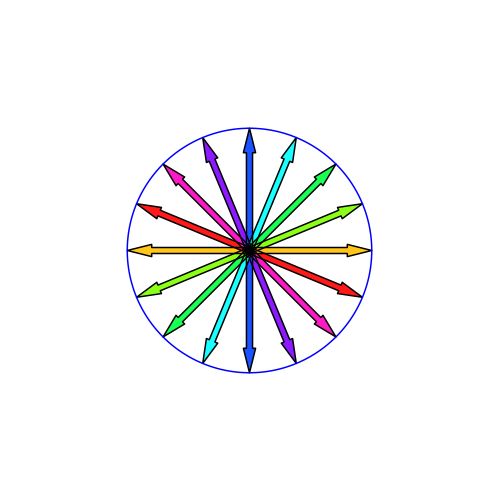
\includegraphics[keepaspectratio]{eigenv1.png}}\end{minipage}%
%
\begin{minipage}{0.50\linewidth}
\pandocbounded{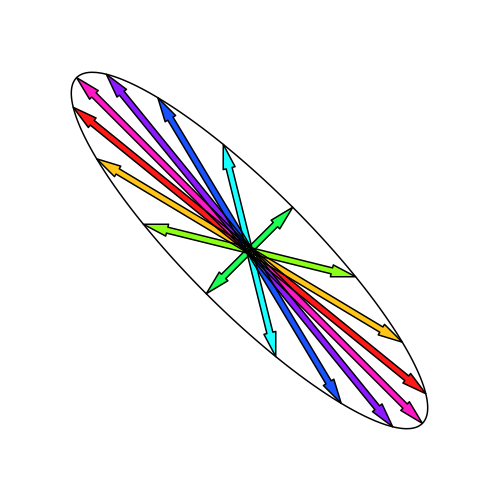
\includegraphics[keepaspectratio]{eigenv2.png}}\end{minipage}%

\caption{\label{fig-deformation}Effect of a deformation on the points
(vectors) in an elastic sphere.}

\end{figure}%

There are some vectors in these plots that don't change direction, but
only their length under the deformation. We can find those by
superimposing the two plots:

\begin{figure}

\begin{minipage}{0.50\linewidth}
\pandocbounded{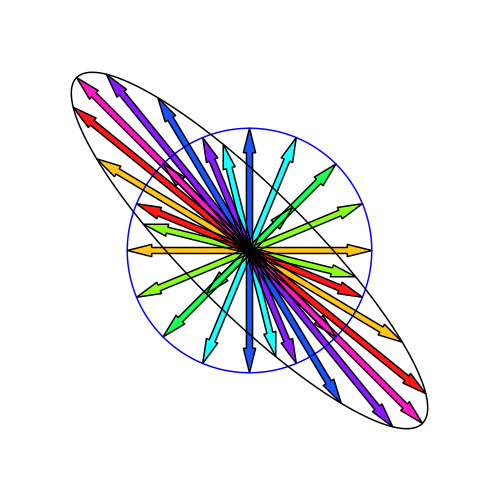
\includegraphics[keepaspectratio]{eigenv3.png}}\end{minipage}%
%
\begin{minipage}{0.50\linewidth}
\pandocbounded{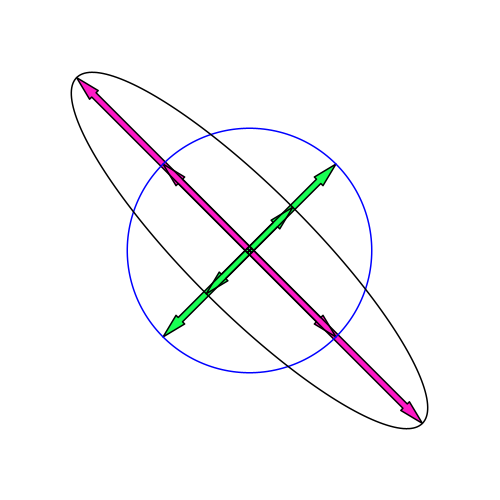
\includegraphics[keepaspectratio]{eigenv4.png}}\end{minipage}%

\caption{\label{fig-deformation2}There are directions in which the
vectors only change their length.}

\end{figure}%

These directions are characteristic of the deformation, as is the factor
of elongation/compression along these directions. These directions can
be found mathematically as the eigenvectors of a matrix, the deformation
matrix, which maps the original vectors to the vectors of the deformed
ball. The eigenvalues are the factors of compression/elongation along
these directions. The word "eigen" is German for "own" and was likely
introduced by David Hilbert (also known for Hilbert spaces).

Eigenvalues and eigenvectors play an essential role in mathematics,
physics and engineering. The stability of an equilibrium of a dynamical
system is determined by the eigenvalues of a matrix that describes the
linearised system at the equilibrium point. The values of a measurement
in quantum mechanics are the eigenvalues of an operator. The principal
axes of a rigid body are the eigenvectors of the moment of inertia
tensor.

\phantomsection\label{eigenvalue-and-eigenvector}
\begin{fbxSimple}{Definition}{Definition 5.1: }{Eigenvalue and Eigenvector}
\phantomsection\label{eigenvalue-and-eigenvector}
Let \(A\) be an \(n \times n\) matrix. A scalar \(\lambda\) is called an
eigenvalue of \(A\) if there is a nonzero vector \(\mathbf{x}\) such
that \(A\mathbf{x} = \lambda \mathbf{x}\). Such a vector \(\mathbf{x}\)
is called an eigenvector of \(A\) corresponding to \(\lambda\).

\end{fbxSimple}

\begin{example}[]\protect\hypertarget{exm-}{}\label{exm-}

Suppose
\(A\left[\begin{array}{c} x \\ y \end{array}\right] = \left[\begin{array}{c} 2x \\ 0 \end{array}\right]\).
Then
\[A\left[\begin{array}{c} 1 \\ 0 \end{array}\right] = \left[\begin{array}{c} 2 \\ 0 \end{array}\right] = 2\left[\begin{array}{c} 1 \\ 0 \end{array}\right]\]
so \(2\) is an eigenvalue and
\(\left[\begin{array}{c} 1 \\ 0 \end{array}\right]\) a corresponding
eigenvector. Also,
\[A\left[\begin{array}{c} 0 \\ 1 \end{array}\right] = \left[\begin{array}{c} 0 \\ 0 \end{array}\right] = 0\left[\begin{array}{c} 0 \\ 1 \end{array}\right],\]
so \(0\) is an eigenvalue and
\(\left[\begin{array}{c} 0 \\ 1 \end{array}\right]\) a corresponding
eigenvector.

\end{example}

Notice that \(\left[\begin{array}{c} \alpha \\ 0 \end{array}\right]\)
and \(\left[\begin{array}{c} 0 \\ \alpha \end{array}\right]\) are
eigenvectors for any \(\alpha \neq 0\).\\
In general, if \(\mathbf{v}\) is an eigenvector of \(A\), then so is
\(\alpha \mathbf{v}\) for any nonzero scalar \(\alpha\).

\begin{example}[]\protect\hypertarget{exm-}{}\label{exm-}

Show that \(5\) is an eigenvalue of
\(A = \left[\begin{array}{cc} 1 & 2 \\ 4 & 3 \end{array}\right]\) and
determine all eigenvectors corresponding to this eigenvalue.

\end{example}

\phantomsection\label{Solutionux2a-5.1}
\begin{fbx}{Solution}{Solution}{}
\phantomsection\label{Solution*-5.1}
We must show that there is a nonzero vector \(\mathbf{x}\) such that
\(A\mathbf{x} = 5\mathbf{x}\), which is equivalent to the equation
\((A - 5I)\mathbf{x} = \mathbf{0}\). We compute the nullspace by:

\[\left[A - 5I | \mathbf{0}\right] = \left[\begin{array}{cc|c} -4 & 2 & 0 \\ 4 & -2 & 0 \end{array}\right] \xrightarrow{R_{2} + R_{1}} \left[\begin{array}{cc|c} -4 & 2 & 0 \\ 0 & 0 & 0 \end{array}\right]\]

Thus
\(\mathbf{x} = \left[\begin{array}{c} x_{1} \\ x_{2} \end{array}\right] \in {\rm Null}(A-5I)\)
satisfies \(-4x_{1} + 2x_{2} = 0\), or \(x_{2} = 2x_{1}\).\\
Thus, \(A\mathbf{x} = 5\mathbf{x}\) has a nontrivial solution of the
form
\(\mathbf{x} = \left[\begin{array}{c} x_{1} \\ x_{2} \end{array}\right] = \left[\begin{array}{c} x_{1} \\ 2x_{1} \end{array}\right] = x_{1}\left[\begin{array}{c} 1 \\ 2 \end{array}\right]\),
so \(5\) is an eigenvalue of \(A\) and the corresponding eigenvectors
are the nonzero multiples of
\(\left[\begin{array}{c} 1 \\ 2 \end{array}\right]\).

\end{fbx}

\phantomsection\label{eigenspace}
\begin{fbxSimple}{Definition}{Definition 5.2: }{Eigenspace}
\phantomsection\label{eigenspace}
Let \(A\) be an \(n \times n\) matrix and let \(\lambda\) be an
eigenvalue of \(A\). The collection of all eigenvectors corresponding to
\(\lambda\), together with the zero vector, is called the eigenspace of
\(\lambda\) and is denoted by \(E_{\lambda }\).

\end{fbxSimple}

Therefore, in the above Example,
\(E_{5} = \left\{t\left[\begin{array}{c} 1 \\ 2 \end{array}\right]\right\}\),
where \(t \in \mathbb{R}\).

\phantomsection\label{characteristic-equation}
\begin{fbxSimple}{Theorem}{Theorem 5.3: }{Characteristic Equation}
\phantomsection\label{characteristic-equation}
Let \(A\) be an \(n \times n\) matrix. Then \(\lambda\) is an eigenvalue
of \(A\) if and only if \(|A-\lambda I_{n}| = 0\) (or
\(det(A - \lambda I_{n}) = 0\)).

\end{fbxSimple}

\phantomsection\label{Proofux2a-5.2}
\begin{fbx}{Proof}{Proof}{}
\phantomsection\label{Proof*-5.2}
Suppose that \(\lambda\) is an eigenvalue of \(A\). Then
\(A\mathbf{v} = \lambda \mathbf{v}\) for some nonzero
\(\mathbf{v} \in \mathbb{R}^{n}\). This is equivalent to
\(A\mathbf{v} = \lambda I_{n} \mathbf{v}\) or
\((A - \lambda I_{n})\mathbf{v} = \mathbf{0}\). But this means that
\(\mathbf{v}\) is a nonzero solution to the homogeneous system of
equations defined by the matrix \(A - \lambda I_{n}\). This means
\(A - \lambda I_{n}\) is singular, and so \(|A - \lambda I_{n}| = 0\).\\
Conversely, if \(|A - \lambda I_{n}| = 0\) then \(A - \lambda I_{n}\) is
singular, and so the system of equations defined by
\(A - \lambda I_{n}\) has nonzero solutions. Hence there exists a
nonzero \(\mathbf{v} \in \mathbb{R}^{n}\) with
\((A - \lambda I_{n})\mathbf{v} = \mathbf{0}\), which is equivalent to
\(A \mathbf{v} = \lambda \mathbf{v}\), and so \(\lambda\) is an
eigenvalue of \(A\).~◻

\end{fbx}

\phantomsection\label{characteristic-equationpolynomial}
\begin{fbxSimple}{Definition}{Definition 5.4: }{Characteristic Equation/Polynomial}
\phantomsection\label{characteristic-equationpolynomial}
For an \(n \times n\) matrix \(A\), the equation
\(|A - \lambda I_{n}| = 0\) is called the characteristic equation of
\(A\), and \(|A - \lambda I_{n}|\) is called the characteristic
polynomial of \(A\).

\end{fbxSimple}

\begin{example}[]\protect\hypertarget{exm-}{}\label{exm-}

Find the eigenvalues and the corresponding eigenvectors of
\(A = \left[\begin{array}{cc}
        1 & 2 \\
        4 & -1
    \end{array}\right]\).

\begin{fbx}{Solution}{Solution}{}
\phantomsection\label{}
The characteristic polynomial is

\[\begin{alignedat}{2}
        |A - \lambda I_{2}| &= \left|\begin{array}{cc}
            1 - \lambda & 2 \\
            4 & -1-\lambda 
        \end{array}\right| \\
        {} &= (1-\lambda )(-1-\lambda ) - 8 \\
        {} &= \lambda ^{2} - 9 \\
        {} &= (\lambda + 3)(\lambda - 3). \\
    \end{alignedat}\] Hence the eigenvalues of \(A\) are the roots of
\((\lambda + 3)(\lambda - 3) = 0\); that is \(\lambda _{1} = -3\) and
\(\lambda _{2} = 3\).\\
To find the eigenvectors corresponding to \(\lambda _{1} = -3\), we find
the nullspace of
\[A - (-3)I_{2} = \left[\begin{array}{cc} 4 & 2 \\ 4 & 2 \end{array}\right]\]

Row reduction produces
\[\left[A+3I_{2} | \mathbf{0}\right] = \left[\begin{array}{cc|c} 4 & 2 & 0 \\ 4 & 2 & 0 \end{array}\right] \xrightarrow{R_{2} - R_{1}} \left[\begin{array}{cc|c} 4 & 2 & 0 \\ 0 & 0 & 0 \end{array}\right]\]

Thus \(\mathbf{x} \in {\rm Null}(A+3I_{2})\) if and only if
\(4x_{1} + 2x_{2} = 0\).\\
Setting the free variable \(x_{2} = t\), we see that
\(x_{1} = -\frac{1}{2}t\). We take
\(\left[\begin{array}{c} x_{1} \\ x_{2} \end{array}\right] = \left[\begin{array}{c} -1 \\ 2 \end{array}\right]\)
be our eigenvector; or indeed any nonzero multiple of
\(\left[\begin{array}{c} -1 \\ 2 \end{array}\right]\).\\
To find the eigenvectors corresponding to \(\lambda _{2} = 3\), we find
the nullspace of \(A - 3I_{2}\) by row reduction:
\[\left[A - 3I_{2} | \mathbf{0}\right] = \left[\begin{array}{cc|c} -2 & 2 & 0 \\ 4 & -4 & 0 \end{array}\right] \xrightarrow{R_{2} + 2R_{1}} \left[\begin{array}{cc|c} -2 & 2 & 0 \\ 0 & 0 & 0 \end{array}\right]\]

So
\(\mathbf{x} = \left[\begin{array}{c} x_{1} \\ x_{2} \end{array}\right] \in {\rm Null}(A - 3I_{2})\)
if and only if \(-2x_{1} + 2x_{2} = 0\). Setting the free variable
\(x_{2} = t\), we find \(x_{1} = t\). We take
\(\left[\begin{array}{c} x_{1} \\ x_{2} \end{array}\right] = \left[\begin{array}{c} 1 \\ 1 \end{array}\right]\)
to be our eigenvector.

\end{fbx}

\end{example}

\begin{example}[]\protect\hypertarget{exm-}{}\label{exm-}

Find the eigenvalues and the corresponding eigenvectors of
\[A = \left[\begin{array}{ccc}
            3 & 2 & 2 \\
            1 & 4 & 1 \\
            -2 & -4 & -1
        \end{array}\right]\].

\end{example}

\phantomsection\label{Solutionux2a-5.3}
\begin{fbx}{Solution}{Solution}{}
\phantomsection\label{Solution*-5.3}
The characteristic equation is \[\begin{alignedat}{2}
        0 = |A - \lambda I| &= \left|\begin{array}{ccc}
            3-\lambda & 2 & 2 \\
            1 & 4-\lambda & 1 \\
            -2 & -4 & -1-\lambda 
        \end{array}\right| \\
        {} &= (3-\lambda ) \left|\begin{array}{cc} 4-\lambda & 1 \\ -4 & -1-\lambda \end{array}\right| - 2 \left|\begin{array}{cc} 1 & 1 \\ -2 & -1-\lambda \end{array}\right| + 2 \left|\begin{array}{cc} 1 & 4-\lambda \\ -2 & -4\end{array}\right| \\
        {} &= (3-\lambda ) \{(4-\lambda )(-1-\lambda )+4\} - 2\{(-1-\lambda )+2\} + 2\{-4+2(4-\lambda )\} \\
        {} &= -\lambda ^3 + 6\lambda ^2 - 11\lambda + 6 \\
        {} &= (\lambda -1)(-\lambda ^2 + 5\lambda - 6) \\
        {} &= (\lambda -1)\{-(\lambda ^2 - 5\lambda + 6)\} \\
        {} &= (\lambda -1)\{-(\lambda - 2)(\lambda - 3)\} \\
    \end{alignedat}\]

Hence, the eigenvalues are \(\lambda _{1} = 1, \lambda _{2} = 2\) and
\(\lambda _{3} = 3\).\\
For \(\lambda _{1}=1\), we compute
\[\left[A - I | \mathbf{0}\right] = \left[\begin{array}{ccc | c} \textcircled{\raisebox{-0.9pt}{2}} & 2 & 2 & 0 \\ 1 & 3 & 1 & 0 \\ -2 & -4 & -2 & 0 \end{array}\right] \xrightarrow{\begin{subarray}{c} R_{2} - \frac{1}{2}R_{1} \\ R_{3} + R_{1} \end{subarray}} \left[\begin{array}{ccc | c} 2 & 2 & 2 & 0 \\ 0 & \textcircled{\raisebox{-0.9pt}{2}} & 0 & 0 \\ 0 & -2 & 0 & 0 \end{array}\right] \]
\[\xrightarrow{R_{3} + R_{2}} \left[\begin{array}{ccc | c} \textcircled{\raisebox{-0.9pt}{2}} & 2 & 2 & 0 \\ 0 & \textcircled{\raisebox{-0.9pt}{2}} & 0 & 0 \\ 0 & 0 & 0 & 0 \end{array}\right]\]
from which it follows that an eigenvector
\[\mathbf{x} = \left[\begin{array}{c} x_{1} \\ x_{2} \\ x_{3} \end{array}\right]\]
satisfies \(x_{2} = 0\) and \(x_{3} = -x_{1}\). We take
\(\left[\begin{array}{c} x_{1} \\ x_{2} \\ x_{3} \end{array}\right] = \left[\begin{array}{c} 1 \\ 0 \\ -1 \end{array}\right]\)
to be our eigenvector .

For \(\lambda _{2} = 2\), we compute
\[\left[A - 2I | \mathbf{0}\right] = \left[\begin{array}{ccc | c} \textcircled{\raisebox{-0.9pt}{1}} & 2 & 2 & 0 \\ 1 & 2 & 1 & 0 \\ -2 & -4 & -3 & 0 \end{array}\right] \xrightarrow{\begin{subarray}{c} R_{2} - R_{1} \\ R_{3} + 2R_{1} \end{subarray}} \left[\begin{array}{ccc | c} 1 & 2 & 2 & 0 \\ 0 & 0 & \textcircled{\raisebox{-0.9pt}{-1}} & 0 \\ 0 & 0 & 3 & 0 \end{array}\right]\]
\[\xrightarrow{R_{3} + 3R_{2}} \left[\begin{array}{ccc | c} \textcircled{\raisebox{-0.9pt}{1}} & 2 & 2 & 0 \\ 0 & 0 & \textcircled{\raisebox{-0.9pt}{-1}} & 0 \\ 0 & 0 & 0 & 0 \end{array}\right]\]
which gives an eigenvector
\[\mathbf{x} = \left[\begin{array}{c} -2 \\ 1 \\ 0 \end{array}\right]\].

For \(\lambda _{3} = 3\), we compute
\[\left[A - 3I | \mathbf{0}\right] = \left[\begin{array}{ccc | c} 0 & 2 & 2 & 0 \\ 1 & 1 & 1 & 0 \\ -2 & -4 & -4 & 0 \end{array}\right] \xrightarrow{R_{2} \leftrightarrow R_{1}} \left[\begin{array}{ccc | c} \textcircled{\raisebox{-0.9pt}{1}} & 1 & 1 & 0 \\ 0 & 2 & 2 & 0 \\ -2 & -4 & -4 & 0 \end{array}\right] \]
\[\xrightarrow{R_{3} + 2R_{1}} \left[\begin{array}{ccc | c} 1 & 1 & 1 & 0 \\ 0 & \textcircled{\raisebox{-0.9pt}{2}} & 2 & 0 \\ 0 & -2 & -2 & 0 \end{array}\right] \xrightarrow{R_{3} + R_{2}} \left[\begin{array}{ccc | c} 1 & 1 & 1 & 0 \\ 0 & 2 & 2 & 0 \\ 0 & 0 & 0 & 0 \end{array}\right]\]
which gives an eigenvector
\[\mathbf{x} = \left[\begin{array}{c} 0 \\ -1 \\ 1 \end{array}\right]\].

\end{fbx}

\begin{example}[]\protect\hypertarget{exm-}{}\label{exm-}

Find the eigenvalues and the corresponding eigenspaces of
\[A = \left[\begin{array}{ccc}
        0 & 1 & 0 \\
        0 & 0 & 1 \\
        2 & -5 & 4
    \end{array}\right]\]

\end{example}

\phantomsection\label{Solutionux2a-5.4}
\begin{fbx}{Solution}{Solution}{}
\phantomsection\label{Solution*-5.4}
The characteristic equations is

\[\begin{alignedat}{2}
        0 = |A - \lambda I| &= \left|\begin{array}{ccc}
            -\lambda & 1 & 0 \\
            0 & -\lambda & 1 \\
            2 & -5 & 4-\lambda 
        \end{array}\right| \\
        {} &= -\lambda \left|\begin{array}{cc} -\lambda & 1 \\ -5 & 4-\lambda \end{array}\right| -  \left|\begin{array}{cc} 0 & 1 \\ 2 & 4-\lambda \end{array}\right| \\
        {} &= -\lambda (\lambda ^2-4\lambda +5)-(-2) \\
        {} &= -\lambda ^3 + 4\lambda ^2 - 5\lambda + 2 \\
        {} &= (\lambda -1)(-\lambda ^2 + 3\lambda - 2) \\
        {} &= -(\lambda -1)^2(\lambda -2) \\
    \end{alignedat}\]

Hence, the eigenvalues are \(\lambda _{1} = \lambda _{2} = 1\) and
\(\lambda _{3} = 2\).\\
To find the eigenvectors corresponding to
\(\lambda _{1} = \lambda _{2} = 1\), we compute
\[\left[A - I | \mathbf{0}\right] = \left[\begin{array}{ccc | c} \textcircled{\raisebox{-0.9pt}{-1}} & 1 & 0 & 0 \\ 0 & -1 & 1 & 0 \\ 2 & -5 & 3 & 0 \end{array}\right] \xrightarrow{R_{3} + 2R_{1}} \left[\begin{array}{ccc | c} -1 & 1 & 0 & 0 \\ 0 & \textcircled{\raisebox{-0.9pt}{-1}} & 1 & 0 \\ 0 & -3 & 3 & 0 \end{array}\right] \xrightarrow{R_{3} - 3R_{2}} \left[\begin{array}{ccc | c} -1 & 1 & 0 & 0 \\ 0 & -1 & 1 & 0 \\ 0 & 0 & 0 & 0 \end{array}\right]\]

Thus,
\[\mathbf{x} = \left[\begin{array}{c} x_{1} \\ x_{2} \\ x_{3} \end{array}\right]\]
is in the eigenspace \(E_{1}\) if and only if \(-x_{1} + x_{2} = 0\) and
\(-x_{2} + x_{3} = 0\). Setting the free variable \(x_{3} = t\), we see
that \(x_{1} = t\) and \(x_{2} = t\), from which it follows that
\[E_{1} = \left\{\left[\begin{array}{c} t \\ t \\ t \end{array}\right]\right\} = \left\{t \left[\begin{array}{c} 1 \\ 1 \\ 1 \end{array}\right]\right\} = {\rm span}\left(\left[\begin{array}{c} 1 \\ 1 \\ 1 \end{array}\right]\right)\]

To find the eigenvectors correspond to \(\lambda _{3} = 2\), we find the
nullspace of \(A - 2I\) by row reduction:
\[\left[A - 2I | \mathbf{0}\right] = \left[\begin{array}{ccc | c} \textcircled{\raisebox{-0.9pt}{-2}} & 1 & 0 & 0 \\ 0 & -2 & 1 & 0 \\ 2 & -5 & 2 & 0 \end{array}\right] \xrightarrow{R_{3} + R_{1}} \left[\begin{array}{ccc | c} -2 & 1 & 0 & 0 \\ 0 & \textcircled{\raisebox{-0.9pt}{-2}} & 1 & 0 \\ 0 & -4 & 2 & 0 \end{array}\right] \]
\[\xrightarrow{R_{3} - 2R_{2}} \left[\begin{array}{ccc | c} -2 & 1 & 0 & 0 \\ 0 & -2 & 1 & 0 \\ 0 & 0 & 0 & 0 \end{array}\right]\]

So
\[\mathbf{x} = \left[\begin{array}{c} x_{1} \\ x_{2} \\ x_{3} \end{array}\right]\]
is in the eigenspace \(E_{2}\) if and only if \(-2x_{1} + x_{2} = 0\)
and \(-2x_{2} + x_{3} = 0\). Setting the free variable \(x_{3} = t\), we
have
\[E_{2} = \left\{\left[\begin{array}{c} \frac{1}{4}t \\ \frac{1}{2}t \\ t \end{array}\right]\right\} = \left\{t \left[\begin{array}{c} \frac{1}{4} \\ \frac{1}{2} \\ 1 \end{array}\right]\right\} = {\rm span}\left(\left[\begin{array}{c} \frac{1}{4} \\ \frac{1}{2} \\ 1 \end{array}\right]\right) = {\rm span}\left(\left[\begin{array}{c} 1 \\ 2 \\ 4 \end{array}\right]\right)\]

\end{fbx}

\phantomsection\label{algebraic-and-geometric-multiplicity}
\begin{fbxSimple}{Definition}{Definition 5.5: }{Algebraic and Geometric Multiplicity}
\phantomsection\label{algebraic-and-geometric-multiplicity}
The algebraic multiplicity of an eigenvalue is its multiplicity as a
root of the characteristic equation.\\
The geometric multiplicity of an eigenvalue \(\lambda\) is
\({\rm dim} (E_{\lambda })\), the dimension of its corresponding
eigenspace.

\end{fbxSimple}

In the above Example, \(\lambda = 1\) has algebraic multiplicity \(2\)
and geometric multiplicity \(1\). \(\lambda = 2\) has algebraic
multiplicity \(1\) and geometric multiplicity \(1\).

\phantomsection\label{eigenvaluestriangular}
\begin{fbxSimple}{Corollary}{Corollary 5.6}{}
\phantomsection\label{eigenvaluestriangular}
The eigenvalues of a triangular matrix are the entries on its main
diagonal.

\end{fbxSimple}

\begin{example}[]\protect\hypertarget{exm-}{}\label{exm-}

Let
\[A = \left[\begin{array}{cccc} 2 & 0 & 0 & 0 \\ -1 & 1 & 0 & 0 \\ 3 & 0 & 3 & 0 \\ 5 & 7 & 4 & -2 \end{array}\right]\]
The characteristic polynomial is: \[\begin{alignedat}{2}
        |A - \lambda I| &= \left|\begin{array}{cccc} 2-\lambda & 0 & 0 & 0 \\ -1 & 1-\lambda & 0 & 0 \\ 3 & 0 & 3-\lambda & 0 \\ 5 & 7 & 4 & -2-\lambda \end{array}\right| \\
        {} &= (2-\lambda )\left|\begin{array}{ccc} 1-\lambda & 0 & 0 \\ 0 & 3-\lambda & 0 \\ 7 & 4 & -2-\lambda \end{array}\right| \\
        {} &= (2-\lambda )(1-\lambda )\left|\begin{array}{cc} 3-\lambda & 0 \\ 4 & -2-\lambda \end{array}\right| \\
        {} &= (2-\lambda )(1-\lambda )(3-\lambda )(-2-\lambda ) 
    \end{alignedat}\]

Hence, the eigenvalues are
\(\lambda _{1}=2, \lambda _{2}=1, \lambda _{3}=3, \lambda _{4}=-2\).

\end{example}

Note that diagonal matrices are a special case of Corollary
\hyperref[eigenvaluestriangular]{5.6}.

\phantomsection\label{eigenlinind}
\begin{fbxSimple}{Theorem}{Theorem 5.7}{}
\phantomsection\label{eigenlinind}
Let \(A\) be an \(n \times n\) matrix and let
\(\lambda _{1}, \lambda _{2}, ..., \lambda _{m}\) be distinct
eigenvalues of \(A\) with corresponding eigenvectors
\(\mathbf{v_{1}}, \mathbf{v_{2}}, ..., \mathbf{v_{m}}\). Then
\(\mathbf{v_{1}}, \mathbf{v_{2}}, ..., \mathbf{v_{m}}\) are linearly
independent.

\end{fbxSimple}

\phantomsection\label{Proofux2a-5.5}
\begin{fbx}{Proof}{Proof}{}
\phantomsection\label{Proof*-5.5}
We prove this by contradiction.

Suppose \(\mathbf{v_{1}}, \mathbf{v_{2}}, ..., \mathbf{v_{m}}\) are
linearly dependent. Let \(\mathbf{v_{k+1}}\) be the first of the vectors
\(\mathbf{v_{i}}\) that can be expressed as a linear combination of the
previous ones. In other words,
\(\mathbf{v_{1}}, \mathbf{v_{2}}, ..., \mathbf{v_{k}}\) are linearly
independent, but there are \(c_{1}, c_{2}, ..., c_{k}\) such that
\[\mathbf{v_{k+1}} = c_{1}\mathbf{v_{1}} + c_{2}\mathbf{v_{2}} + ... + c_{k}\mathbf{v_{k}} \qquad (1)\]

Multiplying both sides of Equation (1) by \(A\) from left and using the
fact that \(A\mathbf{v_{i}} = \lambda _{i}\mathbf{v_{i}}\) for each
\(i\), we have \[\begin{alignedat}{2}
        \lambda _{k+1}\mathbf{v_{k+1}} = A\mathbf{v_{k+1}} &= A(c_{1}\mathbf{v_{1}} + c_{2}\mathbf{v_{2}} + ... + c_{k}\mathbf{v_{k}}) \\
        {} &= c_{1}A\mathbf{v_{1}} + c_{2}A\mathbf{v_{2}} + ... + c_{k}A\mathbf{v_{k}} \\
        {} &= c_{1}\lambda _{1}\mathbf{v_{1}} + c_{2}\lambda _{2}\mathbf{v_{2}} + ... + c_{k}\lambda _{k}\mathbf{v_{k}} \qquad (2) 
    \end{alignedat}\]

Now we multiply both sides of Equation (1) by \(\lambda _{k+1}\) to
obtain
\[\lambda _{k+1}\mathbf{v_{k+1}} = c_{1}\lambda _{k+1}\mathbf{v_{1}} + c_{2}\lambda _{k+1}\mathbf{v_{2}} + ... + c_{k}\lambda _{k+1}\mathbf{v_{k}} \qquad (3)\]

When we subtract Equation (3) from Equation (2), we obtain
\[\mathbf{0} = c_{1}(\lambda _{1}-\lambda _{k+1})\mathbf{v_{1}} + c_{2}(\lambda _{2}-\lambda _{k+1})\mathbf{v_{2}} + ... + c_{k}(\lambda _{k}-\lambda _{k+1})\mathbf{v_{k}}\]

The linear independence of
\[\mathbf{v_{1}}, \mathbf{v_{2}}, ..., \mathbf{v_{k}}\] implies that
\[c_{1}(\lambda _{1}-\lambda _{k+1}) = c_{2}(\lambda _{2}-\lambda _{k+1}) = ... = c_{k}(\lambda _{k}-\lambda _{k+1}) = 0\]

Since the eigenvalues \(\lambda _{i}\) are all distinct,
\(\lambda _{i} - \lambda _{k+1} \neq 0\) for all \(i = 1, ..., k\).
Hence \(c_{1} = c_{2} = ... = c_{k} = 0\). This implies that
\[\mathbf{v_{k+1}} = 0\mathbf{v_{1}} + 0\mathbf{v_{2}} + ... + 0\mathbf{v_{k}} = \mathbf{0}\]

which is impossible since the eigenvector \(\mathbf{v_{k+1}}\) cannot be
zero.

Thus, our assumption that
\(\mathbf{v_{1}}, \mathbf{v_{2}}, ..., \mathbf{v_{m}}\) are linearly
dependent is false. It follows that
\(\mathbf{v_{1}}, \mathbf{v_{2}}, ..., \mathbf{v_{m}}\) must be linearly
independent.~◻

\end{fbx}

\section{Similarity and
Diagonalisation}\label{similarity-and-diagonalisation}

\subsection{Introduction}\label{introduction-2}

In many applications, matrices represent linear mappings of vectors in a
physical space, as in the example given at the start of the Eigenvector
section. The choice of a coordinate system (in particular, its
orientation) in this space is arbitrary, and this choice determines what
the matrix looks like. In this section, we show that under certain
conditions, there exists a choice of a coordinate system in which the
matrix becomes a diagonal matrix. In this case, the coordinate axes have
the direction of the eigenvectors of the matrix, and the diagonal
elements of the matrix are the eigenvalues.

\subsection{Similar Matrices}\label{similar-matrices}

\phantomsection\label{similar-matrices-1}
\begin{fbxSimple}{Definition}{Definition 5.8: }{Similar Matrices}
\phantomsection\label{similar-matrices-1}
Let \(A\) and \(B\) be \(n \times n\) matrices. We say that \(A\) is
similar to \(B\) if there is an invertible \(n \times n\) matrix \(P\)
such that \(P^{-1}AP = B\). If \(A\) is similar to \(B\), we write
\(A \sim B\).

\end{fbxSimple}

\begin{tcolorbox}[enhanced jigsaw, colback=white, leftrule=.75mm, title=\textcolor{quarto-callout-note-color}{\faInfo}\hspace{0.5em}{Remark}, toprule=.15mm, toptitle=1mm, titlerule=0mm, bottomrule=.15mm, opacitybacktitle=0.6, bottomtitle=1mm, coltitle=black, arc=.35mm, opacityback=0, breakable, colframe=quarto-callout-note-color-frame, rightrule=.15mm, left=2mm, colbacktitle=quarto-callout-note-color!10!white]

If \(A \sim B\), we can write, equivalently, that \(A = PBP^{-1}\) or
\(AP = PB\). The matrix \(P\) depends on \(A\) and \(B\). It is not
unique for a given pair of similar matrices \(A\) and \(B\).

\end{tcolorbox}

\phantomsection\label{simmatrices}
\begin{fbxSimple}{Theorem}{Theorem 5.9: }{Properties of Similar Matrices}
\phantomsection\label{simmatrices}
Let \(A\) and \(B\) be \(n \times n\) matrices with \(A \sim B\). Then\\
(a) \(det(A) = det(B)\)\\
(b) \(A\) and \(B\) have the same rank.\\
(c) \(A\) and \(B\) have the same characteristic polynomial.\\
(d) \(A\) and \(B\) have the same eigenvalues.

\end{fbxSimple}

\phantomsection\label{Proofux2a-5.6}
\begin{fbx}{Proof}{Proof}{}
\phantomsection\label{Proof*-5.6}
If \(A \sim B\), then \(P^{-1}AP = B\) for some invertible matrix
\(P\).\\
(a)\\
\[\begin{alignedat}{2}
            \qquad det(B) &= det(P^{-1}AP) \\
            {} &= det(P^{-1})det(A)det(P) \\
            {} &= \frac{1}{det(P)}det(A)det(P) \\
            {} &= det(A). \\
        \end{alignedat}\]

(c) The characteristic polynomial of \(B\) is \[\begin{alignedat}{2}
            det(B - \lambda I) &= det(P^{-1}AP - \lambda I) \\
            {} &= det(P^{-1}AP - \lambda P^{-1}IP) \\
            {} &= det(P^{-1}AP - P^{-1}(\lambda I)P) \\
            {} &= det(P^{-1}(A - \lambda I)P) \\
            {} &= det(P^{-1})det(A - \lambda I)det(P) \\
            {} &= \frac{1}{det(P)}det(A - \lambda I)det(P) \\
            {} &= det(A - \lambda I)  
        \end{alignedat}\] ~◻

\end{fbx}

Theorem \hyperref[simmatrices]{5.9} is helpful in showing that two
matrices are not similar, since \(A\) and \(B\) cannot be similar if any
of the properties fail.

\begin{example}[]\protect\hypertarget{exm-}{}\label{exm-}

~

\begin{enumerate}
\def\labelenumi{(\alph{enumi})}
\tightlist
\item
  The two matrices
  \[A = \left[\begin{array}{cc} 1 & 2 \\ 2 & 1 \end{array}\right], \quad B = \left[\begin{array}{cc} 2 & 1 \\ 1 & 2 \end{array}\right], \]
  are not similar since \(det(A) = -3\) but \(det(B) = 3\).\\
\item
  The two matrices
  \[A = \left[\begin{array}{cc} 1 & 3 \\ 2 & 2 \end{array}\right], \quad B = \left[\begin{array}{cc} 1 & 1 \\ 3 & -1 \end{array}\right]\]
  are not similar, since
  \(|A - \lambda I| = \lambda ^{2} - 3\lambda - 4\) while
  \(|B - \lambda I| = \lambda ^{2} - 4\). Note that \(A\) and \(B\) have
  the same determinant and rank, however.
\end{enumerate}

\end{example}

\subsection{Diagonalisation}\label{diagonalisation}

\phantomsection\label{diagonalisable-matrices}
\begin{fbxSimple}{Definition}{Definition 5.10: }{Diagonalisable Matrices}
\phantomsection\label{diagonalisable-matrices}
An \(n \times n\) matrix \(A\) is diagonalisable if there is a diagonal
matrix \(D\) such that \(A\) is similar to \(D\) - that is, if there is
an invertible \(n \times n\) matrix \(P\) such that \(P^{-1}AP = D\).

\end{fbxSimple}

\phantomsection\label{diagifind}
\begin{fbxSimple}{Theorem}{Theorem 5.11: }{Condition for Diagonalisability}
\phantomsection\label{diagifind}
Let \(A\) be an \(n \times n\) matrix. Then \(A\) is diagonalisable if
and only if \(A\) has \(n\) linearly independent eigenvectors.\\
More precisely, there exists an invertible matrix \(P\) and a diagonal
matrix \(D\) such that \(P^{-1}AP = D\) if and only if the columns of
\(P\) are \(n\) linearly independent eigenvectors of \(A\) and the
diagonal entries of \(D\) are the eigenvalues of \(A\) corresponding to
the eigenvectors in \(P\) in the same order.*

\end{fbxSimple}

\phantomsection\label{Proofux2a-5.7}
\begin{fbx}{Proof}{Proof}{}
\phantomsection\label{Proof*-5.7}
Suppose first that \(A\) is similar to the diagonal matrix \(D\) by
\(P^{-1}AP = D\) or, equivalently, \(AP = PD\). Let the columns of \(P\)
be \(\mathbf{p_{1}}, \mathbf{p_{2}}, ..., \mathbf{p_{n}}\) and let the
diagonal entries of \(D\) be
\(\lambda _{1}, \lambda _{2}, ..., \lambda _{n}\). Then
\[A\left[\mathbf{p_{1}}, \mathbf{p_{2}}, \cdots, \mathbf{p_{n}}\right] = \left[\mathbf{p_{1}}, \mathbf{p_{2}}, \cdots, \mathbf{p_{n}}\right] \left[\begin{array}{cccc} \lambda _{1} & 0 & \cdots & 0 \\ 0 & \lambda _{2} & \cdots & 0 \\ \vdots & \vdots & \ddots & \vdots \\ 0 & 0 & \cdots & \lambda _{n} \end{array}\right] \qquad (1)\]
or
\[\qquad \left[A\mathbf{p_{1}}, A\mathbf{p_{2}}, \cdots, A\mathbf{p_{n}}\right] = \left[\lambda _{1}\mathbf{p_{1}}, \lambda _{2}\mathbf{p_{2}}, \cdots, \lambda _{n}\mathbf{p_{n}}\right] \qquad (2)\]

Equating columns, we have
\[A\mathbf{p_{1}} = \lambda _{1}\mathbf{p_{1}}, A\mathbf{p_{2}} = \lambda _{2}\mathbf{p_{2}}, \cdots , A\mathbf{p_{n}} = \lambda _{n}\mathbf{p_{n}}\]
which proves that the column vectors of \(P\) are eigenvectors of \(A\)
whose corresponding eigenvalues are the diagonal entries of \(D\) in the
same order. Since \(P\) is invertible, its columns are linearly
independent.

Conversely, if \(A\) has \(n\) linearly independent eigenvectors
\(\mathbf{p_{1}}, \mathbf{p_{2}}, \cdots , \mathbf{p_{n}}\) with
corresponding eigenvalues
\(\lambda _{1}, \lambda _{2}, \cdots , \lambda _{n}\), respectively,
then
\[A\mathbf{p_{1}} = \lambda _{1}\mathbf{p_{1}}, A\mathbf{p_{2}} = \lambda _{2}\mathbf{p_{2}}, \cdots , A\mathbf{p_{n}} = \lambda _{n}\mathbf{p_{n}}\]

This implies Eq. (2), which is equivalent to Eq. (1), that is
\(AP = PD\). Since the columns
\(\mathbf{p_{1}}, \mathbf{p_{2}}, \cdots , \mathbf{p_{n}}\) of \(P\) are
linearly independent, \(P\) is invertible, so \(P^{-1}AP = D\), that is,
\(A\) is diagonalisable.~◻

\end{fbx}

\begin{example}[]\protect\hypertarget{exm-}{}\label{exm-}

If possible, find a matrix \(P\) that diagonalises
\[A = \left[\begin{array}{ccc}
            0 & 1 & 0 \\
            0 & 0 & 1 \\
            2 & -5 & 4 
        \end{array}\right]\]

\end{example}

\phantomsection\label{Solutionux2a-5.8}
\begin{fbx}{Solution}{Solution}{}
\phantomsection\label{Solution*-5.8}
We studied this matrix previously and found that it has eigenvalues
\(\lambda _{1} = \lambda _{2} = 1\) and \(\lambda _{3} = 2\). The
eigenspaces have the following bases:\\
For \(\lambda _{1} = \lambda _{2} = 1\), \(E_{1}\) has basis
\(\left[\begin{array}{c} 1 \\ 1 \\ 1 \end{array}\right]\).\\
For \(\lambda _{3} = 2\), \(E_{2}\) has basis
\(\left[\begin{array}{c} 1 \\ 2 \\ 4 \end{array}\right]\).\\
Since all other eigenvectors are just multiples of one of these two
basis vectors, there cannot be three linearly independent eigenvectors.
By Theorem 4.6, \(A\) is not diagonalisable.

\end{fbx}

\begin{example}[]\protect\hypertarget{exm-}{}\label{exm-}

If possible, find a matrix \(P\) that diagonalises
\[A = \left[\begin{array}{ccc}
            2 & 2 & 0 \\
            0 & 1 & 0 \\
            -4 & -8 & 1 
        \end{array}\right]\]

\end{example}

\phantomsection\label{Solutionux2a-5.9}
\begin{fbx}{Solution}{Solution}{}
\phantomsection\label{Solution*-5.9}
This is the matrix of Question 3, Worksheet 6. There we found that the
eigenvalues of \(A\) are \(\lambda _{1} = 2\) and
\(\lambda _{2} = \lambda _{3} = 1\), with the following bases for the
eigenspaces:\\
For \(\lambda _{1} = 2\), \(E_{2}\) has basis
\(\mathbf{p_{1}} = \left[\begin{array}{c} 1 \\ 0 \\ -4 \end{array}\right]\).\\
For \(\lambda _{2} = \lambda _{3} = 1\), \(E_{1}\) has basis
\(\mathbf{p_{2}} = \left[\begin{array}{c} -2 \\ 1 \\ 0 \end{array}\right]\)
and
\(\mathbf{p_{3}} = \left[\begin{array}{c} 0 \\ 0 \\ 1 \end{array}\right]\).\\
Now we check whether
\(\left\{\mathbf{p_{1}}, \mathbf{p_{2}}, \mathbf{p_{3}}\right\}\) is
linearly independent.
\[\left[\begin{array}{ccc} \textcircled{\raisebox{-0.9pt}{1}} & -2 & 0 \\ 0 & 1 & 0 \\ -4 & 0 & 1 \end{array}\right] \xrightarrow{R_{3} + 4R_{1}} \left[\begin{array}{ccc} 1 & -2 & 0 \\ 0 & \textcircled{\raisebox{-0.9pt}{1}} & 0 \\ 0 & -8 & 1 \end{array}\right] \xrightarrow{R_{3} + 8R_{2}} \left[\begin{array}{ccc} 1 & -2 & 0 \\ 0 & 1 & 0 \\ 0 & 0 & 1 \end{array}\right]\]

Since \(rank = 3\),
\(\left\{\mathbf{p_{1}}, \mathbf{p_{2}}, \mathbf{p_{3}}\right\}\) is
linearly independent. Thus, if we take
\[P = \left[\mathbf{p_{1}}, \mathbf{p_{2}}, \mathbf{p_{3}}\right] = \left[\begin{array}{ccc} 1 & -2 & 0 \\ 0 & 1 & 0 \\ -4 & 0 & 1 \end{array}\right]\]
then \(P\) is invertible. Furthermore,
\[P^{-1}AP = \left[\begin{array}{ccc} 2 & 0 & 0 \\ 0 & 1 & 0 \\ 0 & 0 & 1 \end{array}\right] = D\]

(Note: It is much easier to check the equivalent equation \(AP = PD\)).

\end{fbx}

\begin{tcolorbox}[enhanced jigsaw, colback=white, leftrule=.75mm, title=\textcolor{quarto-callout-note-color}{\faInfo}\hspace{0.5em}{Remark}, toprule=.15mm, toptitle=1mm, titlerule=0mm, bottomrule=.15mm, opacitybacktitle=0.6, bottomtitle=1mm, coltitle=black, arc=.35mm, opacityback=0, breakable, colframe=quarto-callout-note-color-frame, rightrule=.15mm, left=2mm, colbacktitle=quarto-callout-note-color!10!white]

Eigenvectors can be placed into the columns of \(P\) in any order.
However, the eigenvalues will come up on the diagonal of \(D\) in the
same order as their corresponding eigenvectors in \(P\). For example, if
we had chosen
\[P = \left[\mathbf{p_{2}}, \mathbf{p_{3}}, \mathbf{p_{1}}\right] = \left[\begin{array}{ccc} -2 & 0 & 1 \\ 1 & 0 & 0 \\ 0 & 1 & -4 \end{array}\right]\]
Then we would have found
\[P^{-1}AP = \left[\begin{array}{ccc} 1 & 0 & 0 \\ 0 & 1 & 0 \\ 0 & 0 & 2 \end{array}\right]\]

We checked that the eigenvectors \(\mathbf{p_{1}}, \mathbf{p_{2}}\) and
\(\mathbf{p_{3}}\) were linearly independent. However, the following
Theorem guarantees that linear independence is preserved when the bases
of different subspaces are combined.

\end{tcolorbox}

\phantomsection\label{section}
\begin{fbxSimple}{Theorem}{Theorem 5.12}{}
\phantomsection\label{section}
Let \(A\) be an \(n \times n\) matrix and let
\(\lambda _{1}, \lambda _{2}, \cdots, \lambda _{k}\) be distinct
eigenvalues of \(A\). If \(B_{i}\) is a basis for the eigenspace
\(E_{i}\), then \(B = B_{1} \cup B_{2} \cup \cdots \cup B_{k}\)
(i.e.~the total collection of basis vectors for all of the eigenspaces)
is linearly independent.

\end{fbxSimple}

\phantomsection\label{eigendiag}
\begin{fbxSimple}{Theorem}{Theorem 5.13}{}
\phantomsection\label{eigendiag}
If \(A\) is an \(n \times n\) matrix with \(n\) distinct eigenvalues,
then \(A\) is diagonalisable.

\end{fbxSimple}

\phantomsection\label{Proofux2a-5.10}
\begin{fbx}{Proof}{Proof}{}
\phantomsection\label{Proof*-5.10}
Let \(\mathbf{v_{1}}, \mathbf{v_{2}}, \cdots, \mathbf{v_{n}}\) be
eigenvectors corresponding to the \(n\) distinct eigenvalues of \(A\).
By theorem \hyperref[eigenlinind]{5.7},
\(\mathbf{v_{1}}, \mathbf{v_{2}}, \cdots, \mathbf{v_{n}}\) are linearly
independent, so, by Theorem \hyperref[diagifind]{5.11}, \(A\) is
diagonalisable.~◻

\end{fbx}

\begin{example}[]\protect\hypertarget{exm-}{}\label{exm-}

The matrix \[A = \left[\begin{array}{cccc}
            2 & 0 & 0 & 0 \\
            -1 & 1 & 0 & 0 \\
            3 & 0 & 3 & 0 \\
            5 & 7 & 4 & -2
        \end{array}\right]\] has eigenvalues
\(\lambda _{1} = 2, \lambda _{2} = 1, \lambda _{3} = 3\) and
\(\lambda _{4} = -2\), by Corollary
\hyperref[eigenvaluestriangular]{5.6}. Since these are four distinct
eigenvalues for a \(4 \times 4\) matrix, \(A\) is diagonalisable, by
Theorem \hyperref[eigendiag]{5.13}.

\end{example}

\phantomsection\label{Corollary-5.14}
\begin{fbxSimple}{Corollary}{Corollary 5.14}{}
\phantomsection\label{Corollary-5.14}
If \(A\) is an \(n \times n\) matrix, then the geometric multiplicity of
each eigenvalue is less than or equal to its algebraic multiplicity.

\end{fbxSimple}

\phantomsection\label{diagonalisation-theorem}
\begin{fbxSimple}{Theorem}{Theorem 5.15: }{Diagonalisation Theorem}
\phantomsection\label{diagonalisation-theorem}

Let \(A\) be an \(n \times n\) matrix whose distinct eigenvalues are
\(\lambda _{1}, \lambda _{2}, \cdots, \lambda _{k}\), where
\(1\leq k\leq n\). The following statements are equivalent:

\begin{enumerate}
\def\labelenumi{(\alph{enumi})}
\item
  \(A\) is diagonalisable.
\item
  The union \(B\) of the bases of the eigenspaces of \(A\) contains
  \(n\) vectors.
\item
  The algebraic multiplicity of each eigenvalue equals its geometric
  multiplicity.
\end{enumerate}

\end{fbxSimple}

\begin{example}[]\protect\hypertarget{exm-}{}\label{exm-}

~

\begin{enumerate}
\def\labelenumi{(\alph{enumi})}
\tightlist
\item
  The matrix \[A = \left[\begin{array}{ccc}
      0 & 1 & 0 \\ 0 & 0 & 1 \\ 2 & -5 & 4 \end{array}\right]\] has two
  distinct eigenvalues \(\lambda _{1} = \lambda _{2} = 1\) and
  \(\lambda _{3} = 2\). Since the eigenvalue
  \(\lambda _{1} = \lambda _{2} = 1\) with
  \(E_{1} = {\rm span}( (1,1,1)^T)\) has algebraic multiplicity 2 but
  geometric multiplicity 1, \(A\) is not diagonalisable, by the
  Diagonalisation Theorem.\\
\item
  The matrix \[A = \left[\begin{array}{ccc}
      2 & 2 & 0 \\ 0 & 1 & 0 \\ -4 & -8 & 1 \end{array}\right]\] has two
  distinct eigenvalues \(\lambda _{1} = 2\) and
  \(\lambda _{2} = \lambda _{3} = 1\). We found: for
  \(\lambda _{1} = 2\), \(E_{1}\) has basis
  \(\mathbf{p_{1}} = (1, 0, -4)^T\), and for
  \(\lambda _{2} = \lambda _{3} = 1\), \(E_{2}\) has basis
  \(\mathbf{p_{2}} = (-2,1, 0)^T\) and \(\mathbf{p_{3}} = (0,0,1)^T\).
  Thus, the eigenvalue 2 has algebraic and geometric multiplicity 1, and
  the eigenvalue 1 has algebraic and geometric multiplicity 2. Thus,
  \(A\) is diagonalisable, by the Diagonalisation Theorem.
\end{enumerate}

\end{example}

\chapter{Appendix}\label{appendix}

\section{Greek Letters}\label{sec-greekletters}

\begin{longtable}[]{@{}llllll@{}}
\caption{\textbf{Lower case Greek alphabet}}\tabularnewline
\toprule\noalign{}
\endfirsthead
\endhead
\bottomrule\noalign{}
\endlastfoot
alpha & \(\alpha\) & iota & \(\iota\) & rho & \(\rho\) \\
beta & \(\beta\) & kappa & \(\kappa\) & sigma & \(\sigma\) \\
gamma & \(\gamma\) & lambda & \(\lambda\) & tau & \(\tau\) \\
delta & \(\delta\) & mu & \(\mu\) & upsilon & \(\upsilon\) \\
epsilon & \(\epsilon\) & nu & \(\nu\) & phi & \(\phi\) \\
zeta & \(\zeta\) & xi & \(\xi\) & chi & \(\chi\) \\
eta & \(\eta\) & omicron & \(\omicron\) & psi & \(\psi\) \\
theta & \(\theta\) & pi & \(\pi\) & omega & \(\omega\) \\
\end{longtable}

\section{Carl Friedrich Gauss}\label{carl-friedrich-gauss}

Carl Friedrich Gauss (Gauß) (30 April 1777 - 23 February 1855) was a
German mathematician and scientist of profound genius who contributed
significantly to many fields, including number theory, analysis,
differential geometry, geodesy, magnetism, astronomy and optics.
Sometimes known as "the prince of mathematicians" and "greatest
mathematician since antiquity", Gauss had a remarkable influence in many
fields of mathematics and science and is ranked as one of history's most
influential mathematicians.

Gauss was a child prodigy, of whom there are many anecdotes pertaining
to his astounding precocity while a mere toddler, and made his first
ground-breaking mathematical discoveries while still a teenager. He
completed Disquisitiones Arithmeticae, his magnum opus, at the age of
twenty-one (1798), though it would not be published until 1801. This
work was fundamental in consolidating number theory as a discipline and
has shaped the field to the present day. \footnote{From Wikipedia, the
  free encyclopaedia}

\begin{figure}[H]

{\centering 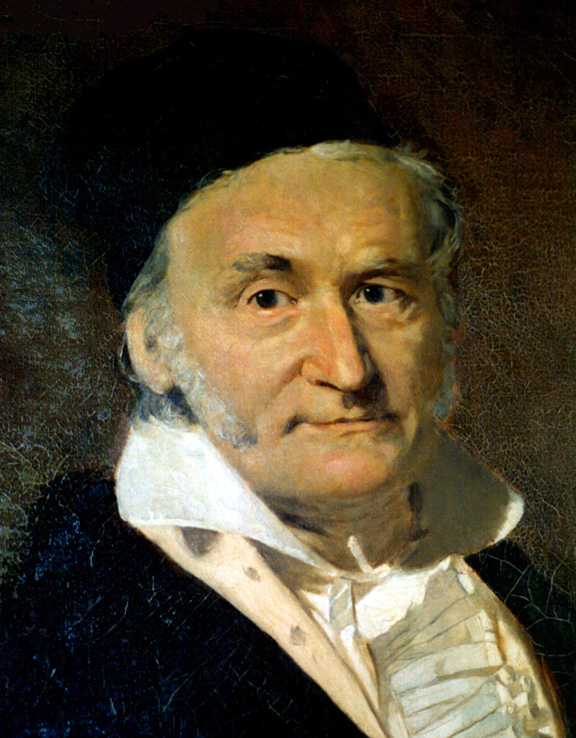
\includegraphics[width=6cm,height=\textheight,keepaspectratio]{Gauss.jpg}

}

\caption{CF Gauss}

\end{figure}%




\end{document}
